\documentclass[a4paper, 11pt]{article}
\setlength{\topmargin}{0.0in}
\setlength{\textheight}{9in}
\setlength{\oddsidemargin}{.2in}
\setlength{\textwidth}{6in}
\usepackage{parskip}
\usepackage{xkeyval}
\usepackage{graphicx}
\graphicspath{ {images/} }
\usepackage{rotating}

\usepackage{tocbibind}
\usepackage[toc,page]{appendix}
\usepackage{datetime}
\usepackage[font={small,it}]{caption}
\usepackage{listings}
\usepackage[font={small,it}]{subcaption}
\usepackage{amssymb,amsmath}
\usepackage{ragged2e}
\renewcommand{\baselinestretch}{1.1}

\newdateformat{monthyeardate}{%
  \monthname[\THEMONTH], \THEYEAR}

\date{}
\begin{document} 

\LARGE\title{Real Time Tempo Analysis of Drum Beats}

\LARGE\author{Author: \textbf{Philip Hannant}, Supervisor: \textbf{Professor Steve Maybank}\\
\\Birkbeck, University of London\\
Department of Computer Science and Information Systems\\
\\Project Report\\
MSc Computer Science\\
\\\monthyeardate\today\\
\vspace{60mm}
}

\normalsize
\maketitle
\section*{}
\begin{justify}
This report is substantially the result of my own work, expressed in my own words, except where explicitly indicated in the text. I give my permission for it to be submitted to the JISC Plagiarism Detection Service. The report may be freely copied and distributed provided the source is explicitly acknowledged.
\end{justify}


\clearpage
\maketitle
\section*{Abstract}
This project report presents an investigation into the suitability of three beat detection algorithms to be used in a drumming training tool. The system captures live audio and passes it to the beat detection algorithms for tempo calculation. The result of which is then passed back to the user.\par

An extensive sample set of drum beats were created to replicate a drummer's performance. The samples were processed through the system and the calculated tempo results recorded. The collected data was then analysed regarding if any of the three beat detection algorithms could be used to form the basis for a future training tool. 

\maketitle
\newpage
\tableofcontents
\clearpage

\section*{Abbreviations}
\begin{tabular}{l p{4.5in}  }\\
\textbf{BPM} & Beats Per Minute\\
\textbf{DFT} & Discrete Fourier Transform\\
\textbf{DWT} & Discrete Wavelet Transform\\
\textbf{JSON} & JavaScript Object Notification\\
\textbf{PW} & Performance Worm\\
\textbf{SBT} & Simple Build Tool\\
\textbf{STFT} & Short Time Fourier Transform\\
\textbf{TDD} & Test Driven Development\\
\end{tabular}

\section*{Definitions}
\begin{tabular}{l p{4.5in}}\\
\textbf{Acoustic Drum Kit} & A collection of drums and cymbals which do not have electronic amplification. Typically made up of a bass drum, snare drum, tom-toms, hi-hat and 1 or more cymbals.\\\\
\textbf{Beat} & For the purpose of this project a beat is defined as the sequence of equally spaced pulses used to calculate the tempo being played by the drummer.\\\\
\textbf{Drum Module} & The device which serves as a central processing unit for an electronic drum kit, responsible for producing the sounds of the drum kit.\\\\
\textbf{Electronic Drum Kit} & An electrical device which is played like an acoustic drum kit, producing sounds from a stored library of instruments and samples.\\\\
\textbf{MIDI} & Musical Instrument Digital Interface is a protocol developed in the 1980's to allow electronic instruments and other digital musical tools to communicate with each other \cite{midi}.\\\\
\textbf{Tempo} & The speed at which a piece of music is played \cite{oxford-comp} and counted in beats per minute (bpm).\\\\
\end{tabular}
\clearpage

\maketitle{} \section{Introduction and Background}

This project report details the aim to develop a real-time drum beat tempo analysis system. The system will use different beat detection algorithms and be able to record the performance of each method when an extensive set of drum samples, representing a real drummer's performance, is processed through the system.

\subsection{Drumming Training Tools Background}
Timing is the fundamental skill any good drummer should possess and is the staple by which they are judged. For many years the only training tool available to a drummer to improve their timing was the metronome, which is an instrument used to mark musical tempo. The metronome was erroneously attributed to Johann Nepomuk Maelzel in 1815 but was invented by a Dutchman, Dietrich Nikolaus Winkel a year earlier. The traditional metronome, based on Winkel's original design is a hand-wound clockwork instrument that uses a pendulum swung on a pivot to generate the ticking, which depicts the desired tempo \cite{brit-metro} and is still used today by musicians, as seen in Figure~\ref{fig: TradMet}. \par

\begin{figure}[ht]
	\centering
	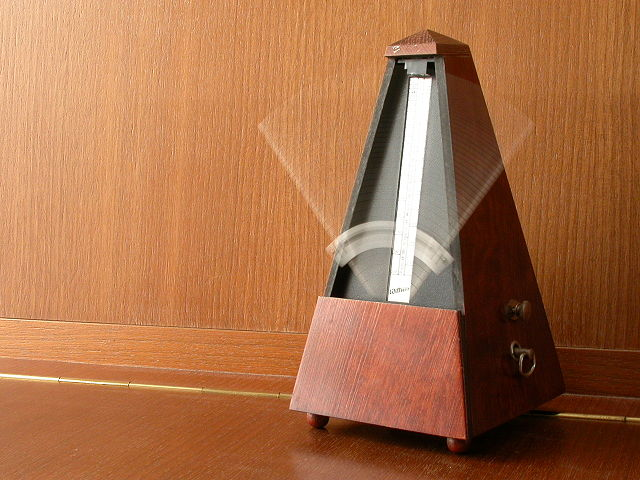
\includegraphics[scale=0.25]{TradMet}
	\caption{Traditional Metronome}% (Source: https://commons.wikimedia.org/w/index.php?curid=1058005)}
	\label{fig: TradMet}
\end{figure}

Today drummers commonly use electronic versions of the metronome are much more widely used, which now developed with functions specifically tailored to a drummers training requirements. The Tama Rhythm Watch (Figure~\ref{fig: RW200}) was the first metronome designed specifically for drummers, providing enough volume to be used with real drums as well as allowing for the use of different time signatures\footnote{A details explanation of time signatures can be found in section~\ref{sec: ts}} and preset rhythm patterns to help improve performance.\par

\begin{figure}[htbp]
	\centering
	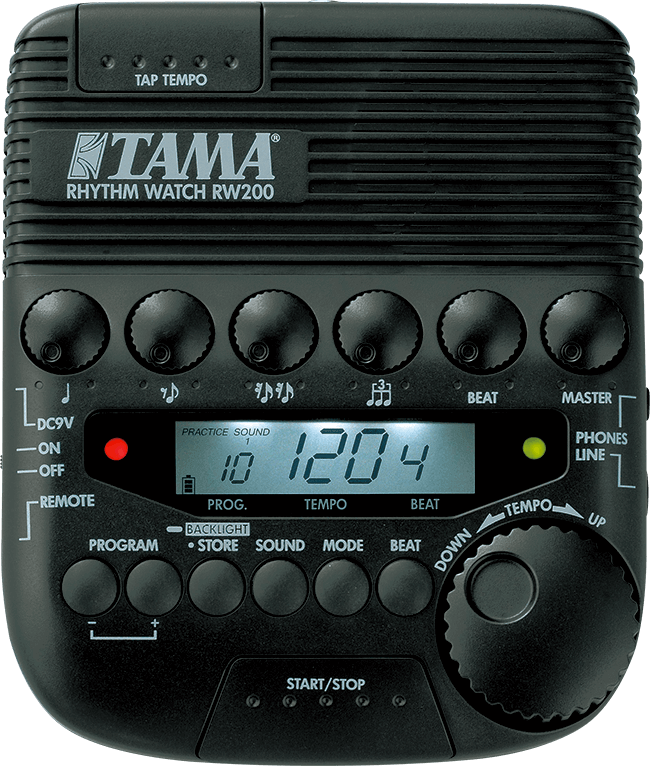
\includegraphics[scale=0.2]{RW200}
	\caption{Tama Rhythm Watch}% (Source: http://www.tama.com/eu/products/accessories/RW200.html)}
	\label{fig: RW200}
\end{figure}

Following the development of the MIDI driven electronic drum kit came the development of more advanced training tools, able to provide live feedback to a drummer during any given performance. Today the leaders in this field are Roland. Their V-Drums line provide a variety of tuition packages including the SCOPE and more recently the COACH system provided in their drum modules. The SCOPE system provides live feedback to a drummer by plotting their performance on a grid representing the elements of the drum kit, Figure~\ref{fig: scope}. The COACH system offers an improved user experience by providing an accuracy figure relating to the number of hits that the drummer has played in time, Figure~\ref{fig: coach}.
\begin{figure}[ht]
\centering
\begin{subfigure}{.5\textwidth}
  \centering
  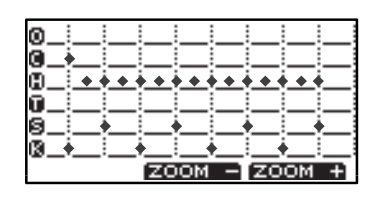
\includegraphics[width=0.5\linewidth]{images/Scope.jpg}
  \caption{Screen shot of the SCOPE system}
  \label{fig: scope}
\end{subfigure}%
\begin{subfigure}{.5\textwidth}
  \centering
  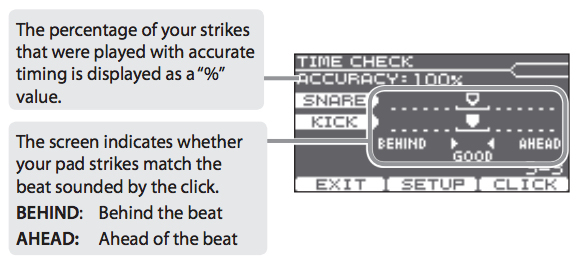
\includegraphics[width=0.75\linewidth]{images/coach.jpg}
  \caption{Screen shot of the COACH system}
  \label{fig: coach}
\end{subfigure}
\caption{SCOPE and COACH training tools}
\label{fig: systems}
\end{figure}

% The V-Drum Rhythm Coach line is an advanced version of the traditional practice pad, which utilises the COACH system (Figure~\ref{fig: rmp-5}. 

The Roland catelogue also includes the DT-1 tutor software package, which provides drummers with an interactive experience helping to improve their rhythm, coordination and sight reading (Figure~\ref{fig: dt-1}).\par 
\begin{figure}[ht]
\centering
% \begin{subfigure}{.5\textwidth}
%   \centering
%   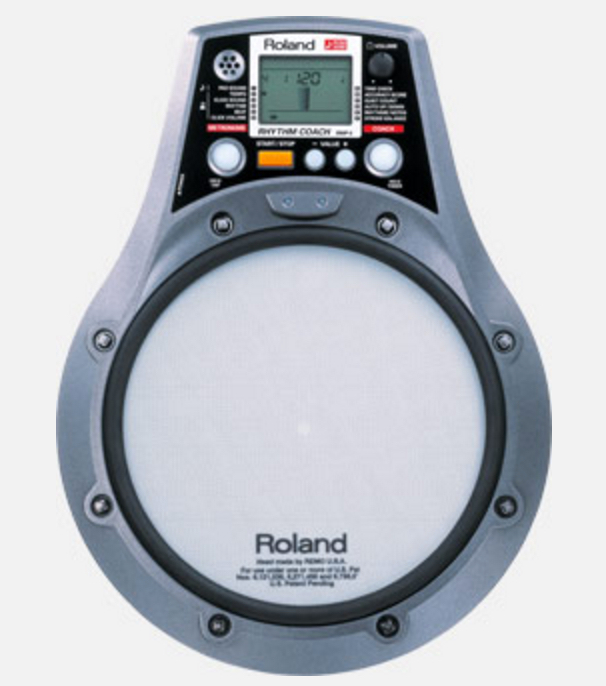
\includegraphics[width=0.5\linewidth]{images/rmp-5.jpg}
%   \caption{The RMP-5 Rhythm coach practice pad}
%   \label{fig: rmp-5}
% \end{subfigure}%
% \begin{subfigure}{.5\textwidth}
  \centering
  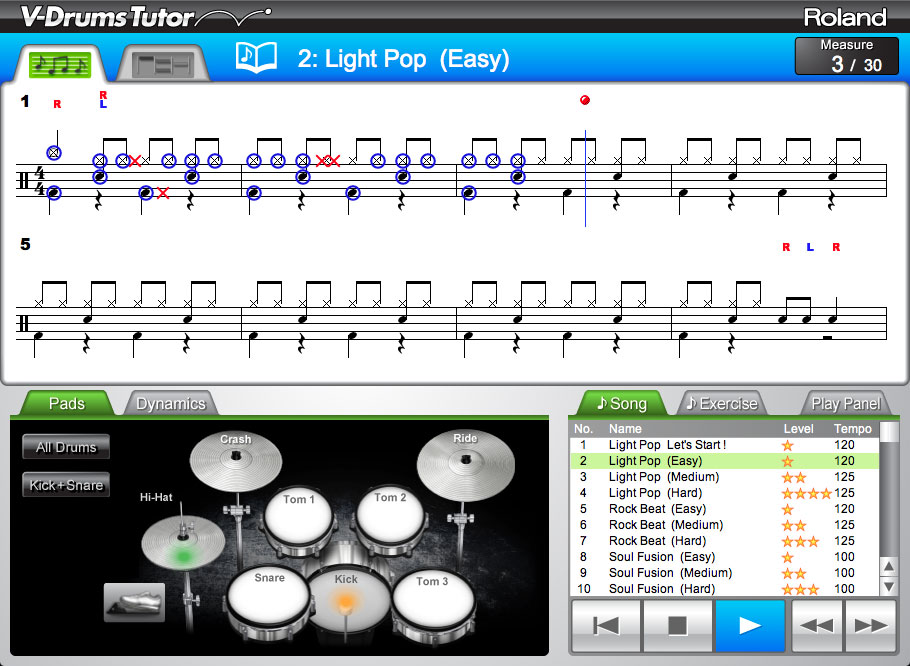
\includegraphics[width=0.5\linewidth]{images/dt-1_ss_main_notation_gal.jpg}
  \caption{Screen shot of the DT-1 V-Drums Tutor}
  \label{fig: dt-1}
% \end{subfigure}
% \caption{}
% \label{fig: roland systems}
\end{figure}
Roland have even started to design games within this field. Their latest release, the V-Drums Friend Jam app, provides the player with live feedback and evaluates each performance to provide the player with a score, which can shared over social media (see Figure~\ref{fig: friendjam}). \par

\begin{figure}[htbp]
\centering
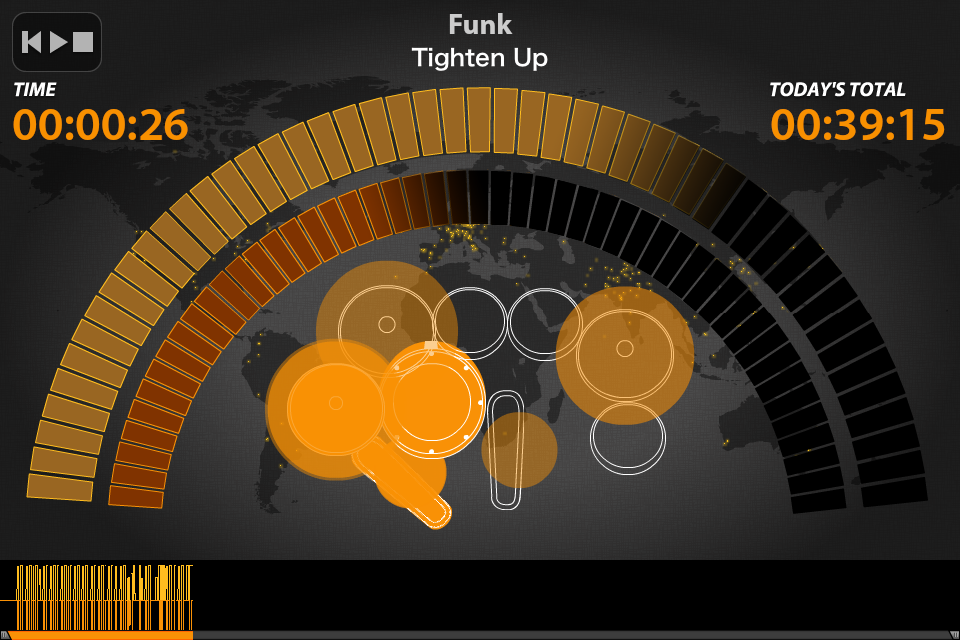
\includegraphics[scale=0.2]{images/friendjam.png}
\caption{Example of the Roland Friend Jam software package}
\label{fig: friendjam}
\end{figure}

Despite these developments there have been a limited number of tools available to be used with acoustic drums. A look at the the App Store\footnote{Apple's application store - itunes.apple.com/uk/appstore‎} and Google Play\footnote{Google's application store for Android devices - play.google.com/store}, reveals a small number of general live bpm detectors but no applications focused towards a drummers training needs.\par

\subsection{Drum Musical Theory}
In order to understand the fundamentals of musical timing some theory needs to be examined. Firstly, the concept of a drummer playing time must be considered. Time, in a drumming sense is an informal term used to describe the consistent rhythmic pattern that a drummer will play on the hi-hat or ride cymbal \cite{drum-bible} and it can be considered one of the most important components of any drum beat. It is also important to note that when a drummer is playing a drum beat, they may play one or more parts of a drum kit simultaneously.  

\subsubsection{Notation}
Drum music notation is written on staff, which is made up of five individual lines (Figure~\ref{fig: staff}). The clef found on the far left of the staff indicates the pitch of the notes \cite{oxford-comp} and as percussion instruments are non-pitched they use the percussion-clef. On traditional musical notation, the lines and spaces between them represent a tone to be played. However, as drums are not considered tonal, the notes written on the staff indicate a certain drum or cymbal. The staff is separated into individual measures which are known as bars \cite{drum-note} and it is these bars that are the basis of musical time. A bar of drum music typically consists of different notes representing which instruments to be played and when. The number of notes within a bar may also vary depending on their length. 

\begin{figure}
	\centering
	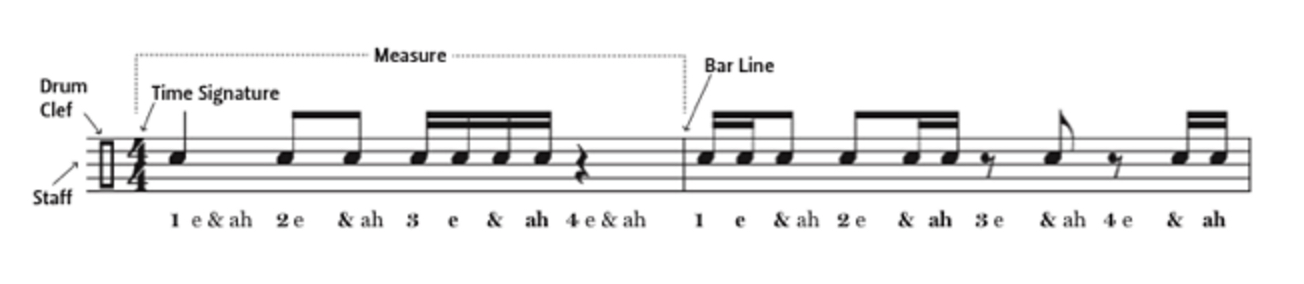
\includegraphics[scale=0.3]{images/staff.jpg}
	\caption{Example of a staff used in musical notation}
	\label{fig: staff}
\end{figure}

\subsubsection{Notes}
The notes used in drum notation not only represent the percussive instrument to be played but also the duration it should be played for. Notes come in different lengths and the key values are the whole (1/1), half (1/2), quarter (1/4), eighth (1/8) and sixteenth (1/16). For example, two eighth notes represent the same time value as a single quarter note. It is also possible to divide note values by three instead of two, these notes are known as triplets. An eighth note triplet is played fifty percent faster than a normal eighth note, therefore for every two eighth notes there are three eighth note triplets \cite{drum-note}. An example of the eighth-note triplets being used is in a twelve eight (12/8) jazz shuffle, the time element played on the ride cymbal or hi-hat is charaterised by playing the first and third triplet of an eighth-note triplet grouping \cite{drum-bible}. Although, such a time element on a cymbal is not considered to be a beat, the notes produced by the action of playing a cymbal need to on the beat. Therefore, for the purpose of this project, it is the count of the prominent beats within a drum beat that are used to calculate a drum beat's tempo.


\subsubsection{Time Signatures}\label{sec: ts}
Time signatures appear on the staff just after the clef and are written as a fraction where the top number indicates the number of beats that there are in a bar, as seen in Figure~\ref{fig: staff}. With the bottom number representing the size of the note that makes up the duration of one beat. For example the straight time four four (4/4) or common time signature indicates four beats in each bar or measure where each beat is made up of one quarter note \cite{drum-note}. Within these bar lines beats can be further divided by using a technique known as subdivision, which is a method for reducing the pulse or rhythm pattern into smaller parts than those originally written. For example, counting a four four (4/4) measure in eighth (1/8) or sixteenth (1/16) notes. 

\subsubsection{Playing Basics}
With the basics of drum theory covered it is now possible to discuss the key elements of a drum beat. Typically for a straight four four (4/4) beat, the bass drum is played on the first and third beat and the snare drum is played on the second and fourth beat both as quarter notes. This is more commonly known as a back beat \cite{drum-bible}. This just leaves the time element which is usually played on the ride cymbal or hi-hat, this too could be played using quarter notes on the first, second, third and forth beats. However, in order to make the drum pattern more dynamic the time element is played using subdivisions, typically using eighth note subdivisions. The ride cymbal or hi-hat will therefore be played on the first, second, third and forth beats as well as the eighth notes in-between each quarter note. This can be demonstrated by counting the one-and-two-and-three-and-four-and, where the ``and'' represents the subdivided eighth note. Playing time on the ``and'' note is also known as playing on the off beat. \par

Additionally to this technique a drummer will usually ensure that there is difference in the volume of the eighth notes being played on the quarter notes and those being played on the ``and''. This technique of emphasising certain beats is known as accenting. 


\subsection{Beat Detection Background}
Most of the early work on beat detection was a by-product of research directed at other areas of musical understanding. Some of the first work in this field can be attributed to H. C. Longuet-Higgins. In 1976, whilst studying the psychological theory of how Western musicians perceive rhythmic and tonal relationships between musical notes, he produced an algorithm capable of following the beat of a performance and adjust the perceived tempo accordingly\cite{allen-danneburg}. Longuet-Higgins' work was built on the premise that in order to perceive the rhythmic structure of a melody it is first necessary to identify the time at which each beat occurs \cite{longeut1}, otherwise know as onset detection. The onset of a note is the instant which marks the start of the variation in the frequency of a signal, a visualisation of this can be seen in Figure~\ref{fig: Onset}. Once detected it can then be used to measure the onset times of sonic events\footnote{A sonic event is a singular feature of a piece music which can be made up of one source or many \cite{sonic}, e.g. the hitting of a drum} within a piece of music \cite{mirex-onset}. These onset times are then used within a beat detection algorithm in order to calculate a piece of music's tempo. 

\begin{figure}[ht]
	\centering
	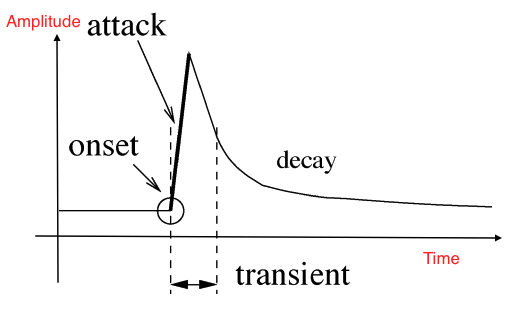
\includegraphics[scale=0.40]{Onset}
	\caption{The onset of a note is the instant which marks start of the variation in the frequency of a signal (Image Source: \cite{onset-tut})}
	\label{fig: Onset}
\end{figure}

Since Longuet-Higgins' first work the area of beat detection has expanded rapidly. In 2005, the first annual Music Information Retrieval Evaluation eXchange (MIREX) was held. MIREX includes a contest with the goal of comparing state-of-the-art algorithms for music information retrieval \cite{mirex-main} and the topics to be evaluated are proposed by the participants. In the first year, three of the nine topics concerned beat detection, including audio onset detection and since it's first inclusion it has been an evaluated topic of all but one of the last twelve contests \cite{mirex-onset}. The beat detection algorithms proposed to perform the tempo analysis for this project, the Beatroot system developed by Simon Dixon \cite{dixon1} and a development on the original audio analysis using the Discrete Wavelet Transform (DWT) by Tzanetakis, Essel and Cook \cite{tzane1}. Are both former entrants to the MIREX contest, with the Beatroot system receiving the highest score in the 2006 Audio Beat Tracking task \cite{mirex-06} 

\subsection{Project Aims}
The primary aim of this project is to investigation whether some of the currently available beat detection algorithms are accurate enough to be used in a training tool for drummers practicing on an acoustic drum kit. In order to achieve this the developed software package, hereafter referred to as  RTT\_Analyser\footnote{Where RTT stands for Real Time Tempo}, will need to process enough live audio in form of sampled drum beats and record each of the chosen beat detection algorithms accuracy. 

The original core features of the RTT\_Analyser developed for this project are:

\begin{enumerate}
\item A live audio tempo analysis tool, that compares and records the performance of selected beat detection algorithms
\item The RTT\_Analyser implements an adapted version of the beat tracking system Beatroot and the DWT algorithm described by Tzanetakis \textit{et al} \cite{tzane1}.
\item RTT\_Analyser implements a system capable of parallel processing, allowing for the same captured live audio data to be sent to the chosen beat detection algorithms in order for the tempo to be calculated simultaneously.
\item While processing live audio the RTT\_Analyser stores a predetermined data set in order to allow for performance analysis of the beat detection algorithms.
\item The RTT\_Analyser will provide the user with real time feedback of the most recent tempo calculation returned
\item An extensive sample set of drum beats will need to be created. The samples will be produced with exact tempos in order to provide a ground truth regarding the accuracy of the beat detection algorithms. 
\end{enumerate}



\maketitle{}\section{RTT\_Analyser Beat Detection Algorithms}
The original proposed solution incorporated two beat detection algorithms, the Beatroot system \cite{dixon1} and the DWT method \cite{tzane1}. However, the adaptation of the Beatroot system to be used with live audio took longer than the proposed time-frame. This meant that an alternative system needed to be found in order to mitigate this issue, conveniently the Beatroot software package also contained another beat detection system, the Performance Worm \cite{dixon3}. To ensure the project remained on track it was decided to substitute the Performance Worm for the Beatroot system. With the intention, once the project was back on schedule, to resume the adaptation of the Beatroot system to work with live audio. This was successfully completed prior to the development of the user interface.

The project report will now discuss the three beat detection algorithms incorporated in the RTT\_Analyser.

\subsection{Beatroot}
Beatroot is a beat detection software package created by Simon Dixon \cite{dixon1}, designed to extract musical expression information from musical recordings \cite{dixon3}. The algorithm designed by Simon Dixon is ideal for the RTT\_Analyser as it is considered sufficiently fast enough to be implemented as part of a real-time system \cite{dixon4}.\par

Beatroot is comprised of two major components, the tempo induction and the beat tracking subsystems. Before tempo induction can take place, first a list of onsets needs to be retrieved\cite{dixon4}. This is achieved by obtaining a time-frequency representation with a Short Time Fourier Transform (STFT). The STFT is based on the Discrete Fourier Transform (DFT), which can be used to determine how much of a frequency exists within a signal. However, the DFT is unable to provide any details of when a frequency component occurs in time for non-stationary signals\footnote{Non-stationary signals are signals whose frequency contents changes over time \cite{polikapt2}}. A solution to this is to split a non-stationary signal into a number of smaller segments using a window function, which effectively creates a series of stationary\footnote{The frequency contents of a stationary signal does not change over time} signals which the DFT can then be applied to. By splitting the signal into smaller segments the STFT is able to apply the DFT to these segments and essentially express a signal as a linear combination of elementary signals that are easily manipulated. The DFT returns a spectrum containing information about how the energy held within the signal is distributed in the time and frequency domains \cite{tzane2}.\par

The window function used by Beatroot within the STFT is known as a Hamming window, which can help to reduce the amount of additional frequencies appearing in the returned DFT spectrum, known as spectral leakage. This is caused when the steep slope of a rectangular window (Figure~\ref{fig: rectan}) causes the frequencies to become distorted. The Hamming window counteracts this by using a bell shape, which reduces the amplitudes of its sidelobes \cite{lyons} and ensures the spectrum returned is less spread out and closer to the ideal theoretical result \cite{tzane2}. A visualisation of a Hamming window can be seen in Figure~\ref{fig: hamWin}. 

\begin{figure}[ht]
\centering
\begin{subfigure}{.5\textwidth}
  \centering
  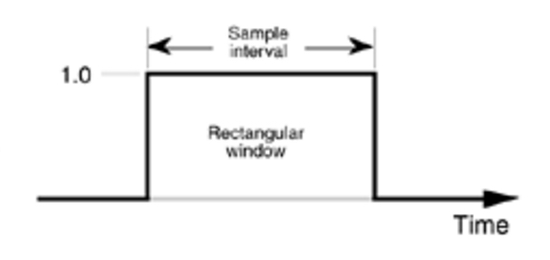
\includegraphics[width=0.6\linewidth]{images/rectangWin.jpg}
  \caption{Rectangular window}
  \label{fig: rectan}
\end{subfigure}%
\begin{subfigure}{.5\textwidth}
  \centering
  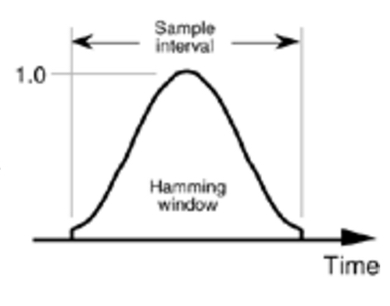
\includegraphics[width=0.6\linewidth]{images/hamming.jpg}
  \caption{Hamming window}
  \label{fig: hamWin}
\end{subfigure}
\caption{(Image Source: \cite{lyons})}
\label{fig: Wins}
\end{figure}

The STFT used by Beatroot is defined as follows:
\begin{equation}
\begin{split}
X(n, k) = \sum_{m=-\frac{N}{2}}^{\frac{N}{2}-1} x(hn+m)\hspace{2mm}w(m)\hspace{2mm}e^-{\frac{2jπmk}{N}}
\end{split}
\end{equation}
Where a Hamming window $w(m)$ is calculated at a frame rate of 100 Hz, $N$ is the size of the window, and $n$ represents the frame number being processed. The index of frequency-domain component is represented by $k$, and $h$ is the hop-size or number of samples between the start times of adjacent frames.

The spectral flux function is then used as a method for measuring the change in magnitude of each returned frequency-domain sample \cite{dixon2} and is provided by: 

\begin{equation}
\begin{split}
SF(n) = \sum_{k=-\frac{N}{2}}^{\frac{N}{2}-1} H(|X(n,k)| - |X(n-1, k)|)
\end{split}
\end{equation}

Where $SF$ is the spectral flux and $H$ is the half-wave rectifier function given by the $H=\frac{x+|x|}{2}$, which is used to remove any negative values representing a falling signal. An example of the peaks returned by a spectral flux function can be seen in Figure~\ref{fig: spec-flux}.

\begin{figure}[ht]
	\centering
	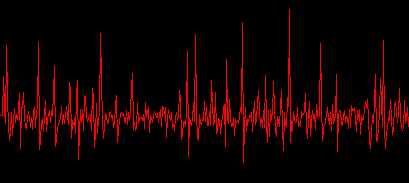
\includegraphics[scale=0.5]{images/spectralflux.png}
	\caption{(Image Source: \cite{badlogic})}
	\label{fig: spec-flux}
\end{figure}

The onsets detected are then selected by a peak-picking algorithm which finds local maxima within the detection function. The tempo induction algorithm is then used to compute clusters of inter-onset intervals (IOI) by using the calculated onset times. Each cluster represents a hypothetical tempo, in seconds per beat \cite{dixon1}. The clustering algorithm works by assigning an IOI to a cluster if its difference from the cluster is less than 25ms. The cluster information is then combined by recognising the approximate integer relationships between clusters. An example of this can be seen in Figure~\ref{fig: br-clusters} where cluster C2 is twice as long as C1 and C4 is twice that of C2. This information along with the number of IOIs within a cluster is then used to weight each cluster which is then returned as a ranked list of tempo hypotheses \cite{dixon4}.

\begin{figure}[ht]
	\centering
	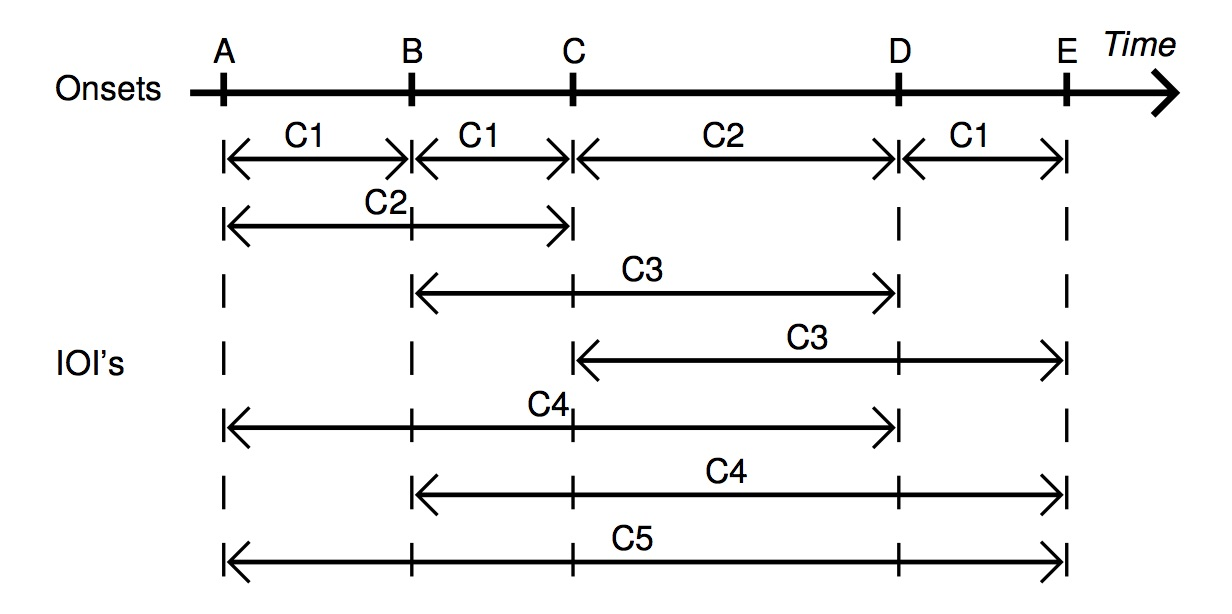
\includegraphics[scale=0.25]{br-clusters}
	\caption{(Image Source: \cite{dixon4})}
	\label{fig: br-clusters}
\end{figure}

The multiple agent architecture of Beatroot's beat tracking subsystem is then employed to find the sequences of events that closest match the original tempo hypotheses, these sequences are rated and the most likely set of beat times is determined. Each of the agents are initialised with a tempo or beat rate hypothesis and an onset time. Further beats are then predicted by the agent based on these parameters. Any onsets corresponding with the predicted beat times are taken as a beat time, those falling outside are not considered to be a beat time. The agents then rate themselves based on how evenly spaced the beat times are, the number of predicted beats which relate to actual events, and the salience\footnote{The salience is a measure of the note duration, density, pitch and density \cite{dixon1}, which is calculated from the spectral flux of the onset \cite{dixon4}} of the matched onsets. The agent with the highest score is then returned as the sequence of beats corresponding to the processed audio \cite{dixon4}, which is then used to determine the overall tempo of the audio by using the ``inter-beat intervals, measured in beats per second'' \cite{dixon1} to calculate beats per minute (bpm) of the audio.


\subsection{Discrete Wavelet Transform and Beat Detection Method}
The wavelet transform is a technique for analysing signals which was developed as an alternative to the STFT \cite{tzane1}. Like the STFT, the DWT is able to provide time and frequency information, however, unlike the STFT the DWT is able to do this without the need for a window function. Instead, the DWT uses a variable time-frequency resolution that allows for low frequencies to be detected precisely but not accurately placed in the time, and high frequencies to be accurately placed in time but not detected as precisely. The most common type of DWT can be viewed as a filter-bank, where each of the filters corresponds to a certain frequency range, usually representing an octave in frequency\footnote{Acoustically, an octave above a note is the note which has twice the frequency of the original \cite{oxford-comp}.}\cite{tzane2}.

In 2001, Tzanetakis \textit{et al} described how the DWT could be used to extract information from non-speech audio \cite{tzane1}. Their beat detection algorithm was based on detecting the most prominent signals which are repeated over a period of time within the analysed audio. \par

The first stage is to split the signal into a number of octave frequency bands using the DWT. This allows for the time domain amplitude envelopes of each frequency band to be extracted separately, using the following three steps. Where $x[n]$ is the input signal and $y[n]$ the output: 


\begin{enumerate}
\item Full Wave Rectification:
\begin{equation}
\begin{split}
y[n] = |x[n]|
\end{split}
\end{equation}
a process of converting the amplitude of each frequency band to one polarity \cite{pallas}, which can be either positive or negative. Performed in order to extract only the time-related envelope of the signal as opposed to the time domain signal itself \cite{tzane3}. 
\item Low Pass Filtering:
\begin{equation}
\begin{split}
y[n] = (1 - \alpha)x[n] + \alpha y[n - 1] 
\end{split}
\end{equation}
for a single frequency point where $\alpha$ has a value of 0.99. Designed to allow frequencies below a cutoff frequency through but blocks any frequencies above the cutoff frequency \cite{smith}. Used in this context as a way to smooth the signal within envelope \cite{tzane3}.
\item Down-sampling:
\begin{equation}
\begin{split}
y[n] = x[kn]
\end{split}
\end{equation}
where $k$ was set to a value of 16. Due to the large periodicities in beat analysis, the signal is down-sampled in order to reduce the computation time of the autocorrelation stage without causing any negative effects on the performance of the algorithm \cite{tzane3}.
\end{enumerate}

Each frequency band is then normalised through a method of mean removal:
\begin{equation}
\begin{split}
y[n] = x[n] - E[x[n]]
\end{split}
\end{equation}
where $E$ represents the expected mean value. Mean removal is applied to ensure the signal is centred at zero for the autocorrelation stage \cite{tzane3}. The autocorrelation function is then applied to each frequency band:
\begin{equation}
\begin{split}
y[n] = \frac{1}{N}\sum_{n} x[n]x[-k]
\end{split}
\end{equation}
where $N$ represents the sample size. The resulting peaks produced by the autocorrelation function correspond to the various periodicities of that signal's envelope. The first five peaks of the function and their corresponding periodicities are then calculated in beats per minute and added to a histogram. This process is repeated while iterating over the signal. The estimated tempo of the audio signal is then retrieved from the periodicity that corresponds to the highest peak within the histogram \cite{tzane1}. The DWT beat histogram flow diagram can be seen in Figure~\ref{fig: dwtFlow}.

\begin{figure}[ht]
	\centering
	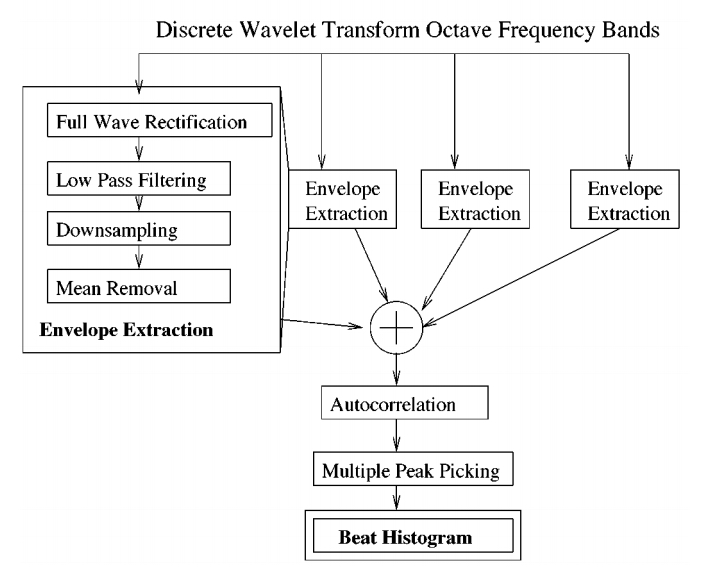
\includegraphics[scale=0.35]{images/dwtflow.jpg}
	\caption{Flow diagram of the beat histogram method described by Tzanetakis \textit{et al} \cite{tzane3}}
	\label{fig: dwtFlow}
\end{figure}


\subsection{Performance Worm}
The final beat detection algorithm employed in the RTT\_Analyser is the Performance Worm (PW) system, designed by Simon Dixon, Werner Goebl and Gerhard Widmer \cite{dixonGoeblWidmer}. The PW is based on a real time algorithm which is able to determine the tempo of input raw audio, while keeping track of other possible tempo hypotheses that are rated and updated dynamically. This allows for the most recently highest ranked tempo hypothesis to be returned to the user \cite{dixonGoeblWidmer}. 

First the PW processes the raw audio which can either be extracted from a static recording or directly from a live input with a smoothing filter\footnote{Process which attempts to reduce any noise found within a signal. A smoothing filter does this by reducing any points in the signal that are higher than adjacent points and reducing those points that are lower than adjacent point \cite{pragmaticSig}} in order to obtain the RMS amplitude\footnote{RMS stands for root mean square and is the process of squaring all of the amplitude values, then taking the average (mean) of the squared values, and then calculating the square root of the average value \cite{rms}.} of the signal taken from a 40ms window. The note onsets are then calculated by the event detection module that finds the slope of the smoothed amplitude and then calculates the set of local peaks which are taken as the note onset times \cite{dixonGoeblWidmer}. 

The signal is then processed by the multiple tempo tracking subsystem which uses a similar approach to the Beatroot system. A clustering algorithm (Figure~\ref{fig: clusterAl}), first calculates the time intervals (inter-onset intervals or IOIs) between the pairs of onsets, which it holds in memory (approximately five seconds of audio). The intervals are then weighted by the mean of the amplitudes and each interval's IOIs are clustered using the best-first algorithm (shown in Figure~\ref{fig: clusterAl}). The significant clusters of IOIs determined by the best-first algorithm are subsequently assumed to be the musical units held within the signal. 

As in the Beatroot system, these clusters are then used as the bases of the tempo hypotheses produced by the tempo tracking subsystem. The tempo inducer then exploits a property of most Western music where time intervals are related by small approximate integer ratios. As the times held by the clusters can be considered to represent related notes, e.g. quarter and eighth notes. The tempo inducer then adjusts cluster times and weightings according to the information held by the sets of related clusters. Two clusters are considered to be related if the ratio of their time intervals is close to an integer. The highest weighted clusters and their respective tempo hypothesis are then returned as the tempo output \cite{dixonGoeblWidmer}.


\begin{figure}
	\hspace{10mm} \textbf{Inter-onset interval calculation}\\
	\hspace*{10mm} For each new onset\\
	\hspace*{20mm} For IOI times $\mathit{t}$ from 100ms to 2500ms in 10ms steps\\
	\hspace*{30mm} Find pairs of onsets which are $\mathit{t}$ apart\\
	\hspace*{30mm} Sum the mean amplitude of these onset pairs\\
	\hspace*{20mm} \\
	\hspace*{20mm} \textbf{Best-first algorithm}\\
	\hspace*{20mm} Loop until all IOI time points are used\\
	\hspace*{30mm} For times $\mathit{t}$ from 100ms to 2500ms in 10ms steps\\
	\hspace*{40mm} Calculate window size $\mathit{s}$ as function of $\mathit{t}$\\
	\hspace*{40mm} Find average amplitude of IOIs in window $\mathit{[t, t + s]}$\\
	\hspace*{40mm} Store $\mathit{t}$ which gives maximum average amplitude\\
	\hspace*{30mm} Create a cluster containing the stored maximum window\\
	\hspace*{30mm} Mark the IOIs in the cluster as used\\
	\hspace*{20mm} \\
	\hspace*{20mm} \textbf{Cluster Combining}\\
	\hspace*{20mm} For each cluster\\
	\hspace*{30mm} Find related clusters (multiples or divisors)\\
	\hspace*{30mm} Combine related clusters using weighted average\\
	\hspace*{20mm} Match combined clusters to tempo hypotheses and update\\
	\caption{Clustering algorithm used in the Performance Worm Multiple Tempo Tracking Subsystem \cite{dixonGoeblWidmer}}
	\label{fig: clusterAl}
\end{figure}

\maketitle{} \section{Solution Design and Architecture}
The basic premise for the RTT\_Analyser is to enable the user to play a live drum beat through the system, the tempo of the live audio is then returned to user while being stored for future analysis. Initially, the RTT\_Analyser opens the inbuilt microphone of the device upon which the software is being run. After establishing the live audio stream the RTT\_Analyser beat detection algorithms are sent the live audio data in the format of a byte array. These live audio bytes are then decoded according to the individual algorithm's requirements before being processed and the tempo calculated.

\subsection{Live Audio Processing}
\label{sec: liveaudio}
The live audio is processed using the Java Sound API, which contains two key types; mixers and lines. Mixers are a representation of the audio devices available on a certain system and a line is an element of the digital audio pipeline responsible for moving audio in and out of the system. Typically, audio capture is started or stopped using a \texttt{TargetDataLine} that provides a path to the systems audio input device. Access to this device is provided by the \texttt{AudioSystem} class, which acts a clearing house for audio components. In order to ensure the bytes of audio data passed through the \texttt{TargetDataLine} are interpreted correctly the \texttt{AudioFormat} object enables the audio format to be defined by the list attributes below \cite{javasound}, which includes the values chosen to ensure that the audio capture by the RTT\_Analyser is comparable to CD quality:

\begin{itemize}
\item Encoding - Set to ``PCM.signed'', representing audio encoded to the native linear pulse code modulation, where pulse code modulation is the process of sampling and quantising the signal into discrete symbols for transmissions \cite{pulseWag}.
\item Sample Rate - 44,100, set to match CD quality for the number of analog samples analysed per second. 
\item Sample Size in Bits - 24, based on a sound card with a 24 bit sample depth.
\item Channels - 2, audio is captured using the built in microphone, typically stereo of the device the RTT\_Analyser is being run on.
\item Frame Size - 6, where the frame size is the number of bytes in a sample multiplied by the number of channels \cite{audioFormat}.
\item Frame Rate - 44,100, same as the sample rate.
\item Big Endian (boolean) - false, as the machine used to develop the RTT\_Analyser has Intel cores, which use a little-endian architecture\footnote{Endianess refers to the order of bytes which make up a digital word. Big endianess stores the most significant byte at a certain memory address and the remaining bytes being stored in the following higher memory addresses. The little-endian formate reverses the order storing the least significant at the lowest and most significant at the highest memory address \cite{endiness}.}.
\end{itemize}

In order to process the captured bytes the RTT\_Analyser required a concurrent system capable of running the three beat detection algorithms in parallel. This was provided by the Akka Actors system.

\subsection{Akka Actors}
The Akka Actor Model is specifically designed to provide the ability to write concurrent systems with a high level of abstraction that removes the need for the developer to handle locking and individual thread management. Making it much easier to write concurrent and parallel systems than with the traditional approaches used in Java \cite{akkaActors}.

A fundamental construct of the Akka Actor system is that it strictly adheres too the Reactive Manifesto, which aims to ensure applications built under this are easier to develop and are amenable to change. This allows for a higher level of tolerance to failure and the ability to meet any such failure elegantly \cite{reactMan}. The Reactive Manifesto requires applications to satisfy one or more of the requirements listed below \cite{reactMan} and visualisation of how they interact can be seen in Figure~\ref{fig: reacMan}.


\textbf{Responsive} - The system responds in a timely manner, if possible. By providing usability and utility responsiveness, it is possible to detect and resolve problems effectively.\\\\
\textbf{Resilient} - The system should be able to remain responsive even in the event of a failure, which applies to all parts of the system not just the mission critical components. To achieve this each component needs to be isolated within the system, therefore allowing failed parts of the system to recover without effecting the responsiveness of the system as a whole.\\\\
\textbf{Elastic} - The system will be able to maintain the same level of responsiveness despite varying workloads. Reacting to changes in the rate of input by adapting the levels of resources allocated accordingly.\\\\
\textbf{Message Driven} - Reactive systems rely on the use of asynchronous message passing in order to establish boundaries between components within the system, ensuring isolation, loose coupling\footnote{Loose coupling is a design approach of distributed systems which emphasises agility and ability to adapt to changes \cite{looseCouple}} and location transparency\footnote{The decoupling of the runtime instances from their references \cite{reactMan}}. By utilising non-blocking\footnote{In concurrent programming algorithms which do not have their execution indefinitely postponed when competing for a resource is said to be non-blocking \cite{reactMan}.} message-passing it is possible to ensure message recipients only consume resources when active, leading to a much reduced system overhead.\\\\

\begin{figure}[ht]
	\centering
	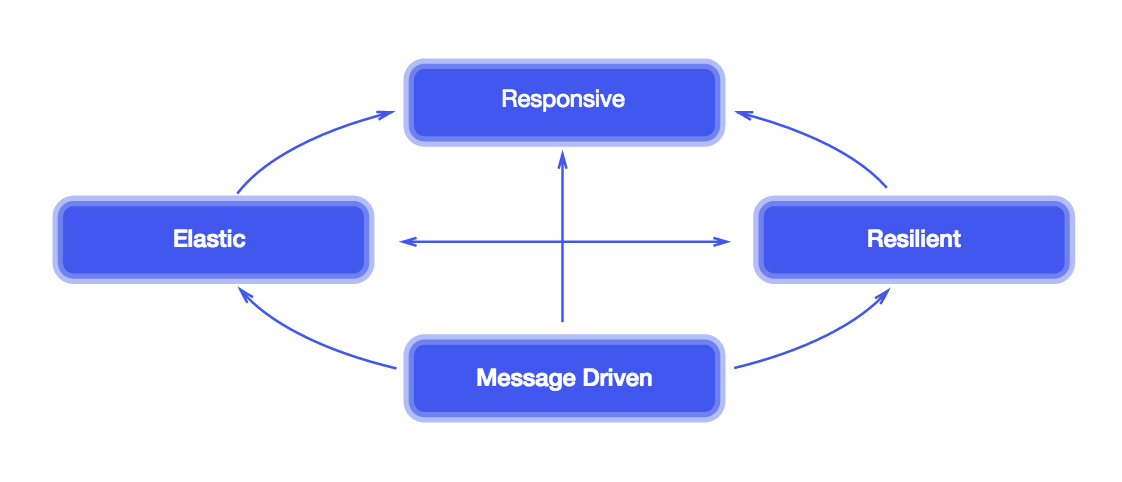
\includegraphics[scale=0.25]{images/reacManif.jpg}
	\caption{Visualisation of the requirements of the Reactive Manifesto interact \cite{reactMan}}
	\label{fig: reacMan}
\end{figure}


\subsubsection{The Actors}
The actors within the actor model are objects that are used to encapsulate state and behaviour. They communicate exclusively through messages passed to a recipients mailbox and it can help to think of them as group of people being assigned subtasks within an organisational structure. One of the key features of an actor system is that tasks are split up and delegated until they become small enough to be handled in one piece. This process ensures that the tasks being carried out by the actors are clearly defined. It also allows for the actors to be designed in terms of the messages they are able to receive and how they should react to these messages and any failures that might occur. The actors within a system will naturally form a set hierarchy. For example, an actor assigned the task of overseeing a certain function might split this function into a number of smaller tasks. It will then assign these tasks to some child actors, which it will supervises until the task is complete \cite{acotrsys}.\par 

The actors created within the RTT\_Analyser were a mix of stand alone actors and actors which were required to supervise subtasks carried out by child actors.

\subsection{Design Pattern}
The RTT\_Analyser was developed using the Model View Controller (MVC) design pattern, as the MVC pattern is the tried-and-tested approach when designing applications with a graphical user interface \cite{designPatterns}. The MVC pattern is made up of the following components and a visualisation of the MVC can be seen in Figure~\ref{fig: mvc}. 

\begin{itemize}
\item \textbf{Model} - is represented by the data and associated applications \cite{designPatterns}, within the RTT\_Analyser the model is provided by the beat detection algorithms, the live audio capturing and processing components.\\
\item \textbf{View} - is the graphical interface displayed to the user which updates itself automatically \cite{designPatterns}. For the RTT\_Analyser the view is represented by the user interface\\
\item \textbf{Controller} - is the part of the application that responds to the user interactions, liasing with both the model and the view components\cite{designPatterns}. The controller for the RTT\_Analyser is the actor system, which is responsible for message passing between the model and view components.
\end{itemize}

\begin{figure}[ht]
	\centering
	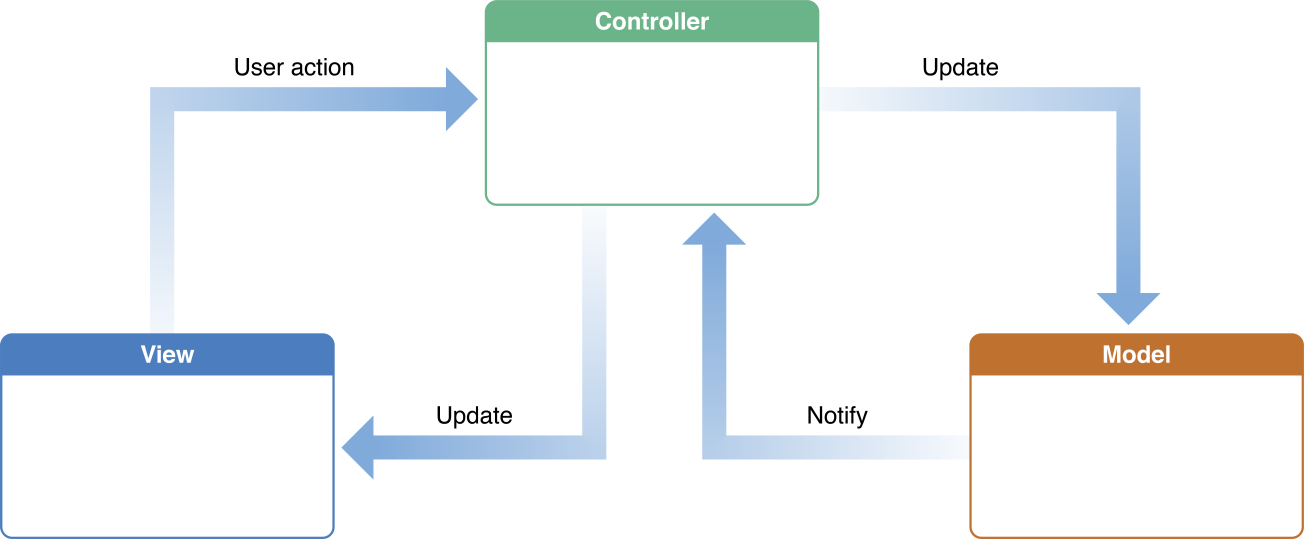
\includegraphics[scale=0.25]{images/mvc.png}
	\caption{The three components which make up Model View Controller design pattern \cite{applemvc}}
	\label{fig: mvc}
\end{figure}

A high level class diagram of the final version of RTT\_Analyser can be seen in Figure~\ref{fig: uml} 

\begin{sidewaysfigure}[htbp]
	\centering
	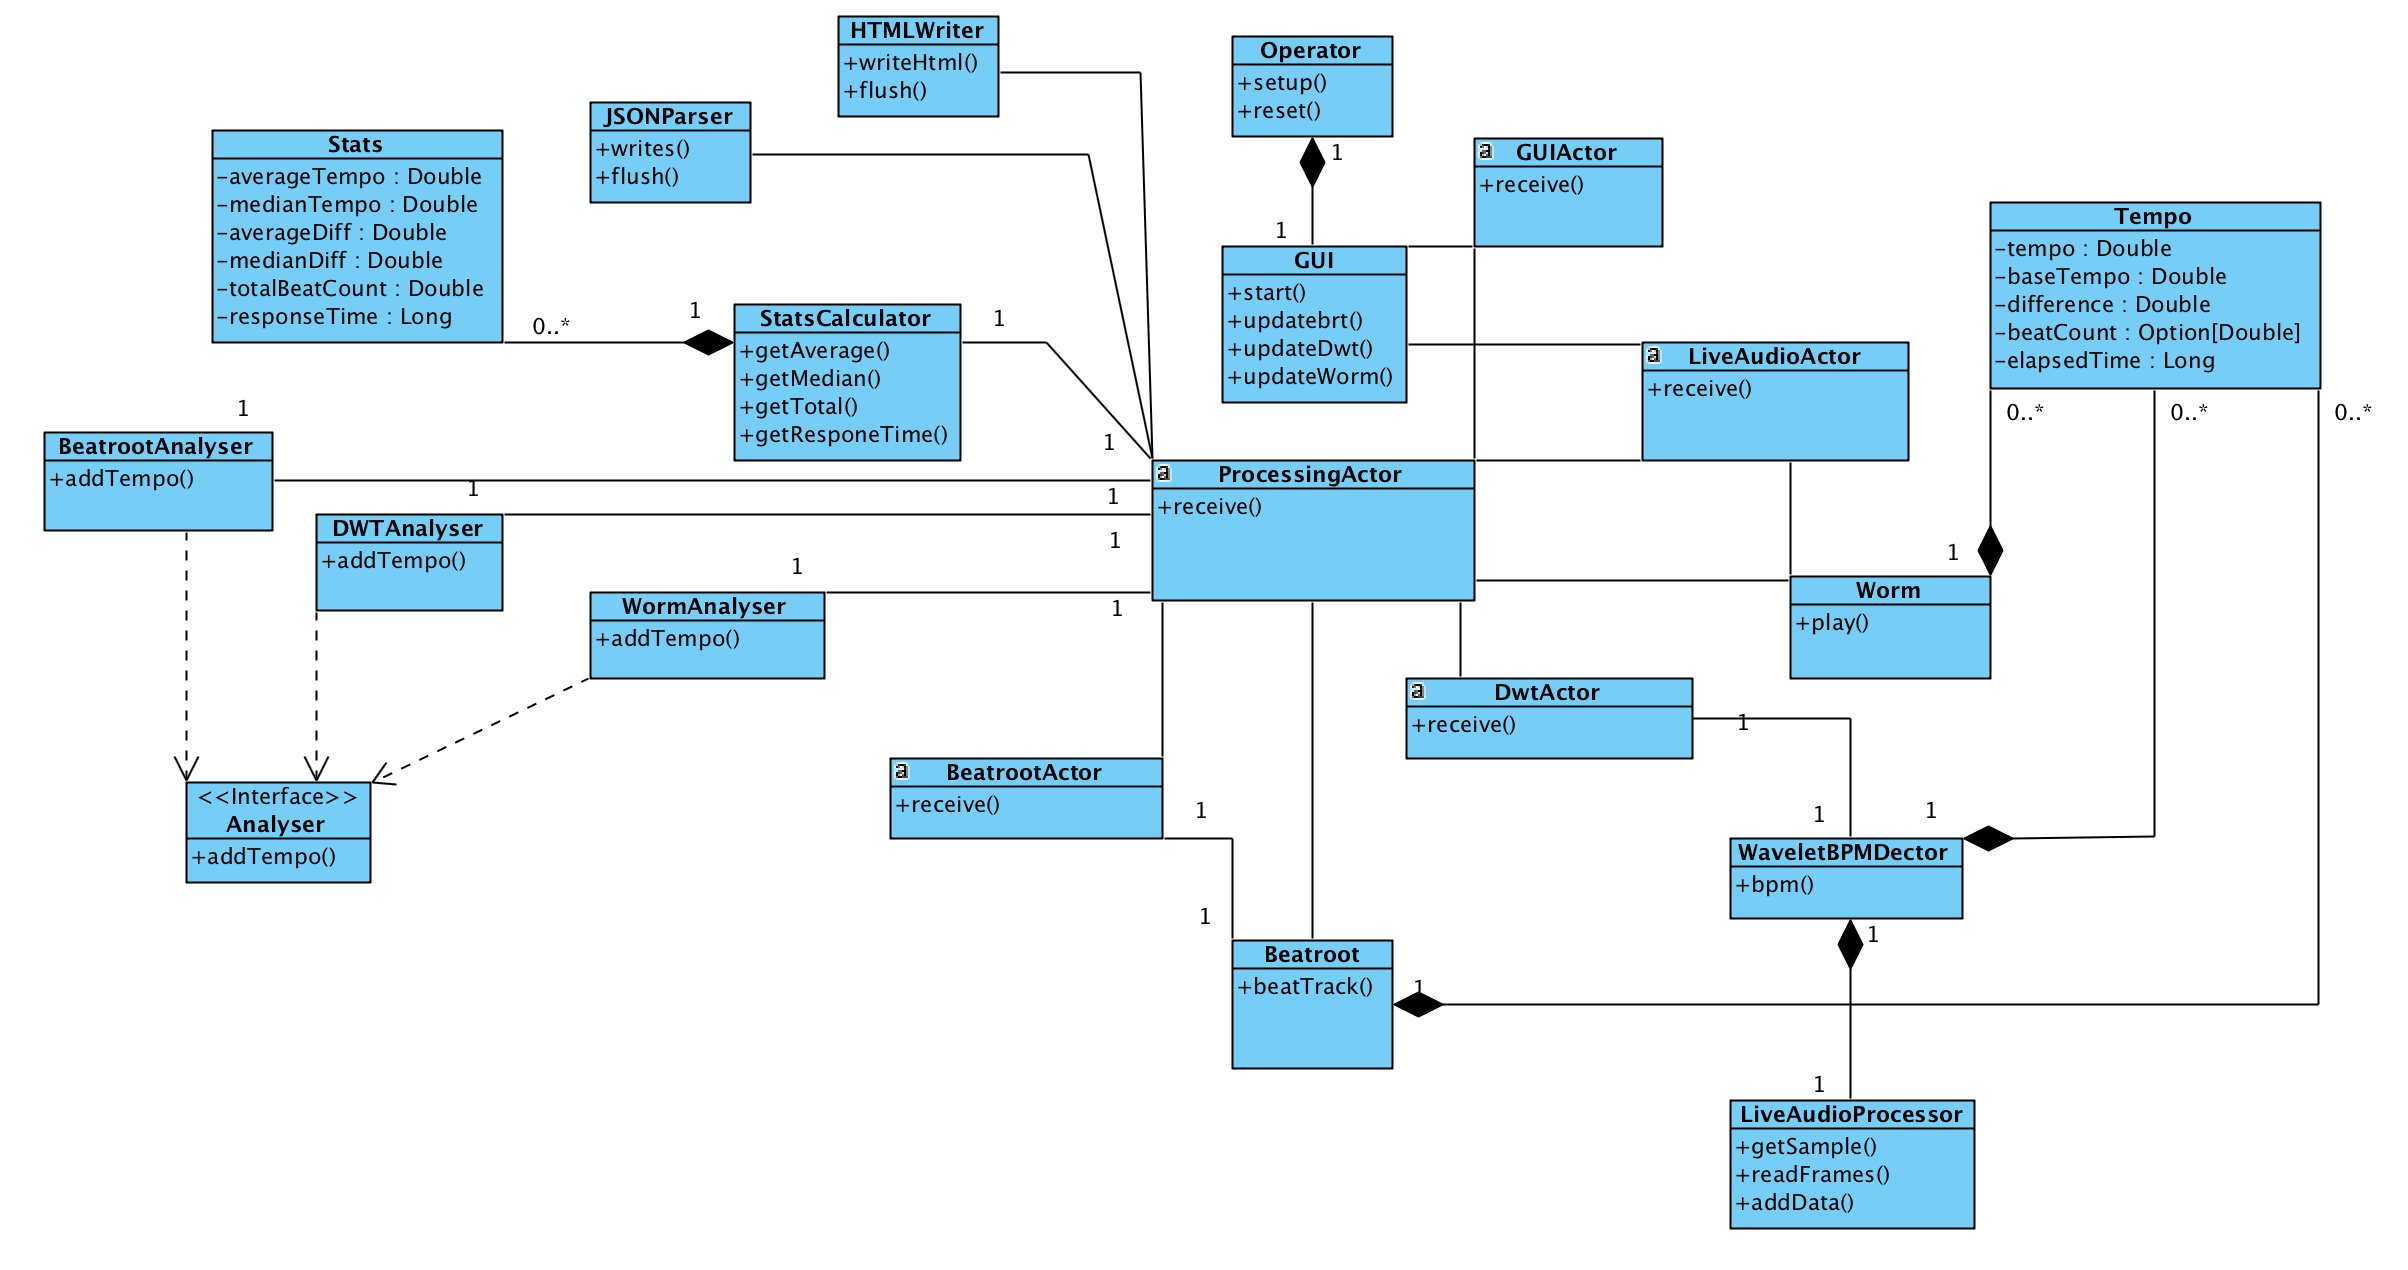
\includegraphics[scale=0.3]{images/RTTUMLDiagram.jpg}
	\caption{Image to be added}
	\label{fig: uml}
\end{sidewaysfigure}


\maketitle{} \section{Implementation}
The RTT\_Analyser is written in Java and Scala, due to the Beatroot and Performance Worm both being written in Java, and the author's familiarity with both languages. Using Scala also ensured the twin constructs of pattern matching and case classes were able to be utilised where appropriate. Pattern matching is used to implement type switches and is considered to create ``code that is both succinct and obviously correct'' \cite{mariusEr}. Case classes are Scala's way of allowing pattern matching to be performed on objects without the need for additional boilerplate code. Using Scala, also allows for more elegant and concise tail recursive\footnote{A recursive solution is considered to be tail recursive if the last operation carried out is to calculate the return value, it has the advantage over recursive calls of not building a stack trace and instead performing each operation in a single stack frame \cite{odesky}} solutions to be developed over loop-based solutions. As the Scala compiler provides an optimiser which ensures that there are not any runtime overheads to be paid for employing tail recursion \cite{odesky}.

The RTT\_Analyser was developed in the Scala specific build tool, sbt (simple build too). The sbt is a build tool that creates a stable build platform that supports a reactive development environment able to re-run all tests when source code is updated \cite{sbt}. In terms of this project sbt was chosen primarily for it's support of mixed Scala/Java projects. Allowing for the Java Beatroot and Performance Worm systems to be easily incorporated with the Scala implementation of the DWT beat detection algorithm and the Akka Actor system.

\subsection{The Actor System}
Although the actors were not the first element of the RTT\_Analysert to be implemented, introducing them first helps to provide some context for the how the other components communicate.\par

The actor system is constructed of five different actors and a diagram of the actor hierachy can be seen in Figure~\ref{fig: actorHe}. 

\begin{figure}[htbp]
\centering
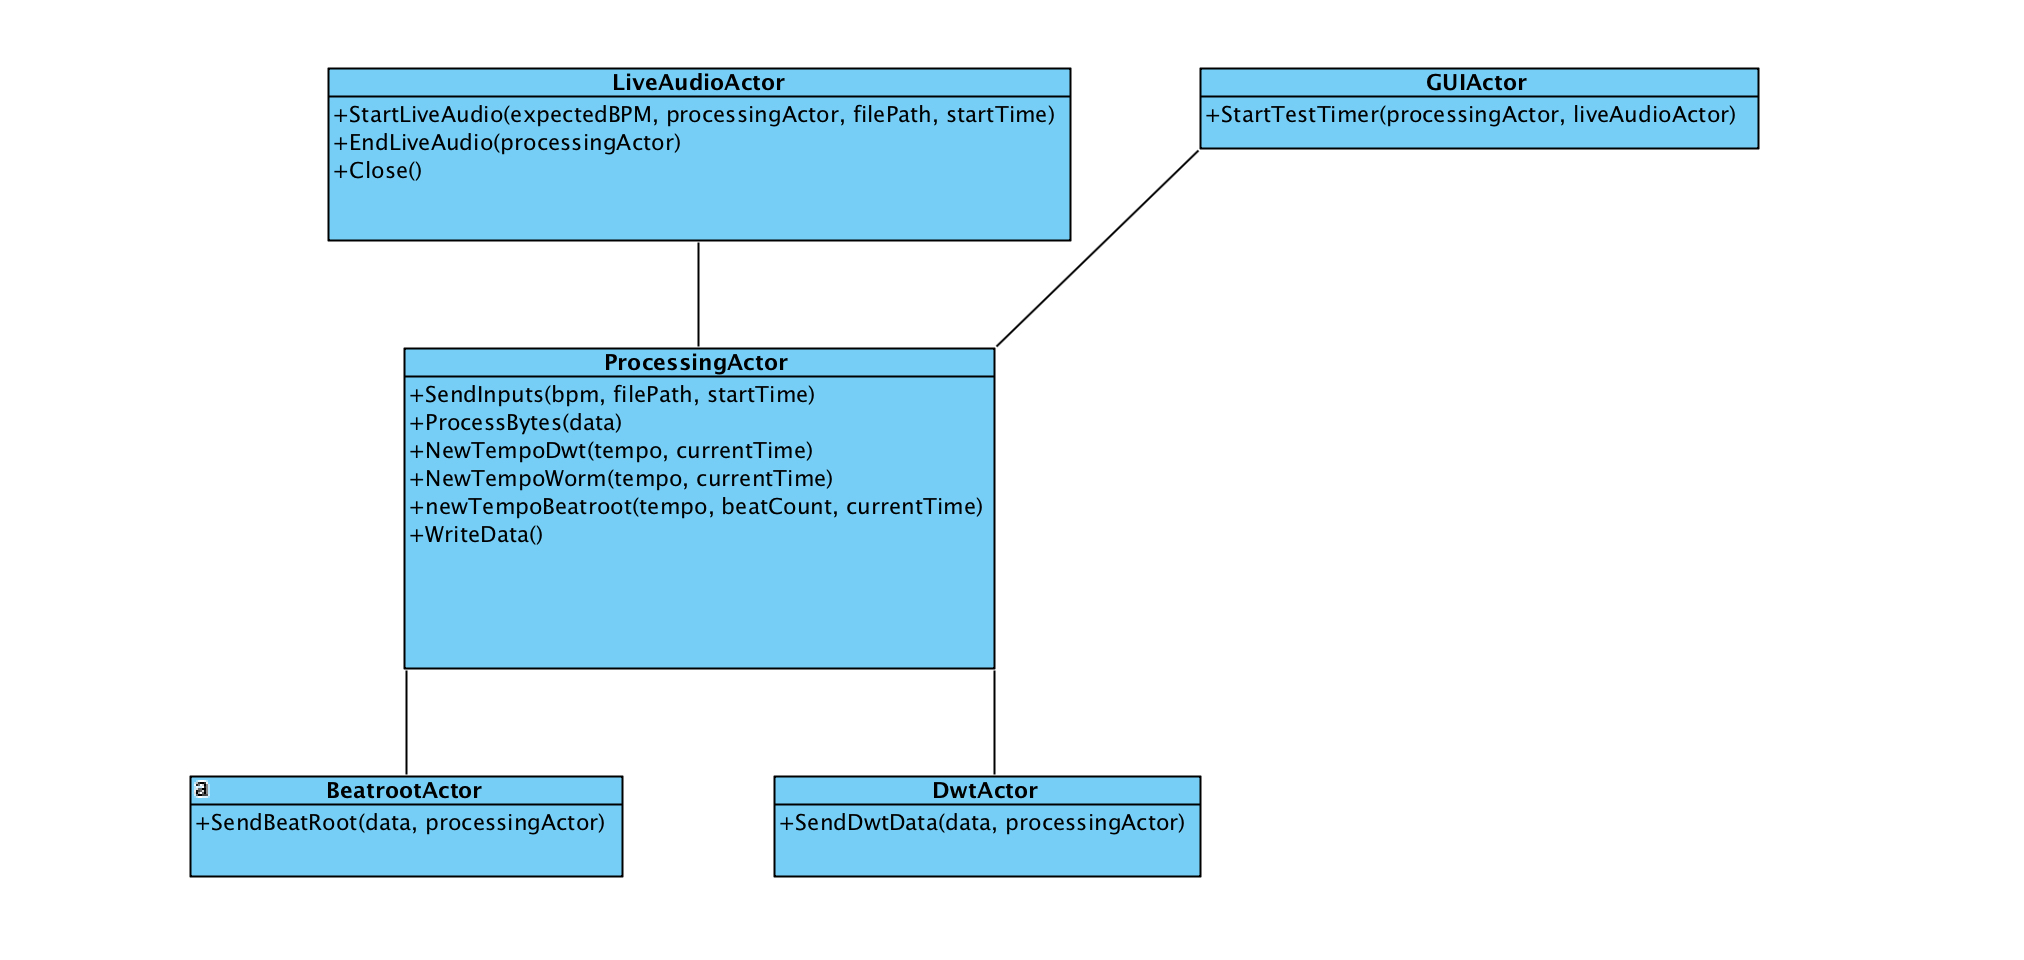
\includegraphics[scale=0.25]{images/ActorHierachy.jpg}
\caption{UML drawing of the RTT\_Analyser's actor hierachy, operations within each actor represent the messages they can recieve}
\label{fig: actorHe}
\end{figure} 

The messages permitted to be passed between the RTT\_Analyser's actors were all implemented as case classes within a sealed trait (Figure~\ref{fig: messages}). A sealed trait ensures that the only classes extending the trait are in the same file \cite{odesky}, which works well with the actor's pattern matching recieve method.\par

\begin{figure}[htbp]
\centering
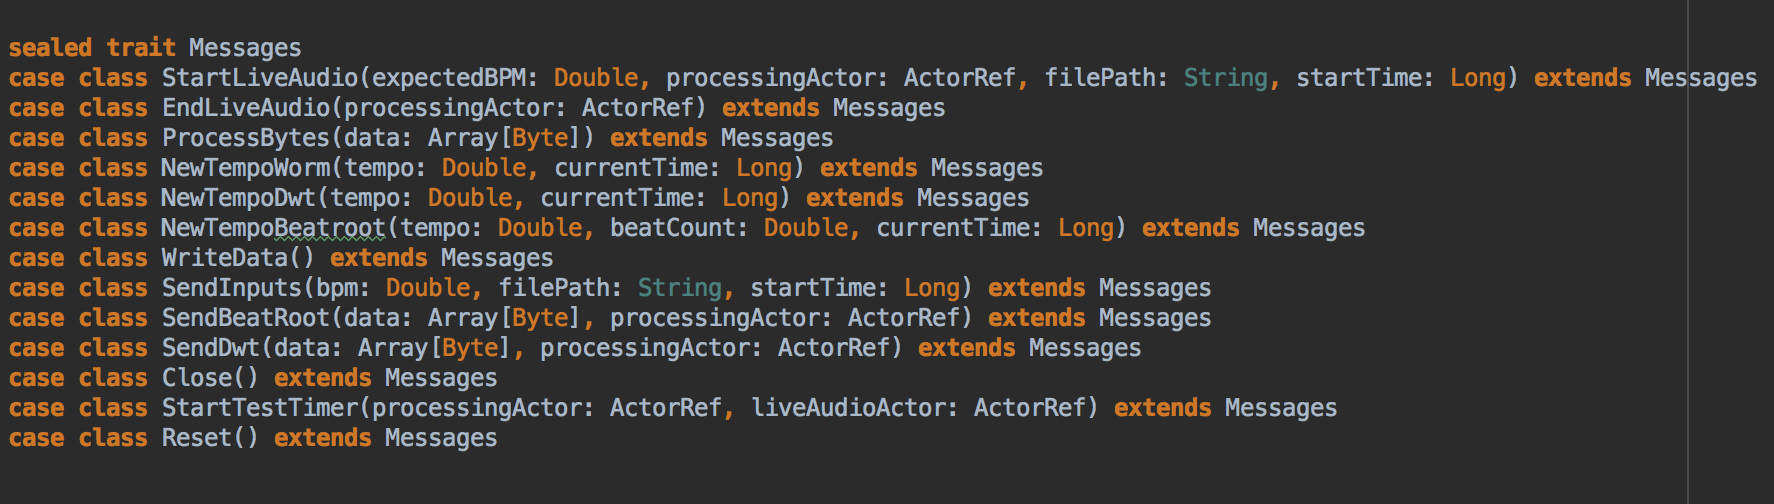
\includegraphics[scale=0.25]{images/messages.jpg}
\caption{The message case classes used by the RTT\_Analyser's actor system}
\label{fig: messages}
\end{figure} 

The \texttt{LiveAudioActor} (Figure~\ref{fig: liveaudioactor}) assumes the role of the overseer  of the system, being responsible for starting and stopping the live audio capture, as well as the termination of the RTT\_Analyser when appropriate. \par

\begin{figure}[htbp]
\centering
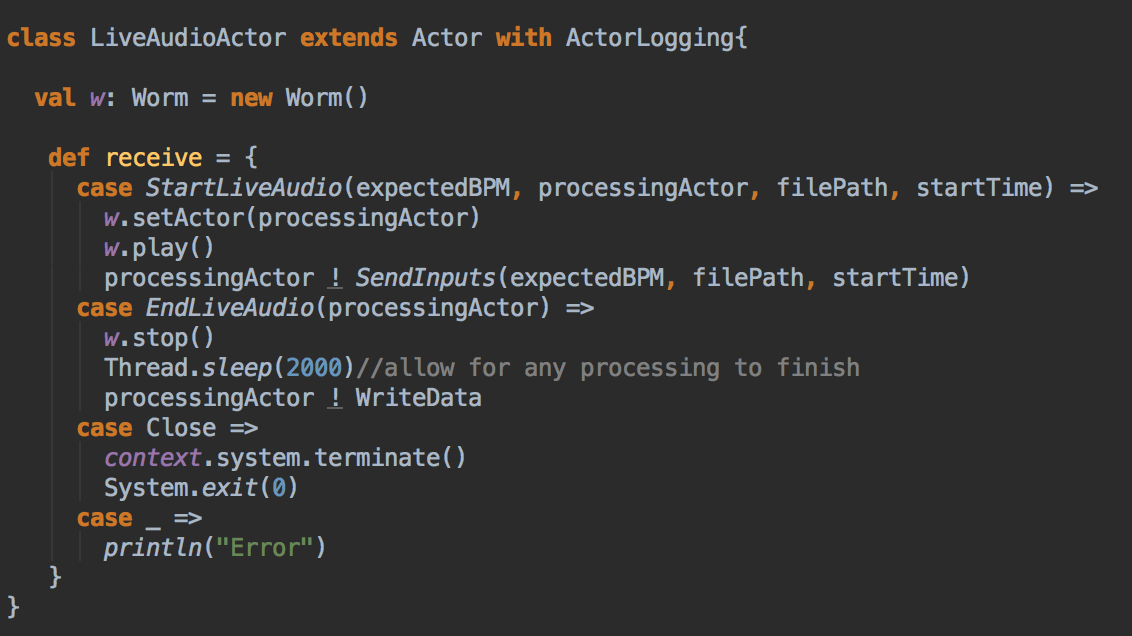
\includegraphics[scale=0.3]{images/LiveAudioActor.jpg}
\caption{LiveAudioActor class}
\label{fig: liveaudioactor}
\end{figure}

The \texttt{ProcessingActor}(Figure~\ref{fig: processingActor}), a child of the \texttt{LiveAudioActor} can be considered the coordinator of the storing and processing captured audio data, and the writing of the calculated tempos. In order to ensure the processing remains as isolated as possible the \texttt{ProcessingActor} employs two worker actors, \texttt{BeatrootActor} and \texttt{DWTActor}, carrying out the task of iniating the tempo calculation. The beat detection worker actors do not return any messages to the \texttt{ProcessingActor}, instead a reference to the \texttt{ProcessingActor}, in the form of an ActorRef handle is passed to the respective beat detection system. The calculated tempo values are then sent back directly to the \texttt{ProcessingActor} to be stored and subsequently saved to file when appropriate.\par

\begin{figure}
\centering
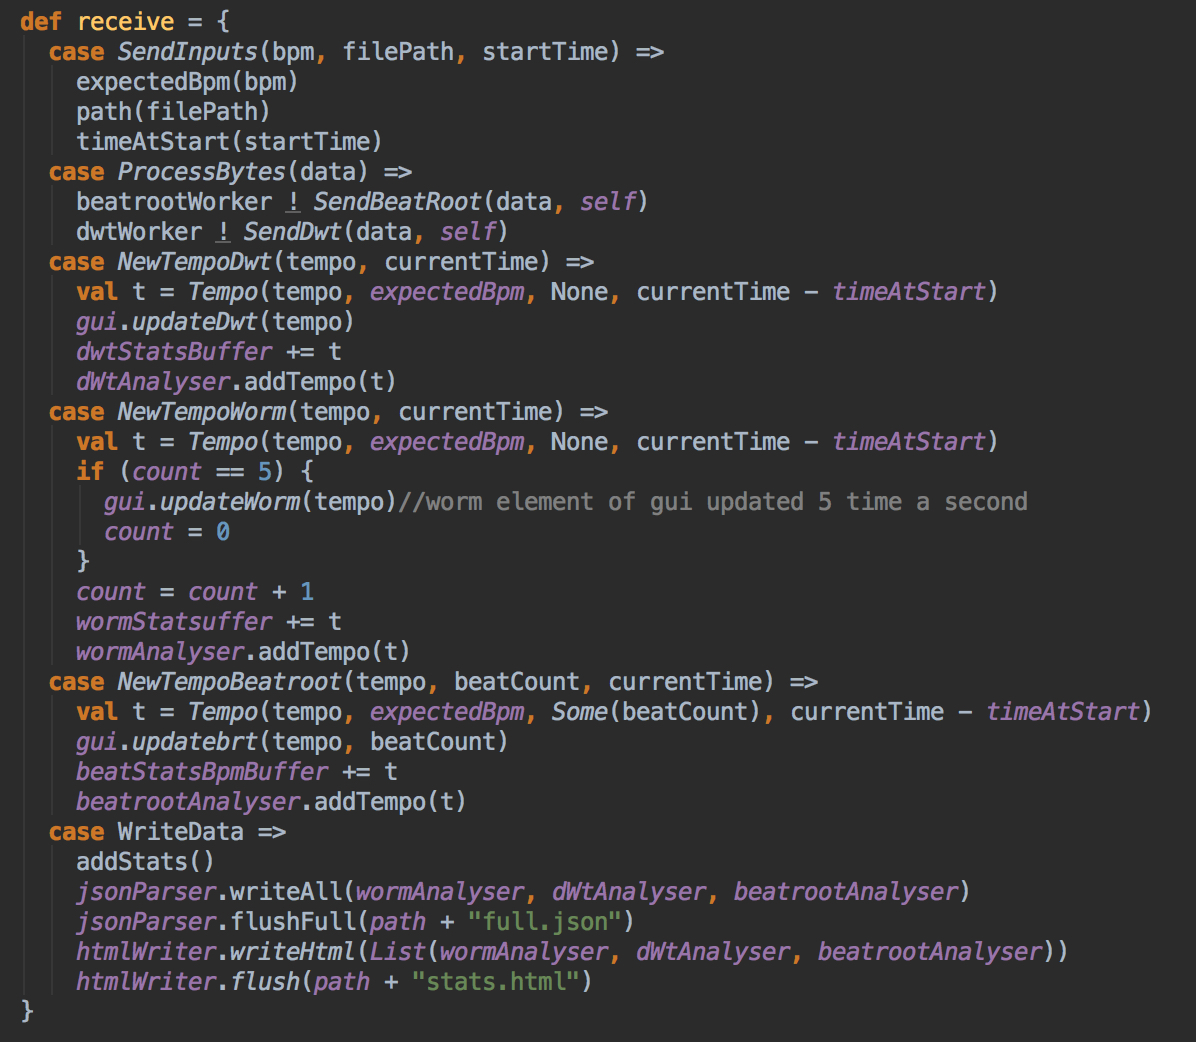
\includegraphics[scale=0.3]{images/processingRec.jpg}
\caption{Recieve method of the ProcessingActor class}
\label{fig: processingActor}
\end{figure}

The final RTT\_Analyser actor, the \texttt{GUIActor}, is a standalone actor on the same level as the \texttt{LiveAudioActor} within the actor hierarchy. the GUIActor is responsible for the timing of the beat detection test process.\par

All of the RTT\_Analyser's parent and child actors were all instantiated in the self contained \texttt{Operator} object (Figure~\ref{fig: props}. This ensured that potentially dangerous practice of declaring one actor and breaking actor encapsulation \cite{akkaActors} was avoided.  

\begin{figure}[htbp]
\centering
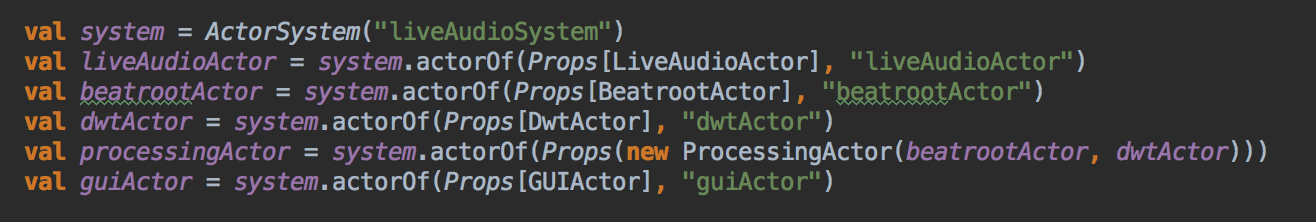
\includegraphics[scale=0.35]{images/actorprops.jpg}
\caption{Declaring of the RTT\_Analyser's actors}
\label{fig: props}
\end{figure}

\subsection{Live Audio Capture}
Originally, the RTT\_Analyser's live audio capture was handled by the \texttt{SoundCaptureImpl} class, where the raw audio was captured using the audio format described in section~\ref{sec: liveaudio}. The audio is then converted into a stream of bytes by the Java \texttt{AudioInputStream} \cite{soundTrail}, before being passed for processing by the beat detection algorithms. The sound capturing components of this class were based on those described in the Java Sound Programmer Guide \cite{javasound} and consisted of the code in Figure~\ref{fig: startcap}.

\begin{figure}[htbp]
\centering
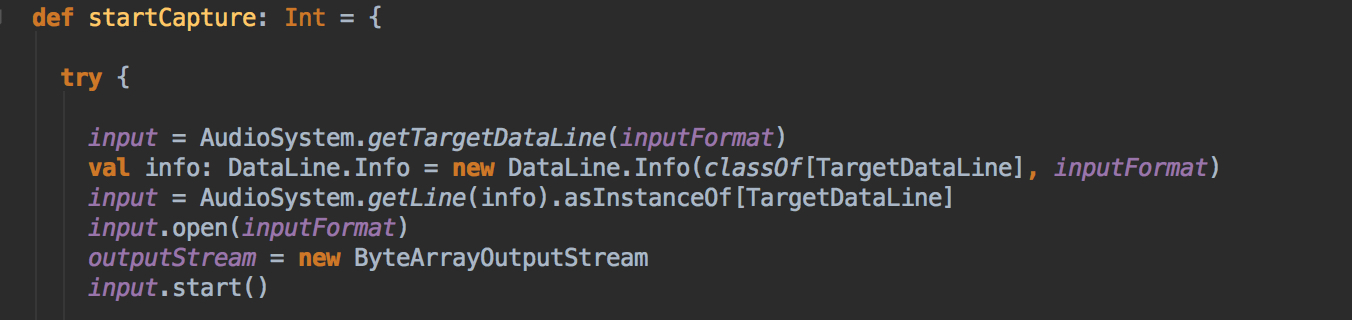
\includegraphics[scale=0.3]{images/startCap.jpg}
\caption{Example of the basis of live audio capture method in Scala}
\label{fig: startcap}
\end{figure}

The need for the code in Figure~\ref{fig: startcap} became defunct with the design decision to include the Performance Worm system within the RTT\_Analyser. As the Performance Worm is already set up to capture live audio. The captured audio now needed to be stored by the PW in a manner which allowed for all three beat detection algorithms to be able to process the same captured audio. This was achieved by adding the method \texttt{addBytes} (Figure~\ref{fig: addBytes}) to the \texttt{AudioWorm} class, responsible for the capturing and processing of the live audio within the PW. The \texttt{addBytes} method took a byte array, which was stored within a \texttt{ByteArrayOutputStream}. Once the sufficient number of bytes had been amassed the \texttt{ProcessingActor} was sent the \texttt{ProcessBytes} message, which initiated the processing of the audio data by the Beatroot and DWT beat detection systems.

\begin{figure}[ht]
	\centering
	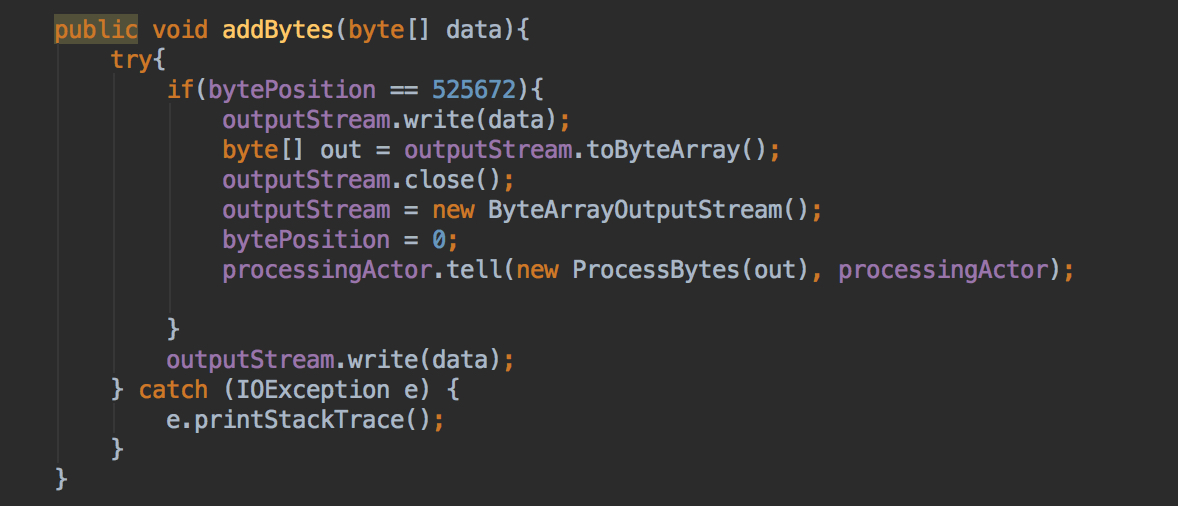
\includegraphics[scale=0.25]{images/addBytes.jpg}
	\caption{}
	\label{fig: addBytes}
\end{figure}

\subsection{DWT Beat Detection Implementation}
The DWT beat detection component of the RTT\_Analyser was originally proposed to be implemented by the author. However, due to the time spent investigating how to adapt the Beatroot system to work with live audio a different solution was needed, this was provided by the Scala implementation by Marco Ziccardi \cite{marcoZin}.

The implementation of Tzanetakis \textit{et al} beat detection algorithm by Marco Ziccardi \cite{marcoZin} was part of a larger system which offered a number of other beat detection methods. The RTT\_Analyser only required the class which implemented the DWT beat detection algorithm, \texttt{WaveletBPMDetector}, which relied on a Scala version of the WavFile Java class created by Andrew Greensted \cite{green}. However, as the RTT\_Analyser was not required to decode WAV files, this class was adapted to form the \texttt{LiveAudioProcessor} class (Figure~\ref{fig: liveAudPro}). The class was based on three methods from Andrew Greensted's WavFile class \cite{green}, \texttt{readFrames}, an overloaded \texttt{readFrames} and the \texttt{getSample} method. Rather than being simply a Scala version of the Java code, where possible these methods were written using Scala's pattern matching facility and any loops converted to a tail recursive solution.\par

The final addition to the \texttt{LiveAudioProcessor} class was the inclusion of the \texttt{addData} method, which assigns the byte array containing the raw audio to the buffer variable processed in the \texttt{getSample} method. In order for the \texttt{WaveletBPMDetector} class to return a tempo result for a single window of audio (matched to the size of the buffer byte array), the loop was removed from the bpm method. Once a tempo was calculated this was sent back to the \texttt{ProcessingActor} using the \texttt{NewTempoDWT} message.

\begin{figure}[ht]
	\centering
	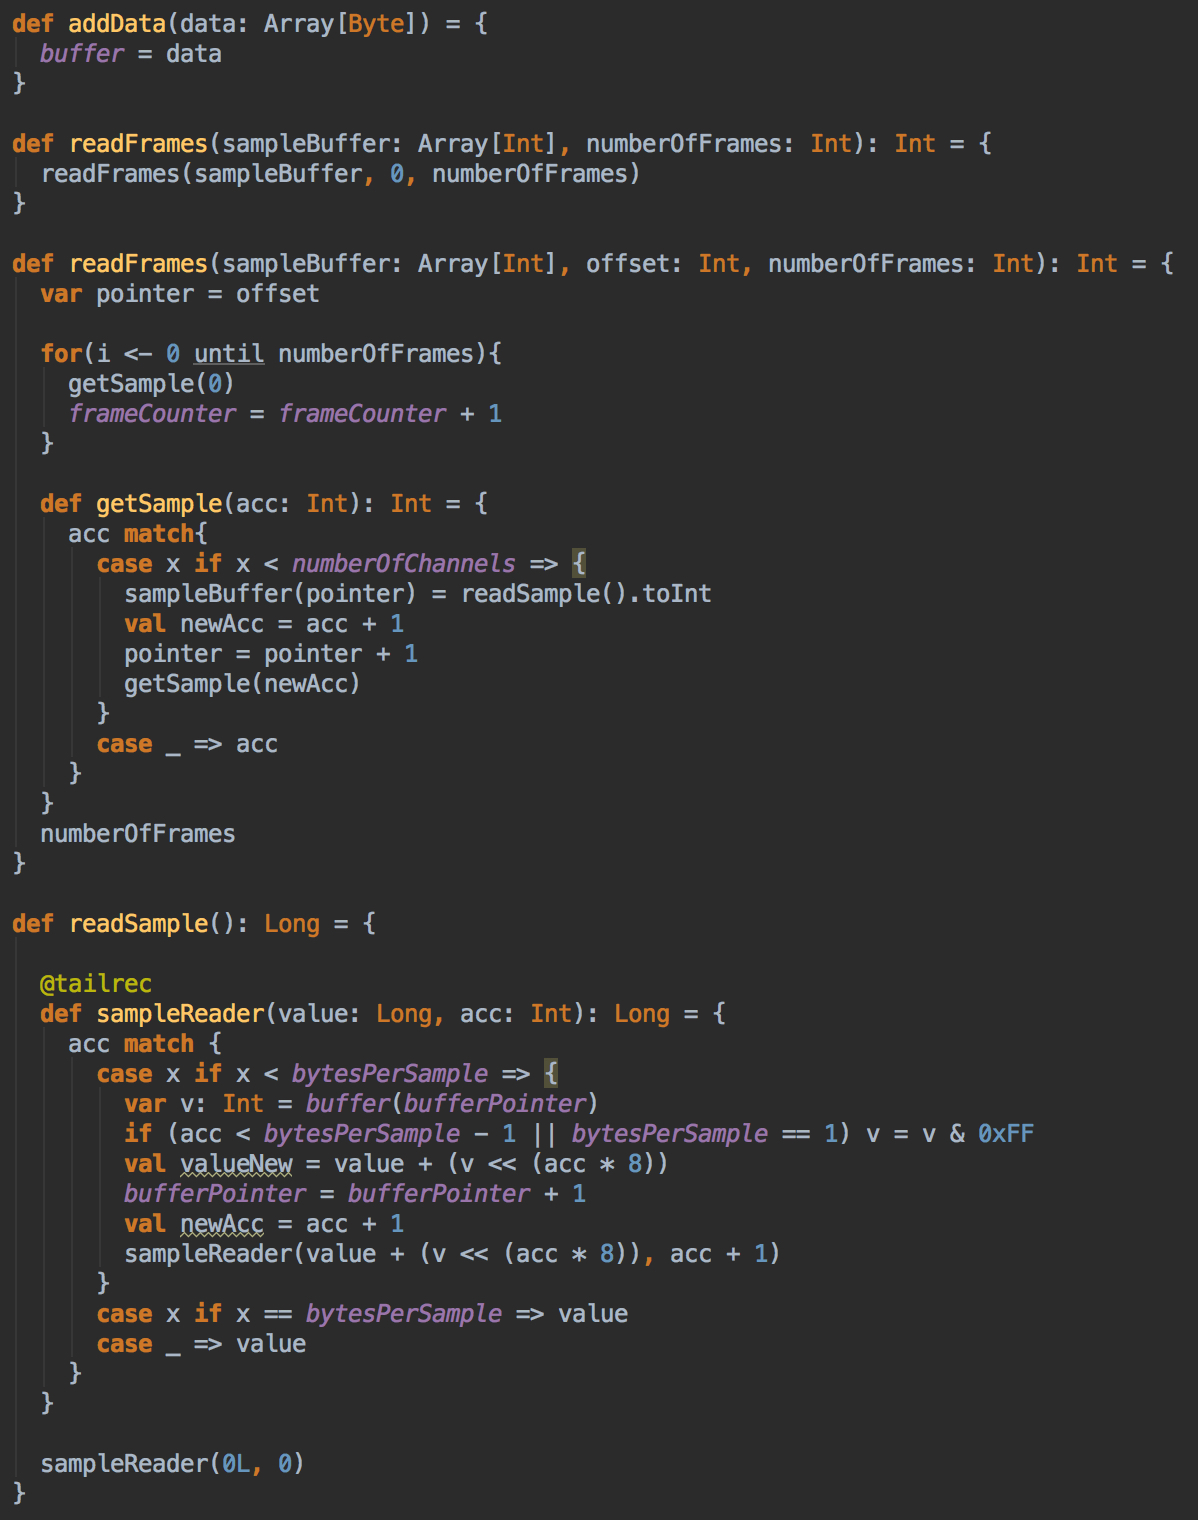
\includegraphics[scale=0.25]{images/liveAudioPro.jpg}
	\caption{LiveAudioProcessor}
	\label{fig: liveAudPro}
\end{figure}


\subsection{Tempo, Analyser and Stats}
The \texttt{Tempo} object, implemented as a method of encapsulating the RTT\_Analyser's calculated tempo results. Is Comprised of the calculated and expected tempos, and difference between these values. Additonally, an \texttt{Option}\footnote{The \texttt{Option} type is Scala's alternative to Java's \texttt{null} value, the \texttt{Option} type is in fact a container which either holds a value or is empty. It provides a much safer alternative to the error prone \texttt{null} value \cite{mariusEr}.} count of beats detected and the time at which the tempo result was calculated is included.\par 

The \texttt{Analyser} object was designed to hold the calculated \texttt{Tempo} objects within a \texttt{ListBuffer}, chosen for its scalability. The \texttt{Analyser} trait was extended to create three case classes corresponding to the relevant beat detection algorithms. The \texttt{Analyser} implementations also contained an \texttt{Option Stats} value.\par
The \texttt{Stats} object is an object used to hold the average and median values of the calculated tempos, difference between the expected and calculated tempos. The time taken to calculate a tempo within plus or minus one bpm of the expected value was also recorded in order to assess the efficiency of the beat detection algorithms. The \texttt{StatsCalculator} was a helper class responsible for carrying out computation of the values held with the \texttt{Stats} object and was implemented using the code seen in Figure~\ref{fig: statsC}.

\begin{figure}[htbp]
\centering
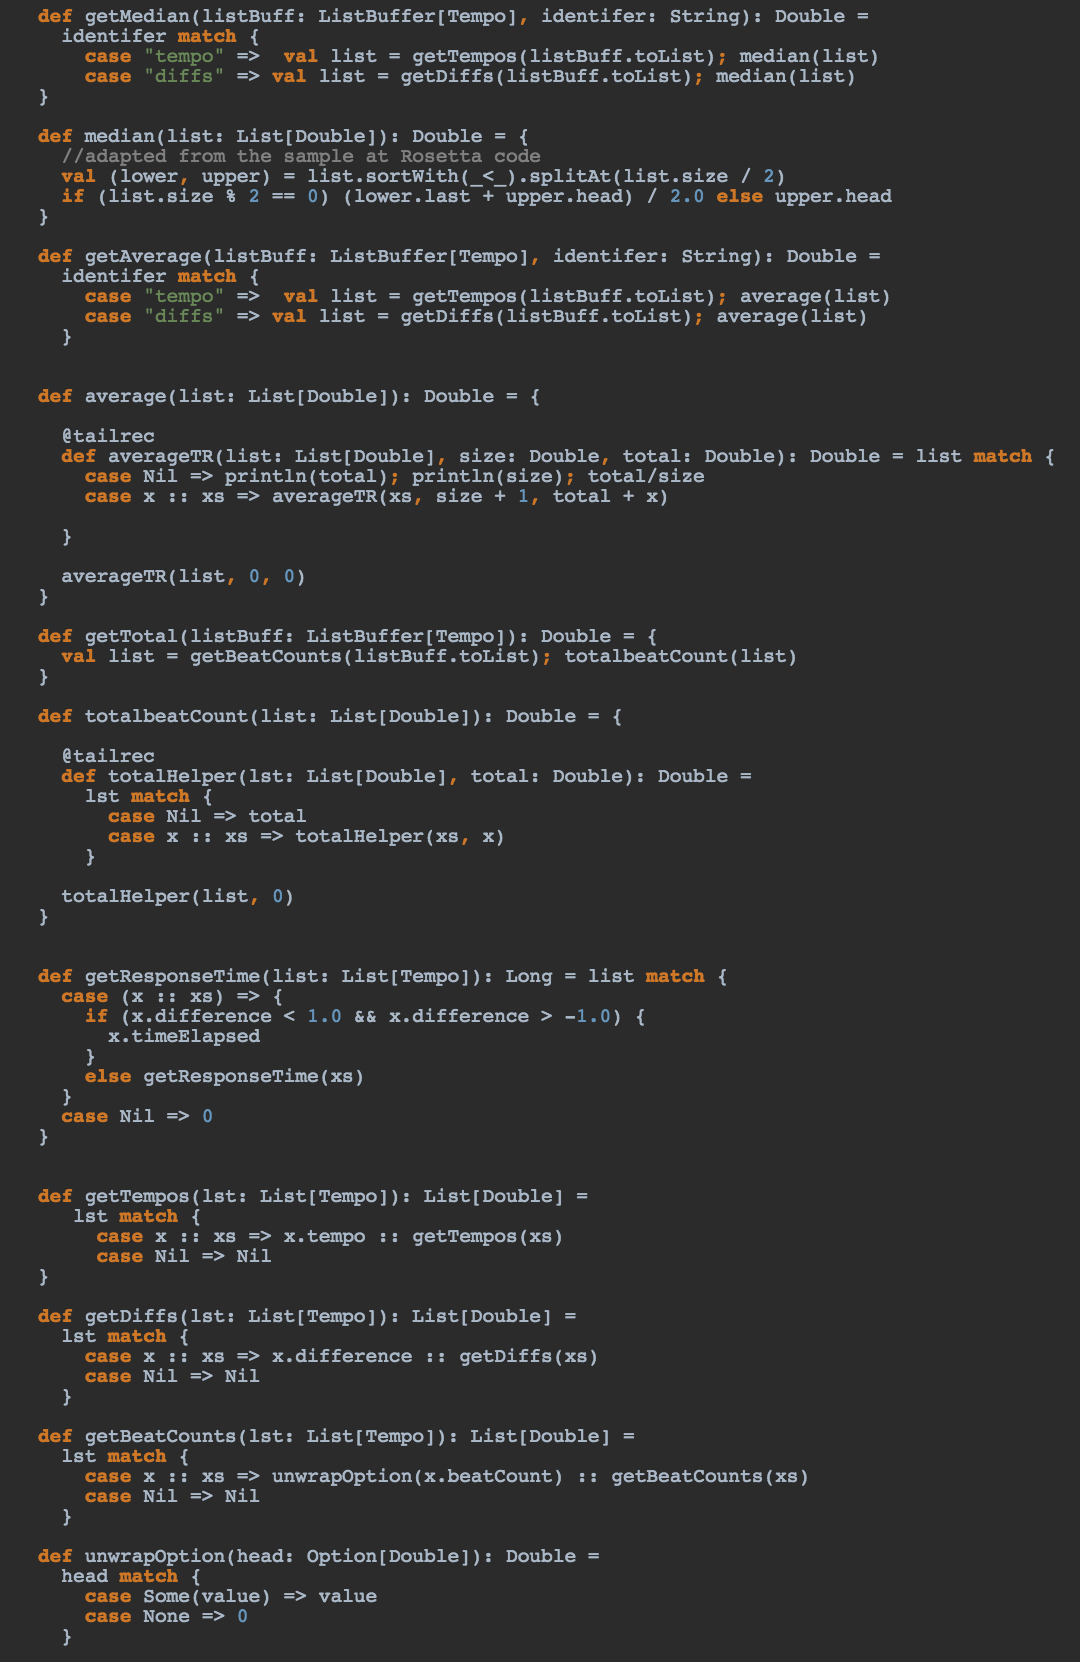
\includegraphics[scale=0.35]{images/statscalc.jpg}
\caption{Stats calculation methods used by the StatsCalculator}
\label{fig: statsC}
\end{figure}

\subsection{JSON Parsing}

The implementation of the data storage system of the RTT\_Analyser used the JavaScript Object Notation (JSON). JSON's lightweight data-interchange format \cite{json} ensured the conversion from a Scala case class to a JSON object is straightforward. The JSON is generated by the ScalaJSON library provided by the play framework \cite{play}. Specifically the \texttt{Writes} object, which converts an object into a JSON representation. Three methods were written in order to account for the three implementations of the \texttt{Analyser} trait, an example of the code can be seen in Figure~\ref{fig: json}.\par

As JSON is written in a text format \cite{json}, the parsing of generated JSON was performed by simpling converting the JSON objects generated by the respective \texttt{write} methods to a string. This was then written to a JSON file where the path was provided from the user interaction with the RTT\_Analyser's user interface.

\begin{figure}[htbp]
\centering
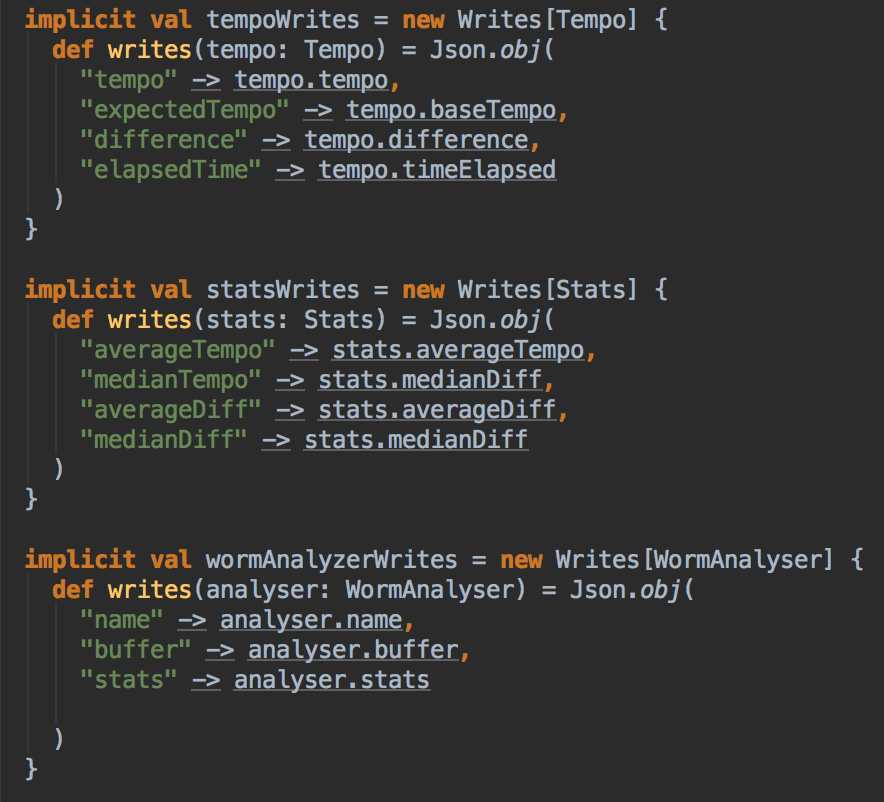
\includegraphics[scale=0.25]{images/writes.jpg}
\caption{Example of the write method used to convert the Tempo and Stats object values to JSON}
\label{fig: json}
\end{figure}

\subsection{Adaption of Beatroot}
Once the development of the RTT\_Analyser was considered to be sufficiently on schedule, the adaption of the Beatroot system to work with live audio was attempted again. As with the \texttt{WaveletBPMDetector}, Beatroot would have to be set up to use the same audio bytes as those captured by the PW. As the PW's \texttt{AudioWorm} class was already set up to capture the enough bytes to work with the \texttt{WaveletBPMDetector}'s smallest working window size of 131072, the same figure was chosen to be processed by Beatroot. \par

With the correct design decisions now taken the live audio adaption of Beatroot consisted of only a few minor steps. First, the \texttt{processFile} method was amended to receive the byte array holding the audio data recorded by the Performance Worm. A \texttt{ByteArrayInputStream} was then instantiated to hold the data, allowing the \texttt{processFrame} and \texttt{getFrame} methods to work in the same manner as with a static audio file. After the captured audio was processed the \texttt{ByteArrayInputStream} was closed, a step necessary to ensure that no overlap existed between captured audio data sets sent to be processed.

\subsection{RTT\_Analyser User Interface and HTML Results Viewer}
The RTT\_Analyser's user interface (Figure~\ref{fig: rtt}) was designed with simplicity in mind and was implemented using the ScalaFX\cite{scalafx}. Sitting on the top of the JavaFX API and using the same declaration syntax as normal objects within Scala, ScalaFX enables developers to use the same syntax to create and modify the user interface's scene graph\footnote{A hierarchy of tree nodes what represent the visual components of an application's user interface\cite{oracle2}} \cite{scalafx}. \par

Before the user could begin live audio capture, the expected bpm, file name and path were required. Once input, there are two modes available to the user. The first is to control the live audio beat detection manually using the start and stop buttons accordingly. The second, is the test mode that runs the audio capture and beat detection for thirty seconds, before closing down audio inputs and storing the results. During execution in both modes the RTT\_Analyser displays the calculated tempo values to the user as a bpm value rounded to two decimal places. \par

\begin{figure}[htbp]
\centering
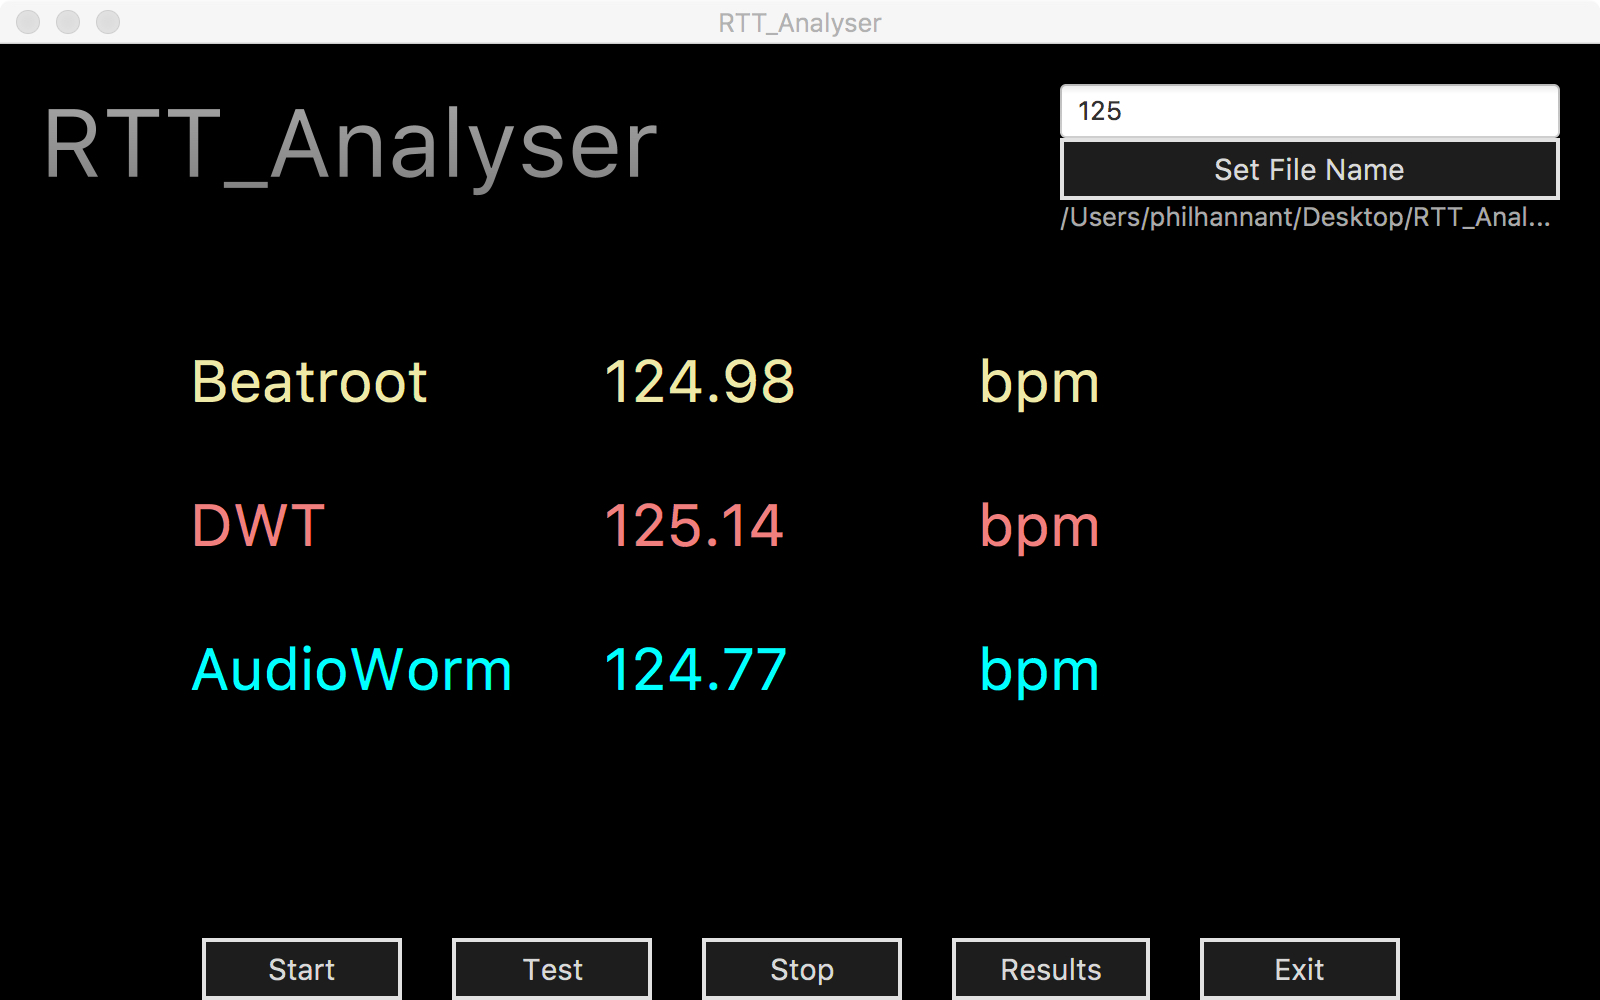
\includegraphics[scale=0.25]{images/rtt.jpg}
\caption{RTT\_Analyser's User Interface}
\label{fig: rtt}
\end{figure}

On completion within both modes the results are stored within a JSON file automatically and also written to an HTML file. The results can then be viewed in a web browser using the \textit{Results} button. The HTML tables were produced in \texttt{HtmlWriter} object which used reflection where possible to obtain the relevant field names, before using a number of tail recursive methods to write the field values and HTML tags to a \texttt{StringBuilder} object, chosen for it's mutability. The HTML tables are subsequently saved to an HTML file which is opened and viewed via the default browser. An example of the displayed results can be seen in Figure~\ref{fig: htmlView}.

\begin{figure}[htbp]
\centering
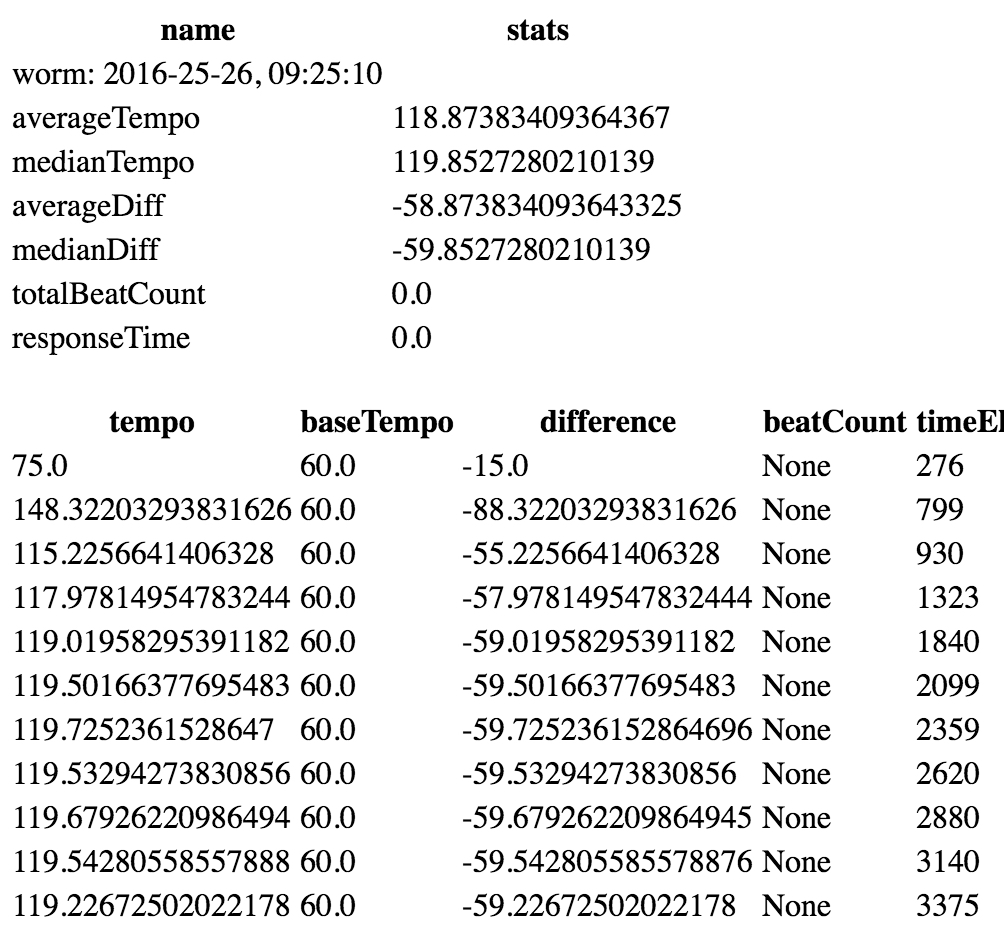
\includegraphics[scale=0.3]{images/htmlResults.jpg}
\caption{Example of the RTT\_Analyser's HTML results view}
\label{fig: htmlView}
\end{figure}

\maketitle{}\section{Software Testing}
During the development of the RTT\_Analyser, Test Driven Development (TDD) was employed where possible. TDD is a development process that uses test-first development and refactoring. Test-first development involves writing a test before just enough production code is written to pass that test \cite{tdd1}. Refactoring is the process of making small changes to code and is used to improve the design of the code. Thus, making it easier to understand and modify \cite{tdd2}. \par

The tests were written using the ScalaTest framework, which is one of the most dominant Scala testing frameworks currently available. ScalaTest is designed with the intention of providing a test framework that makes testing more concise and uses the Scala language in a way to ensure testing is easy and fun \cite{testingScala}.

TDD was used at any stage of the development process where a piece of code with an expected behaviour was being implemented. It was not used for all classes, as when dealing with live audio it was not possible to know the exact data that would be recorded due to the presence of background noise. Although, where the requirement was simply to return a value of a certain type, basic TDD tests were written. The classes that were ideally suited to TDD and were developed completely using it were the Tempo, Analyser implementations, StatsCalculator, JSONParser and HTMLWriter. \par

A good example of TDD being applied during the development of the RTT\_Analyser was during the creation of the StatsCalculator. Designed to carry out average and median calculations on the stored Tempo objects held within the Analyser implementations enabled TDD to be employed successfully.

When it was not possible to use TDD, particularly during the initial set-up and testing of the beat detection algorithms with live audio. A simpler testing approach was taken, consisting of running the system with a selection of sample drum beats of varying tempos, with console logs used to test that the system was performing the desired tempo calculations.

\maketitle{}\section{RTT\_Analyser Beat Detection Testing}
\subsection{Drum Beat Sample Set}
Once the software testing of the RTT\_Analyser was complete, the full testing process could begin. The sample drum beats were written using the Apple sequencer program, GarageBand \cite{garage}. The writing of the drum beats took a slight deviation from the project proposal, rather than create multiple full drum beats in a varying number of styles, the drum beats were instead tested in layers. For example, a simple four four (4/4) bass drum beat with a back beat and the time element being played on the hi-hat cymbal would account for four samples. This decision stemmed from how a cymbal behaves when it is played at high amplitudes (loudness), the vibrations it create become chaotic and its clearly identifiable signals disappear, effectively becoming noise \cite{soundonsound}. Therefore, to compare the drum samples with cymbals a baseline was required. This change was also considered to help provide a much more diverse data set, hopefully helping the understanding of how the different elements of a drum kit, not just cymbals, can affect the accuracy of the beat detection algorithms being tested by the RTT\_Analyser.\par

Additonally, three Garageband stock samples were added to the sample set. These samples were included in an attempt to provide insight as to whether the beat detection algorithms are able to work efficiently, even when drum beat being tested is fairly complex.

In total, twenty eight drum samples were produced and the full details of the elements which each drum beat was comprised of and style of the drum beat can be seen in Table~\ref{tab: beats}. A full visualisation of the drum beats used can be found in Appendix A.

\subsection{Real Time Tempo Tests}
The real time tempo detection tests were carried out in an environment with as little background noise as possible. The drum beats were played on an external speaker set to the same volume for all tests. Each drum beat was tested for thirty seconds over the tempo range of 60-160 bpm, where the tempo was increased in five bpm increments. Resulting in twenty one tests being carried out for each drum beat, producing a sample set consisting of 588 results files.

During the real time tempo tests it became apparent that at lower tempos the RTT\_Analyser was returning values which were roughly twice that of the expected tempo. A possible explanantion for this was considered to be aliasing. Resulting in it not being possible to distinguish between the values from sampled audio as they contain periodic replications of the original spectrum\cite{lyons}. As this behaviour was being displayed by all three of the beat detection algorithms. It was decided that all of the drum samples would be reprocessed through the RTT\_Analyser. However, this time a low-pass filter would applied to the point at which the audio is captured. The low-pass filter was provided by the source\_code.biz Java dsp collection and the cutoff frequency was set to 100 Hz.
\clearpage

\begin{table}[htbp]
\vspace{-1in}
\caption{List of Drum Beats Used in RTT\_Analyser Tests} 
\centering
\scalebox{0.75}{
\begin{tabular}{|p{3cm}|p{4cm}|l|}
\hline
\textbf{Drum Beat Code} & \textbf{Elements} & \textbf{Style} \\ [0.5ex]
\hline 
AMPEDUP & All & Heavy rock, GarageBand stock drum beat\\
\hline 
HT & High tom-tom & Straight\\
\hline 
HTLT & High tom-tom and low tom-tom & Straight\\
\hline 
HTLT2 & High tom-tom and low tom-tom & Straight\\
\hline 
K & Bass drum & Straight\\
\hline 
KS & Bass drum and snare drum & Straight\\
\hline 
KS2 & Bass drum and snare drum & Straight\\
\hline 
KSCR & Bass drum, snare drum and crash cymbal & Straight\\
\hline 
KSFTTF & Bass drum (four to the floor) and snare drum & Straight\\
\hline 
KSH & Bass drum, snare drum and hi-hat cymbal & Straight\\
\hline 
KSH2 & Bass drum, snare drum and hi-hat cymbal & Straight\\
\hline 
KSH2CR & Bass drum, snare drum, hi-hat and crash cymbals & Straight\\
\hline 
KSHCR & Bass drum, snare drum, hi-hat and crash cymbals & Straight\\
\hline 
KSHHTLT & Bass drum, snare drum, hi-hat cymbal, high tom-tom and low tom-tom & Straight\\
\hline 
LT & Low tom-tom & Straight\\
\hline 
MTREVIS & All & Mowtown swing, GarageBand stock drum beat\\
\hline 
OFF-KSH & Bass drum, snare drum and hi-hat cymbal & Offbeat played on hi-hat\\
\hline 
OFF-KSHCRFTTF & Bass drum (four to the floor), snare drum, hi-hat and crash cymbals & Offbeat played on hi-hat\\
\hline 
OFF-KSHFTTF & Bass drum (four to the floor), snare drum, hi-hat cymbal & Offbeat played on hi-hat\\
\hline 
OFF-KSHHCRFTTF & Bass drum (four to the floor), snare drum, hi-hat and crash cymbals & Offbeat played on hi-hat\\
\hline 
S & Snare drum & Straight\\
\hline 
SMASH & All & Punk rock (loud), GarageBand stock drum beat\\
\hline 
SW-H & Hi-hat cymbal & Swing\\
\hline 
SW-K & Bass drum & Swing\\
\hline 
SW-KH & Bass drum and hi-hat cymbal & Swing\\
\hline 
SW-KS & Bass drum and snare drum & Swing\\
\hline 
SW-KSH & Bass drum, snare drum and hi-hat cymbal & Swing\\
\hline 
SW-R & Ride cymbal & Swing\\
\hline 
SW-SH & Snare drum and hi-hat cymbal & Swing\\
\hline
\end{tabular}}
\label{tab: beats}
\end{table}
\clearpage
\maketitle \section{Results}
The twenty eight sample beats processed by the RTT\_Analyser yielded 137,180 separate tempo records. A breakdown of the number of tempo records recorded per beat detection algorithm can be seen in Figure~\ref{fig: totrec}. The separate JSON files were then consolidated into one file, converted into a CSV file and connected to the data visualisation software package, Tableau\cite{tableau}.

\begin{figure}[htbp]
\centering
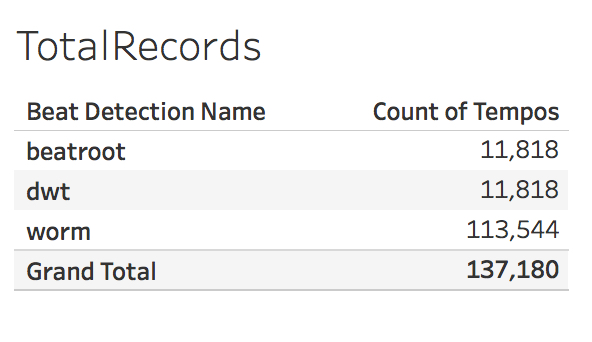
\includegraphics[scale=0.3]{totRec.jpg}
\caption{Total number of tempo values recorded by the RTT\_Analyser}
\label{fig: totrec}
\end{figure}

\subsection{Overall Average Difference}
The difference between the expected tempo and the calculated tempo was determined by subtracting the calculated tempo from the expected tempo (~\ref{eq: diff}). If the difference is negative then the calculated tempo was greater than expected and if a positive difference was returned the tempo was less than the expected value.

\begin{equation}\label{eq: diff}
\begin{split}
difference& =expected tempo - calculated tempo\\
\end{split}
\end{equation}

The average difference for each of the three beat detection algorithms, split by style can be seen in Figure~\ref{fig: aveDiff}. The best performing beat detection method can be seen to be the DWT based algorithm by Tzanetakis \textit{et al}'s \cite{tzane1}, for the samples without a filter in a Swing style. As mentioned previously, during the testing process some of the tempo results returned were double that of the expected bpm value, possibly due to aliasing. A solution to the aliasing issue, hereafter referred to as doubling, was to add a low-pass filter and looking at the results on the whole it can be considered to have worked to a certain degree. For six out of the nine sets of results, those samples processed with a low-pass filter produced a lower average difference than those without a filter. Although, the margin of error between the expected tempo and the calculated tempo are still suitably large.\par

\begin{figure}[htbp]
\centering
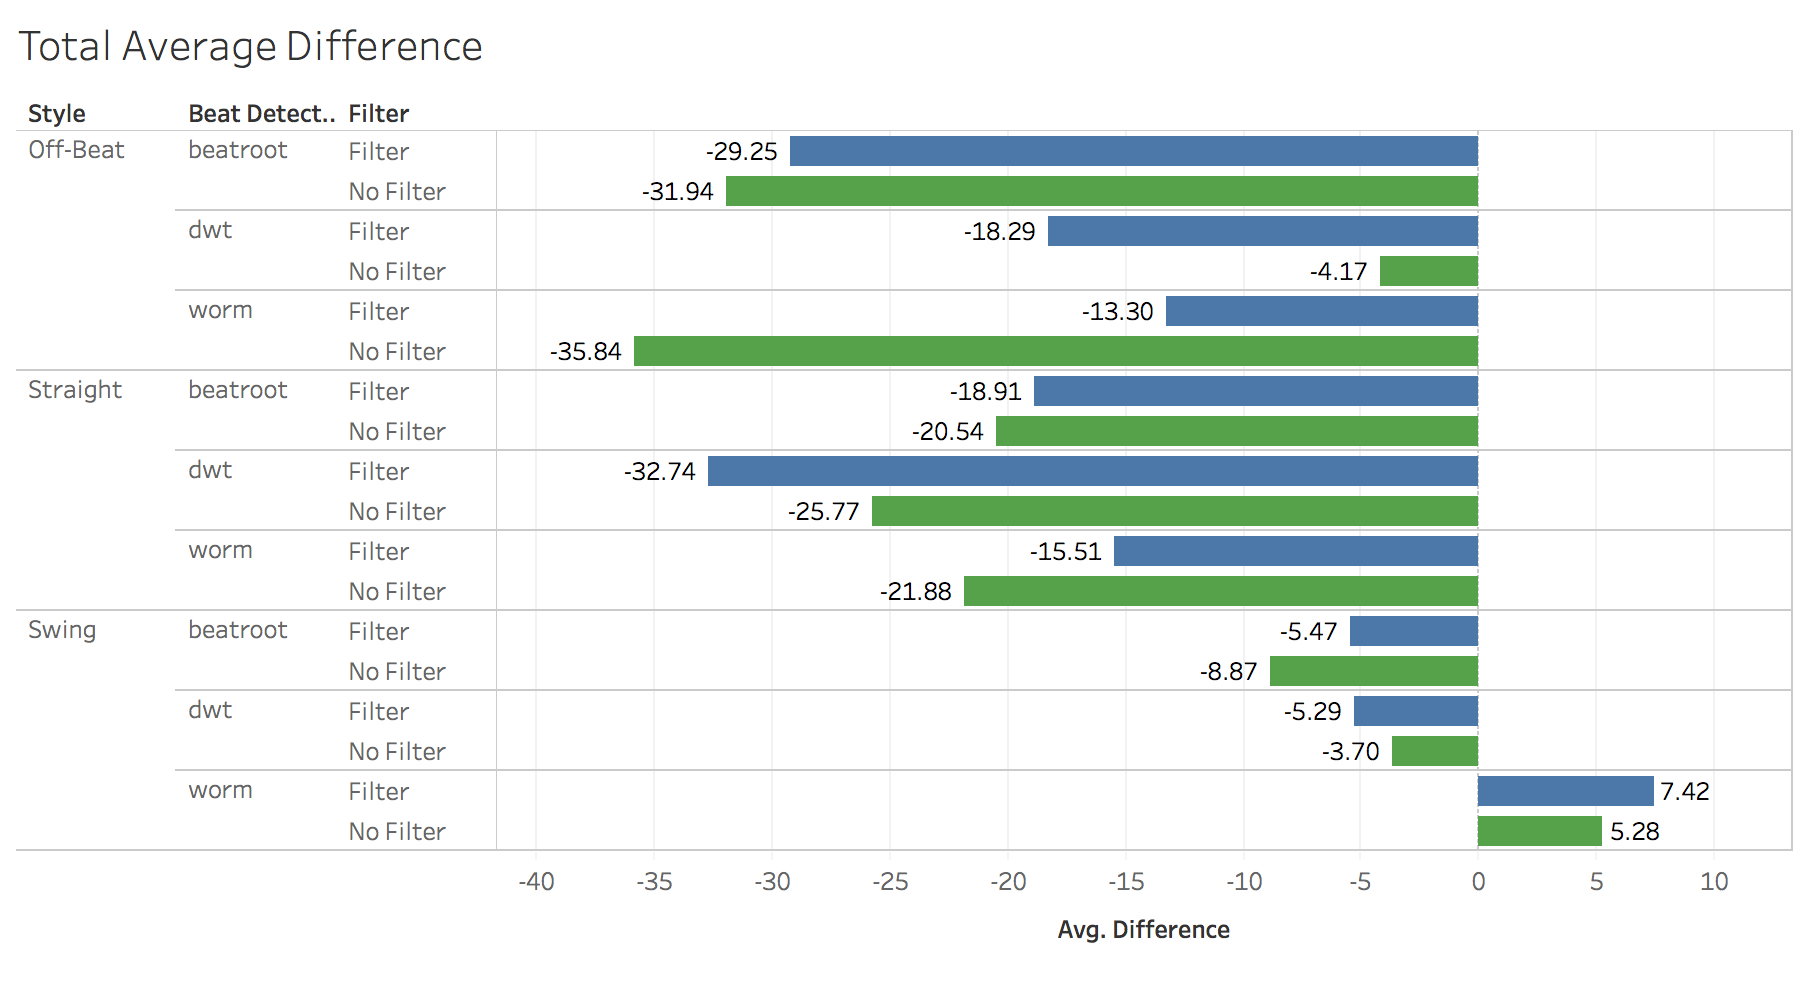
\includegraphics[scale=0.25]{images/totAveDiff.jpg}
\caption{Total average difference results}
\label{fig: aveDiff}
\end{figure}

A flag was then applied to the results set to highlight any tempo result approximately double the expected value. A record was flagged, if the calculated tempo when divided by the expected tempo returned a result greater or equal to 1.95 (~\ref{eq: flag}). The flagged results were then filtered out of the data set and the updated results can be see in Figure~\ref{fig: upAveDiff}. With the flagged results removed the average difference value for all of the beat detection algorithms was greatly reduced except for the swing samples processed by the PW. 

\begin{equation}\label{eq: flag}
\begin{split}
Calculated Tempo/Expected Tempo >= 1.95\\
\end{split}
\end{equation}

\begin{figure}[htbp]
\centering
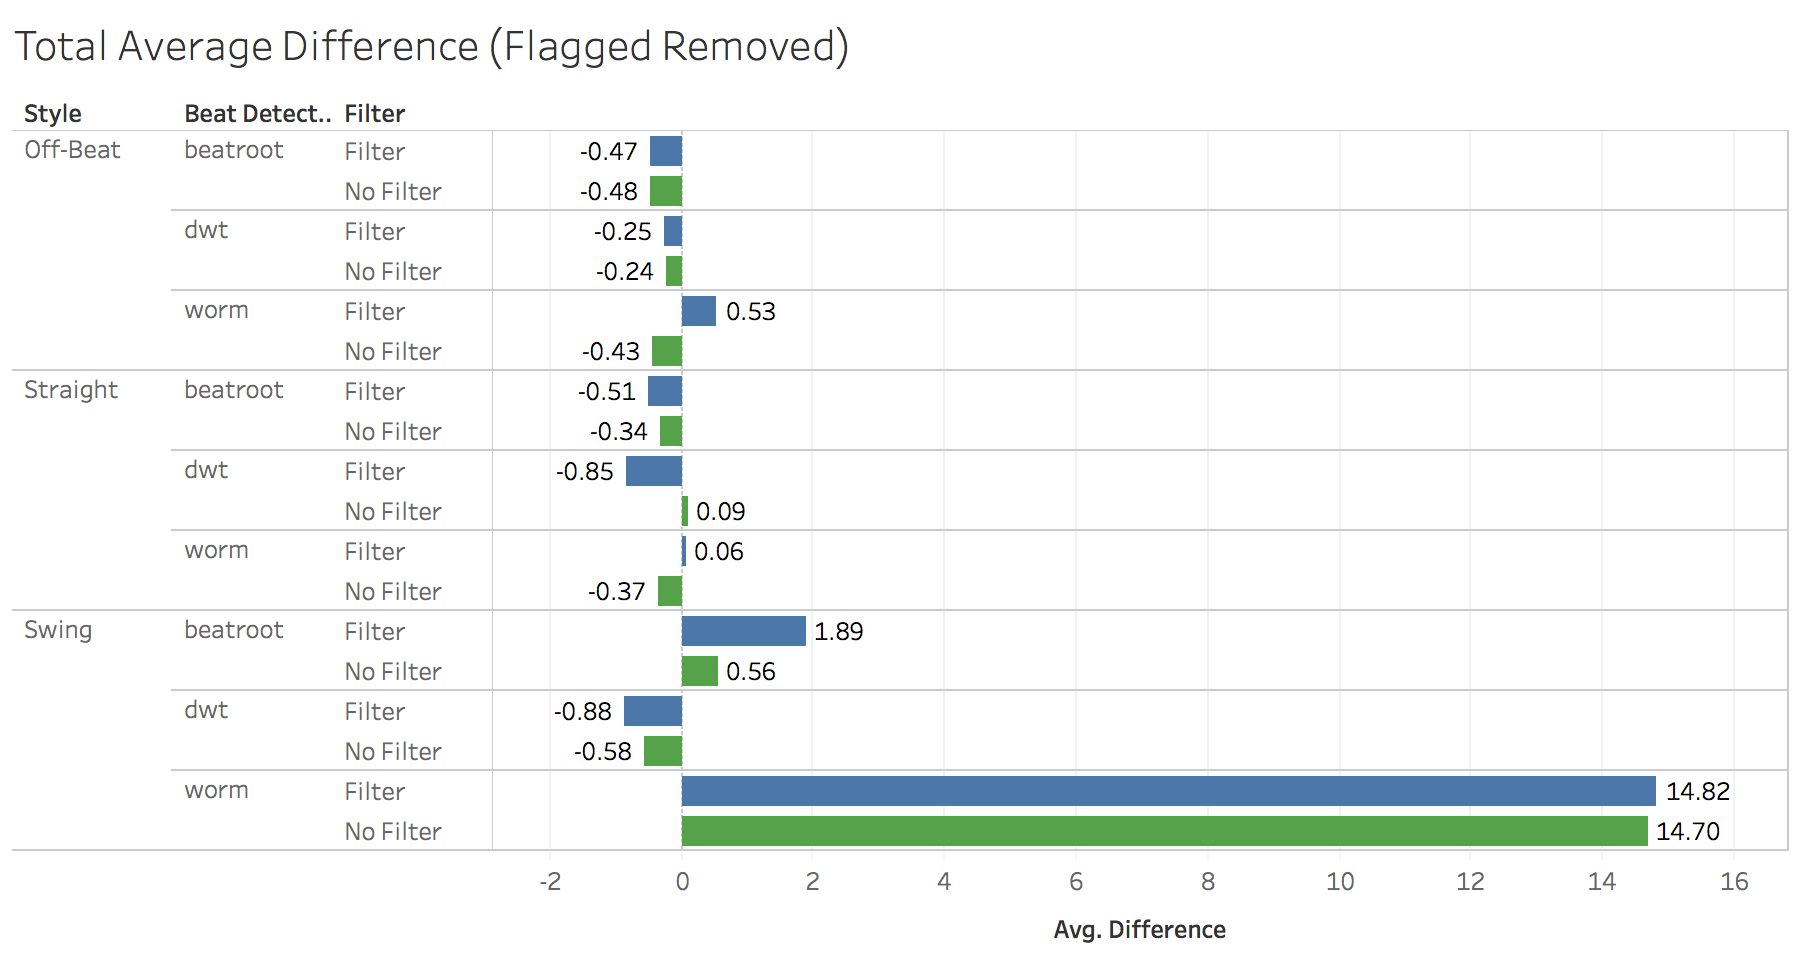
\includegraphics[scale=0.25]{images/totAveDiffFR.jpg}
\caption{Total average difference results with flagged values removed}
\label{fig: upAveDiff}
\end{figure}

Rather than just removing these results altogether, the next step was to attempt to correct any of the flagged tempo results that when divided by two, were within plus or minus five percent of the expected tempo result. With this adaption applied to the data set (seen in Figure~\ref{fig: corAveDiff}), it is clear that overall the Tzanetakis \textit{et al}'s \cite{tzane1} DWT method is the most accurate. The different musical styles within the samples also affect the accuracy of the calculated tempos. With the swing samples producing the least accurate results for all three algorithms.


\begin{figure}[htbp]
\centering
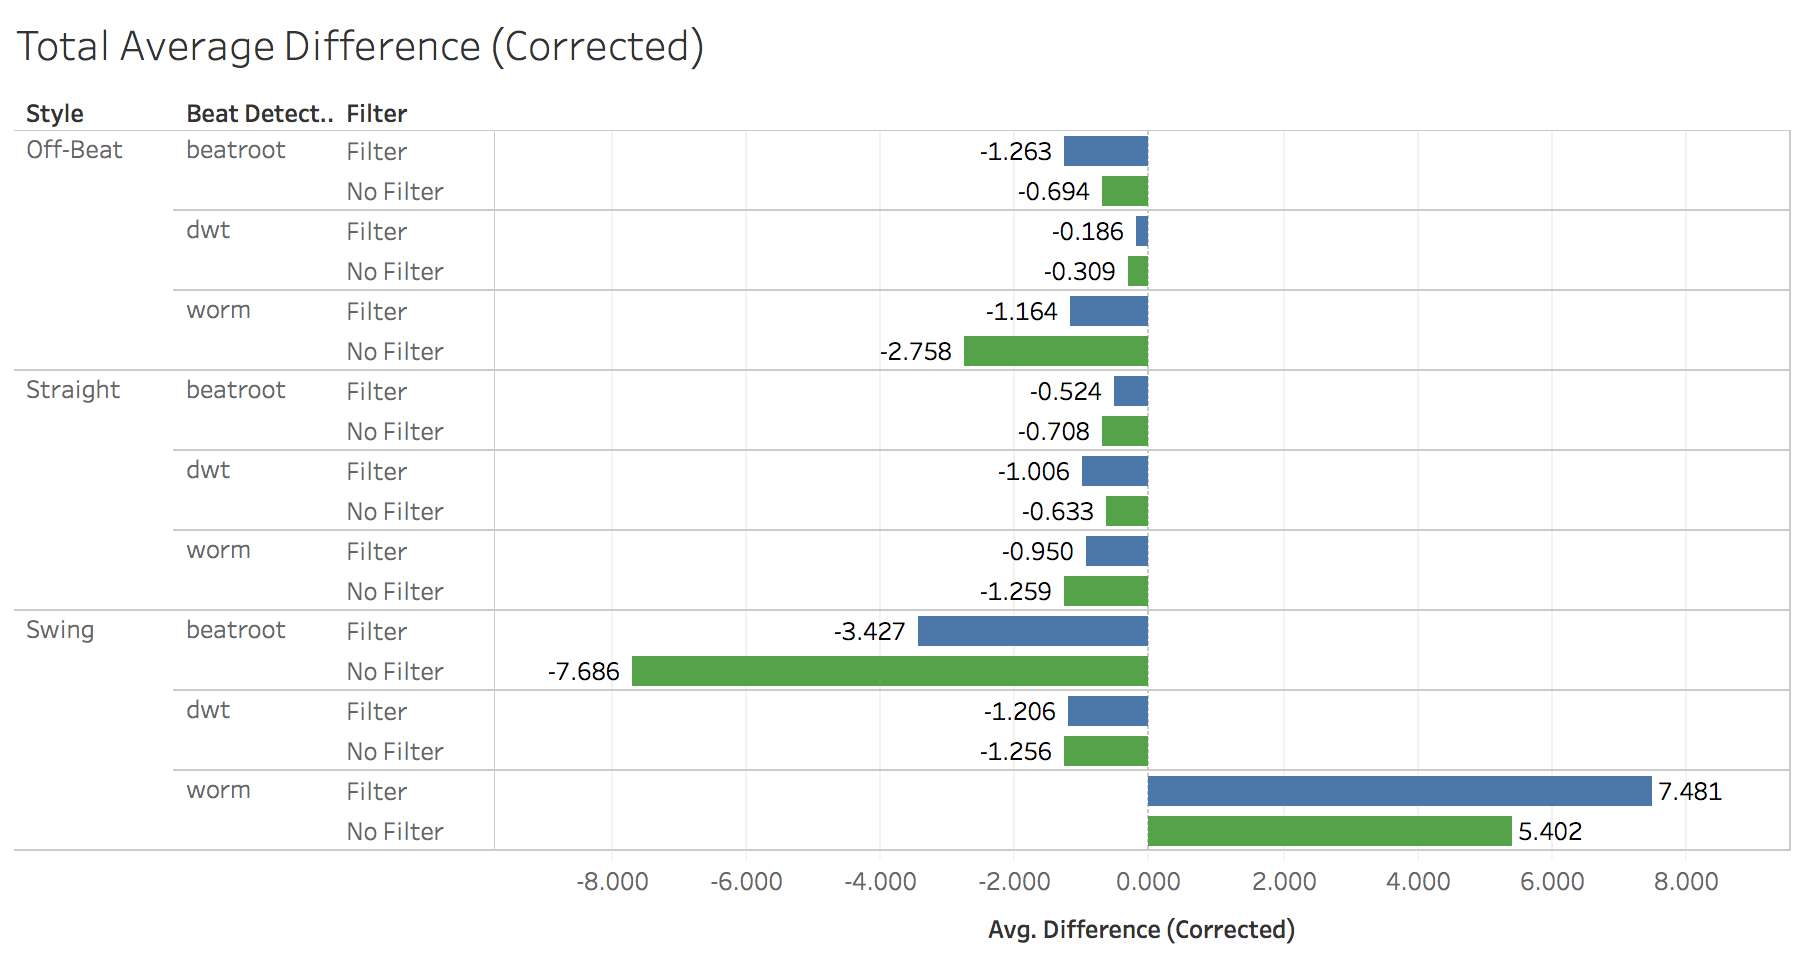
\includegraphics[scale=0.25]{images/totAveDiffCor.jpg}
\caption{Total average difference results with correction applied}
\label{fig: corAveDiff}
\end{figure}

% All of the average difference values used from this point use the original and corrected values described in the previous section. Versions of the flagged results can be found in Appendix...

% \subsection{Single Drum Sample Results}
% The next data set consists of any samples which were played using only one drum. All of the samples except for the HT (high tom-tom) and LT (low tom-tom) in the straight sample set were used as parts in the final complete drum patterns.\par

% \subsubsection{Straight Single Drum Sample Results}

% The straight single drum result set can be seen in Figure~\ref{fig: ssdAveDiff}, again the Tzanetakis \textit{et al}'s \cite{tzane1} DWT method calculated tempos with the highest level of accuracy. Performing the best for three of the four sample sets, although actually returning the lowest level of accuracy of the three beat detection methods the for the hi-hat sample.\par

% \begin{figure}
% \caption{Straight Single Drum Average Diff}
% \label{fig: ssdAveDiff}
% \end{figure}

% \subsubsection{Swing Single Drum Sample Results}

% Unlike the straight single drum data set the results produced for the swing samples were a lot more varied. The Tzanetakis \textit{et al}'s \cite{tzane1} DWT method was again the stand out performer. However, the Beatroot and PW methods returned average difference values significantly higher than those recorded for the straight single drum sample set (see Figure). Even when the corrected difference values were applied (Figure). Suggesting, these algorithms struggled with the more complex time patterns found in the swing sample set.

\subsection{Straight Sample Results}
The results recorded for the straight sample set clearly show that doubling is an issue, demonstrated by all but one of the results returning a negative value (Figure~\ref{fig: stradAveDiff}). A large majority of the average difference values are also significantly large (greater than five). It is the Tzanetakis \textit{et al}'s \cite{tzane1} DWT method which exhibits the poorest level of accuracy within this data set. Regularly producing average difference values of greater than twenty.\par

\begin{figure}[htbp]
\vspace{-1in}
\centering
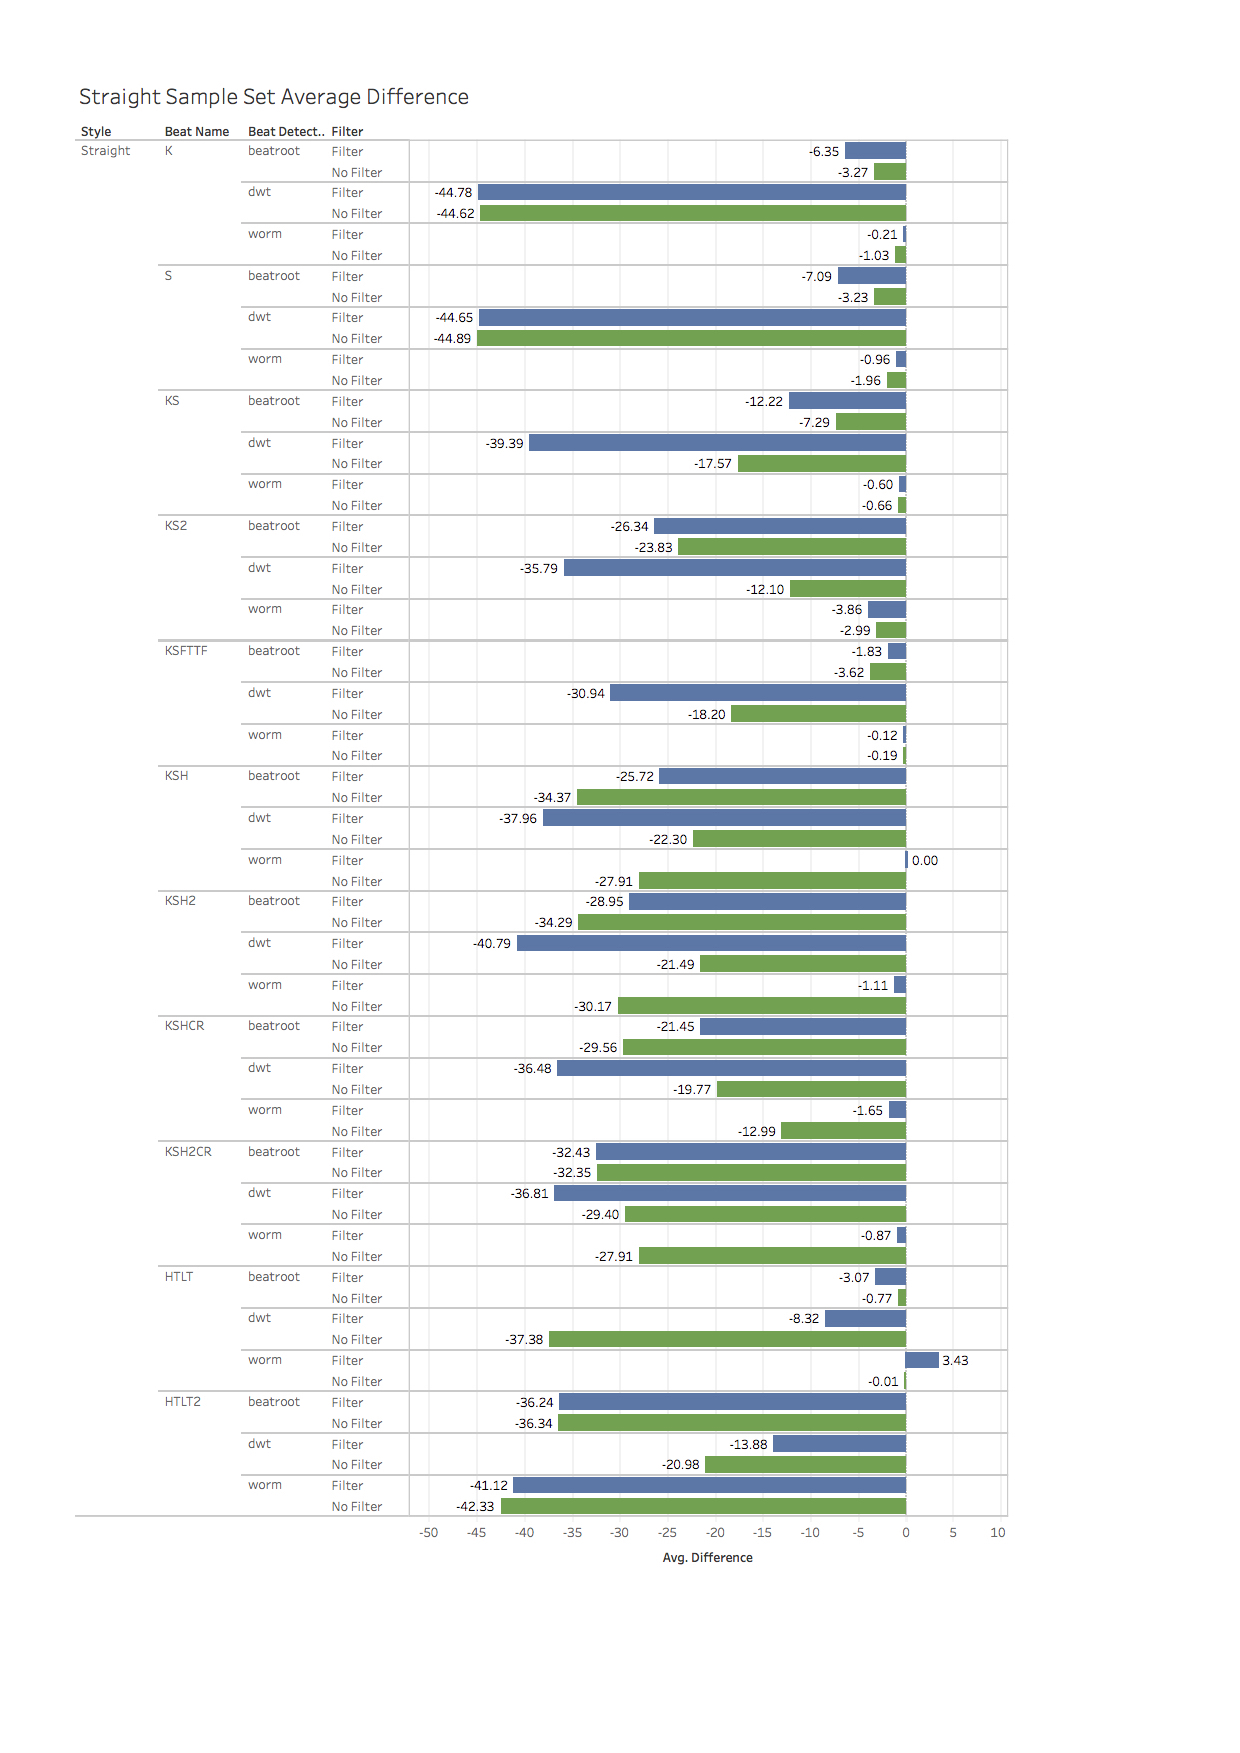
\includegraphics[scale=0.38]{images/SSSAD.jpg}
\caption{Straight sample set average difference results}
\label{fig: stradAveDiff}
\end{figure}

When the corrected difference values are applied to the data set the accuracy of the Tzanetakis \textit{et al}'s \cite{tzane1} DWT method increases significantly (Figure~\ref{fig: stradAveDiffCor}). Although, it does return its least accurate results for the samples consisting of a crash cymbal and the high and low tom-toms. The affect of the crash cymbal on the accuracy of the tempo recorded confirms the suspicion that loud cymbals will adversely affect the accuracy of the beat detection algorithms. The low accuracy recorded by the DWT method for the HTLT2 sample set where the time element is played on the low tom-tom. Suggesting, the possibility that this method will not respond as well when there are not distinct frequencies playing each part of the drum beat. \par

\begin{figure}[htbp]
\centering
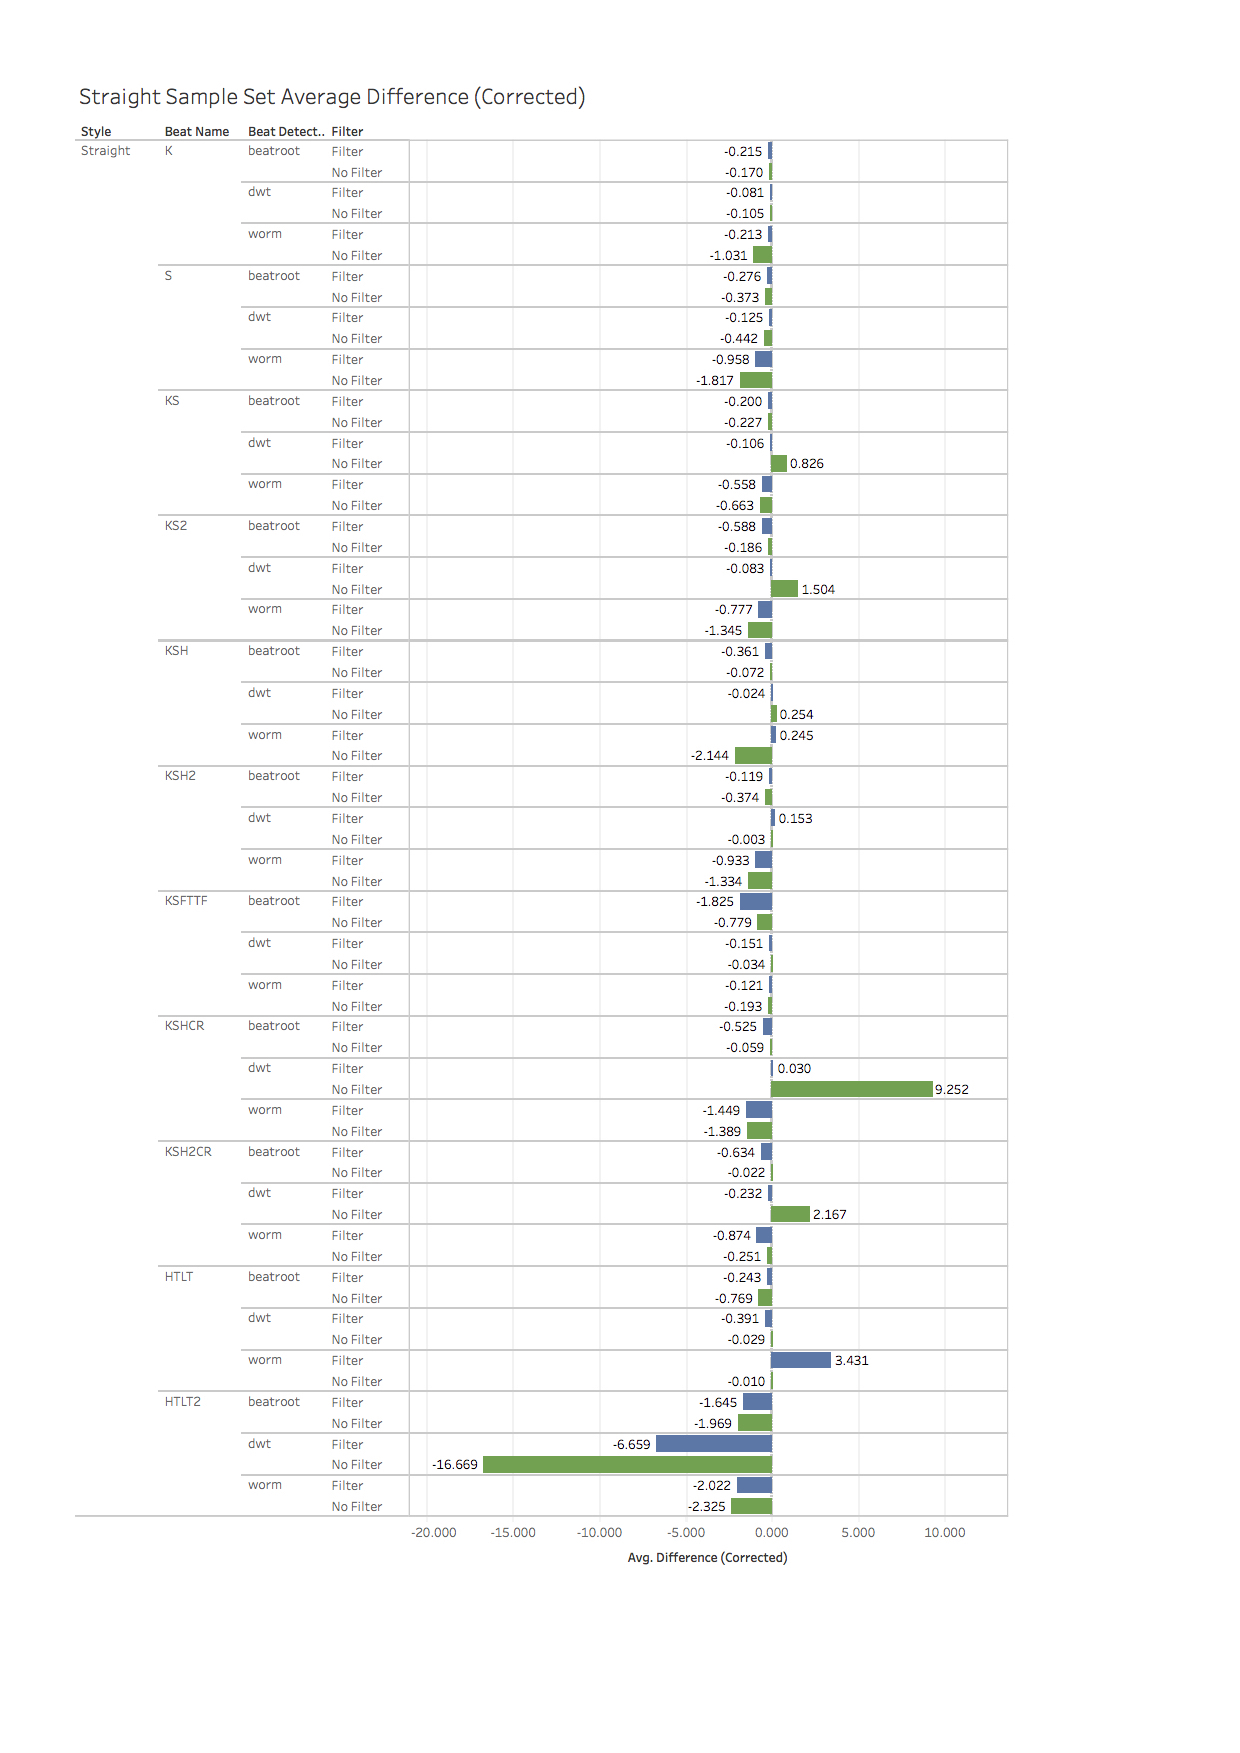
\includegraphics[scale=0.38]{images/SSSADC.jpg}
\caption{Straight sample set average difference results with correction applied}
\label{fig: stradAveDiffCor}
\end{figure}

Also, within this data set the results produced for the single drum samples can be observed to actually have some of lowest levels of accuracy. This is improved once the corrected values are introduced, suggesting that the issue of doubling was particularly prevalent for these samples. 

\subsection{Swing Sample Results}
The doubling of calculated tempos was not as prevalent within the Swing sample set. Both the original (Figure~\ref{fig: swingAveDiff}) and the corrected (Figure~\ref{fig: swingAveDiffCor}) difference values were significantly high. Although, the Tzanetakis \textit{et al}'s \cite{tzane1} DWT method's accuracy is again improved by the updated difference values, the Beatroot and PW's performance remains very similar across both data sets.

\begin{figure}[htbp]
\centering
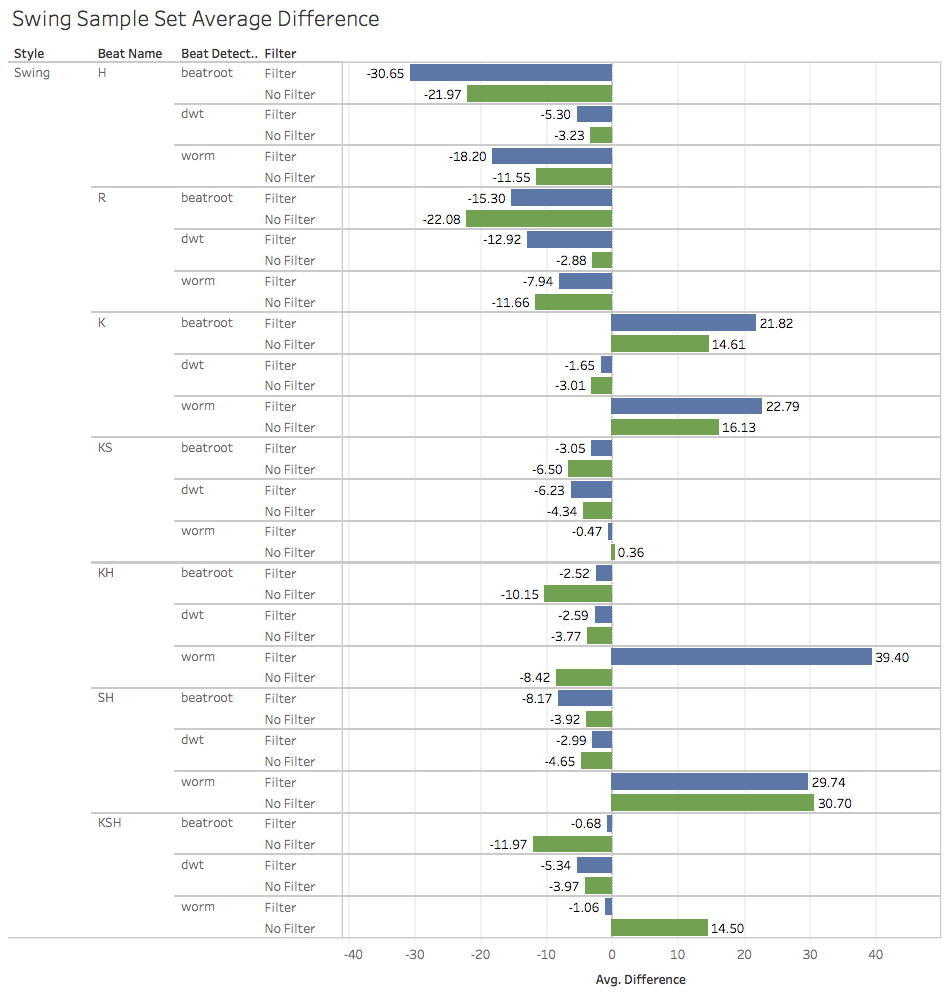
\includegraphics[scale=0.45]{images/SwiSSAD.jpg}
\caption{Swing average difference results}
\label{fig: swingAveDiff}
\end{figure}

\begin{figure}[htbp]
\centering
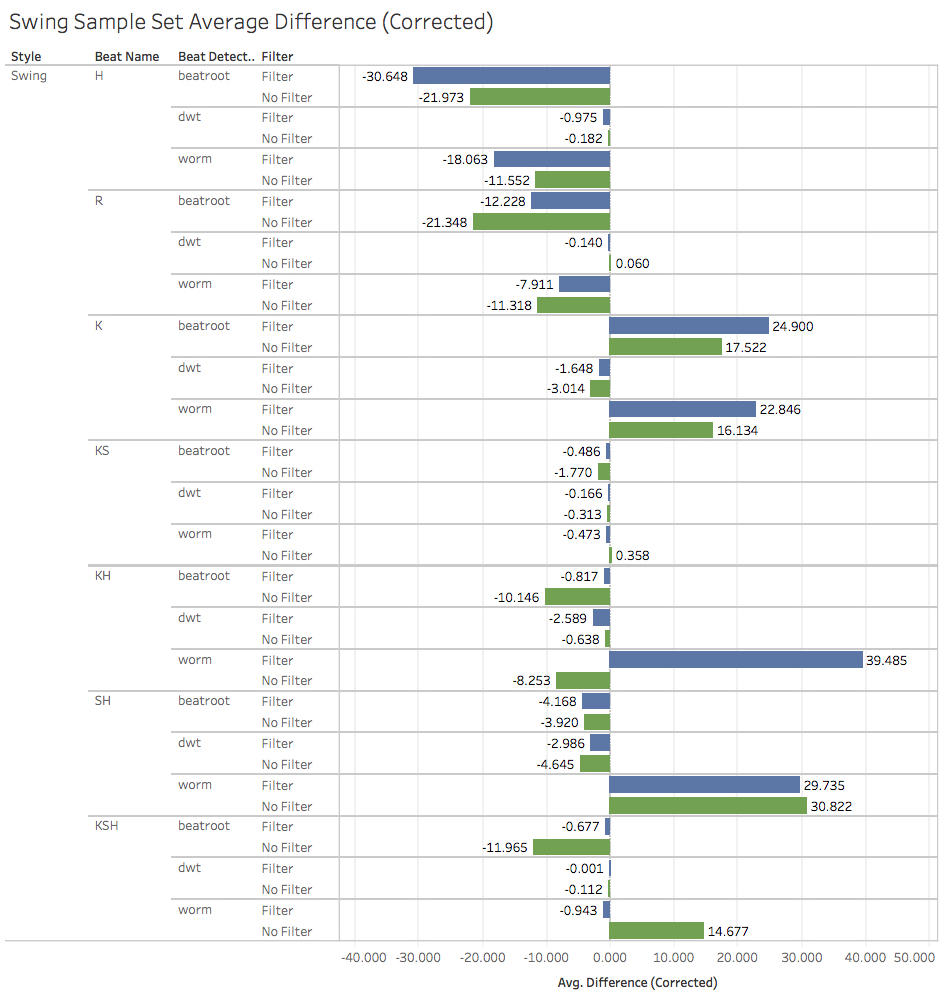
\includegraphics[scale=0.45]{images/SwiSSADC.jpg}
\caption{Swing average difference results with correction applied}
\label{fig: swingAveDiffCor}
\end{figure}

The single drum elements within this data set were expected to cause some problems, due to their use of triplets. This can be seen for both the R and H sample sets within Figure~\ref{fig: swingAveDiff}. Once the corrected values are applied the DWT method does return a higher level of accuracy. However, the accuracy of both Beatroot and the PW are relatively unaffected by the introduction of the corrected values.

\subsection{Off-Beat Sample Results}

The last group of style results utilise a time element being played on the off-beat. The rest of the beat is considered to be straight. It is to be expected then that the results exhibit a similar amount of potential doubling of the tempo values as with the straight data set (Figure~\ref{fig: offAveDiff}).

\begin{figure}[htbp]
\centering
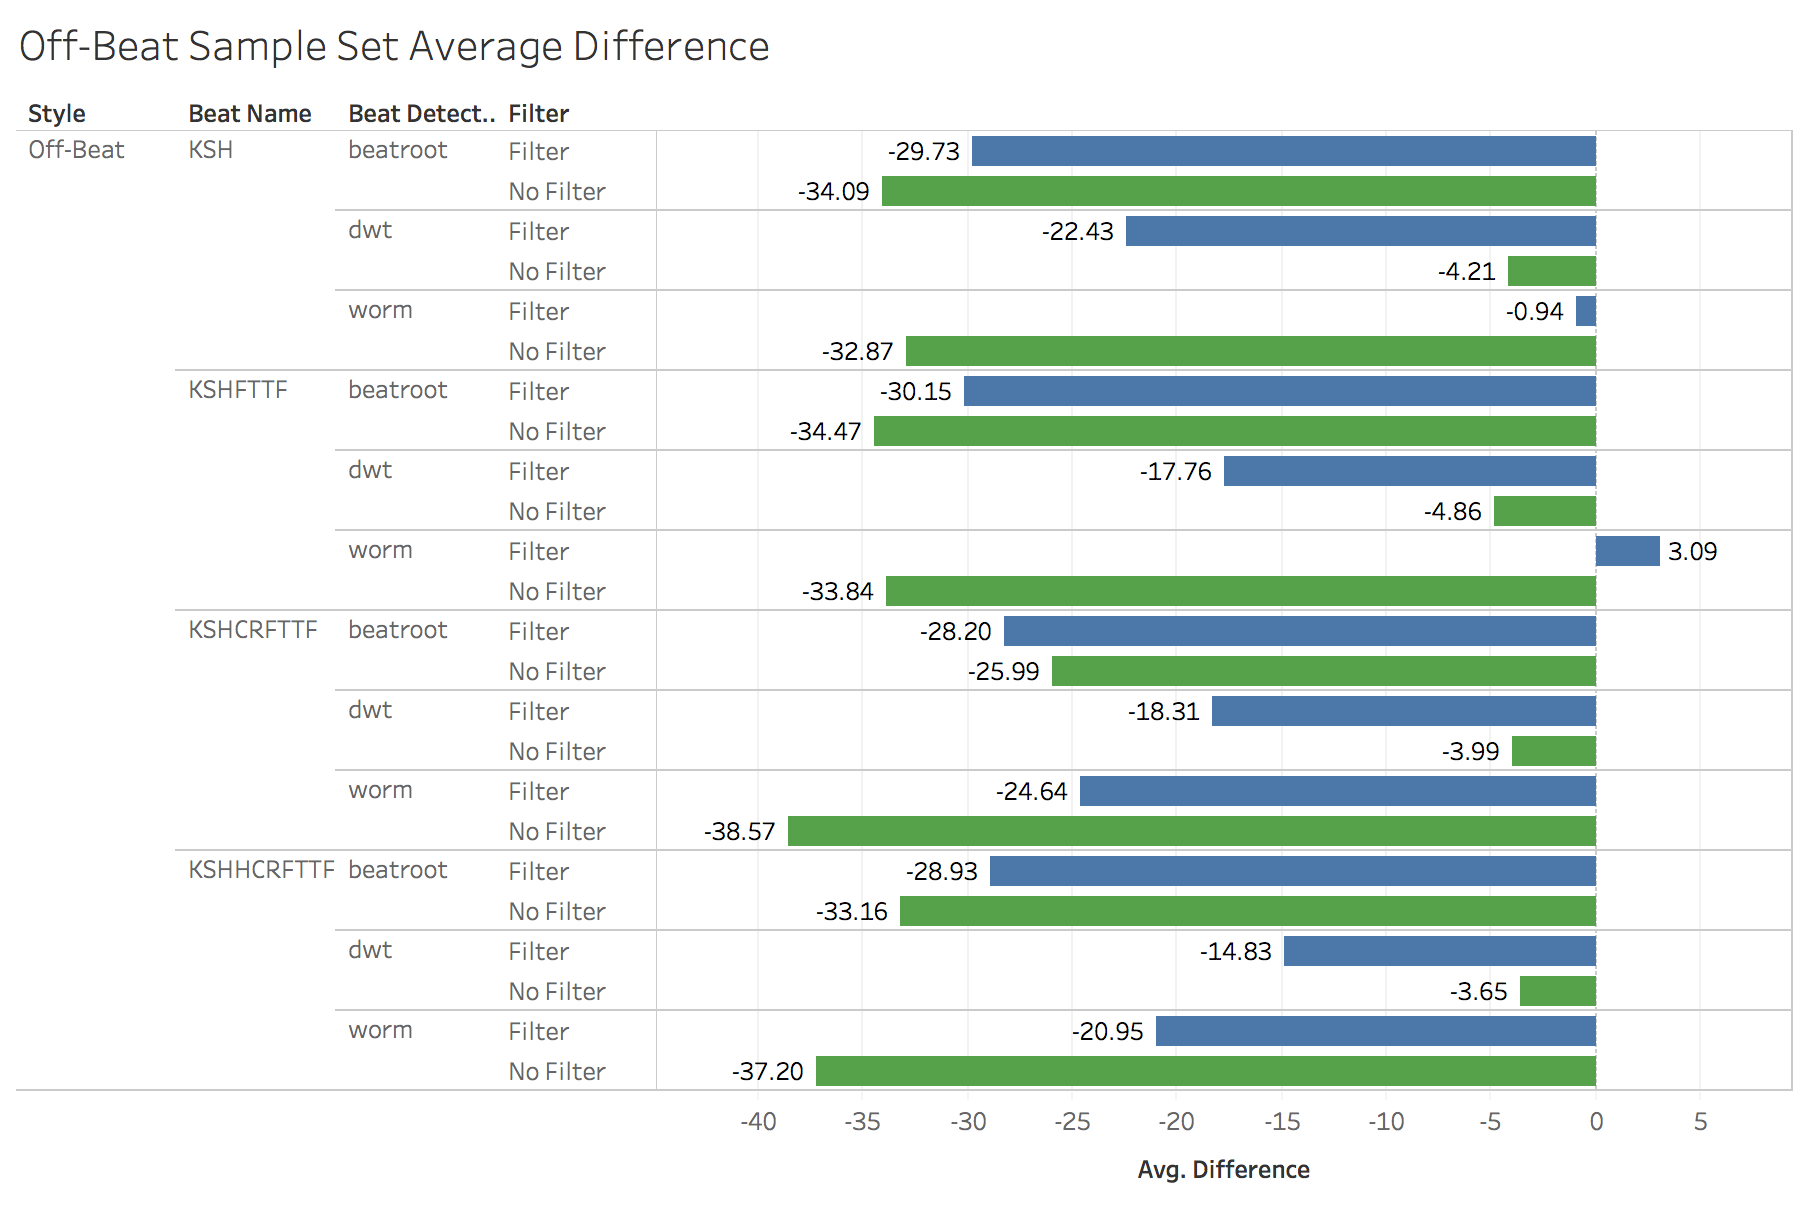
\includegraphics[scale=0.25]{images/OBSSAD.jpg}
\caption{Off-Beat average difference results}
\label{fig: offAveDiff}
\end{figure}

When the corrected difference values are introduced the accuracy is again improved (Figure~\ref{fig: offAveDiffCor}). For the louder KSHHCRFTTF sample, the Beatroot and PW both recorded a lower level of accuracy with the low-pass filter than without. It is expected that the low-pass filter would help to remove some of the noise produced by the cymbals in this sample. However, this result suggests that by removing the higher frequencies produced by cymbals can adversely affect the accuracy of these two tempo calculation methods.

\begin{figure}[htbp]
\centering
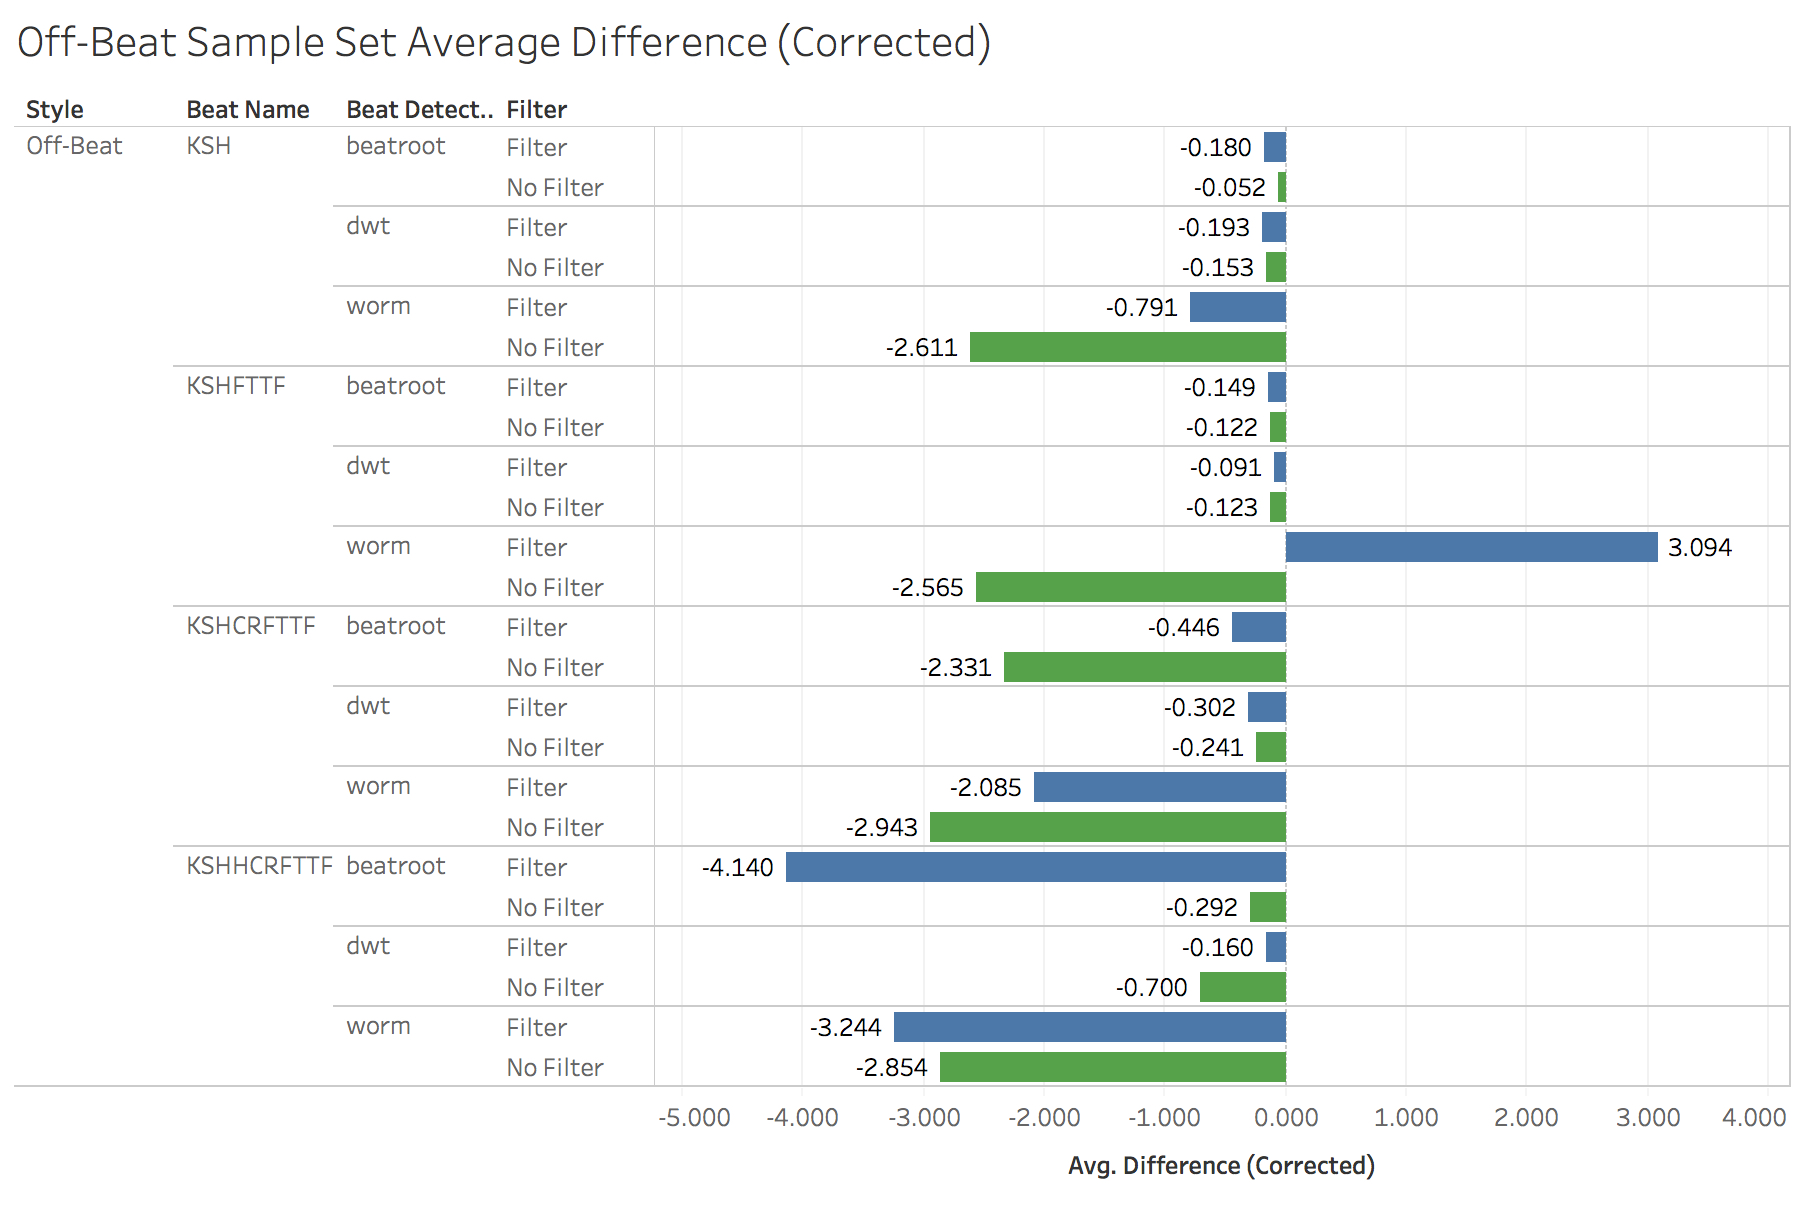
\includegraphics[scale=.25]{images/OBSSADC.jpg}
\caption{Off-Beat average difference results with correction applied}
\label{fig: offAveDiffCor}
\end{figure}

\subsection{Low Tempo Comparison}
During the testing process it was noted that the result doubling seemed to be prominent for samples being played at lower tempos. Usually anything with a bpm of one hundred and below. To investigate if the algorithms performed better with higher tempos regardless of style, a doubling count was applied to the data set. Using the same error margin applied previously. 

\begin{sidewaysfigure}[htbp]
\centering
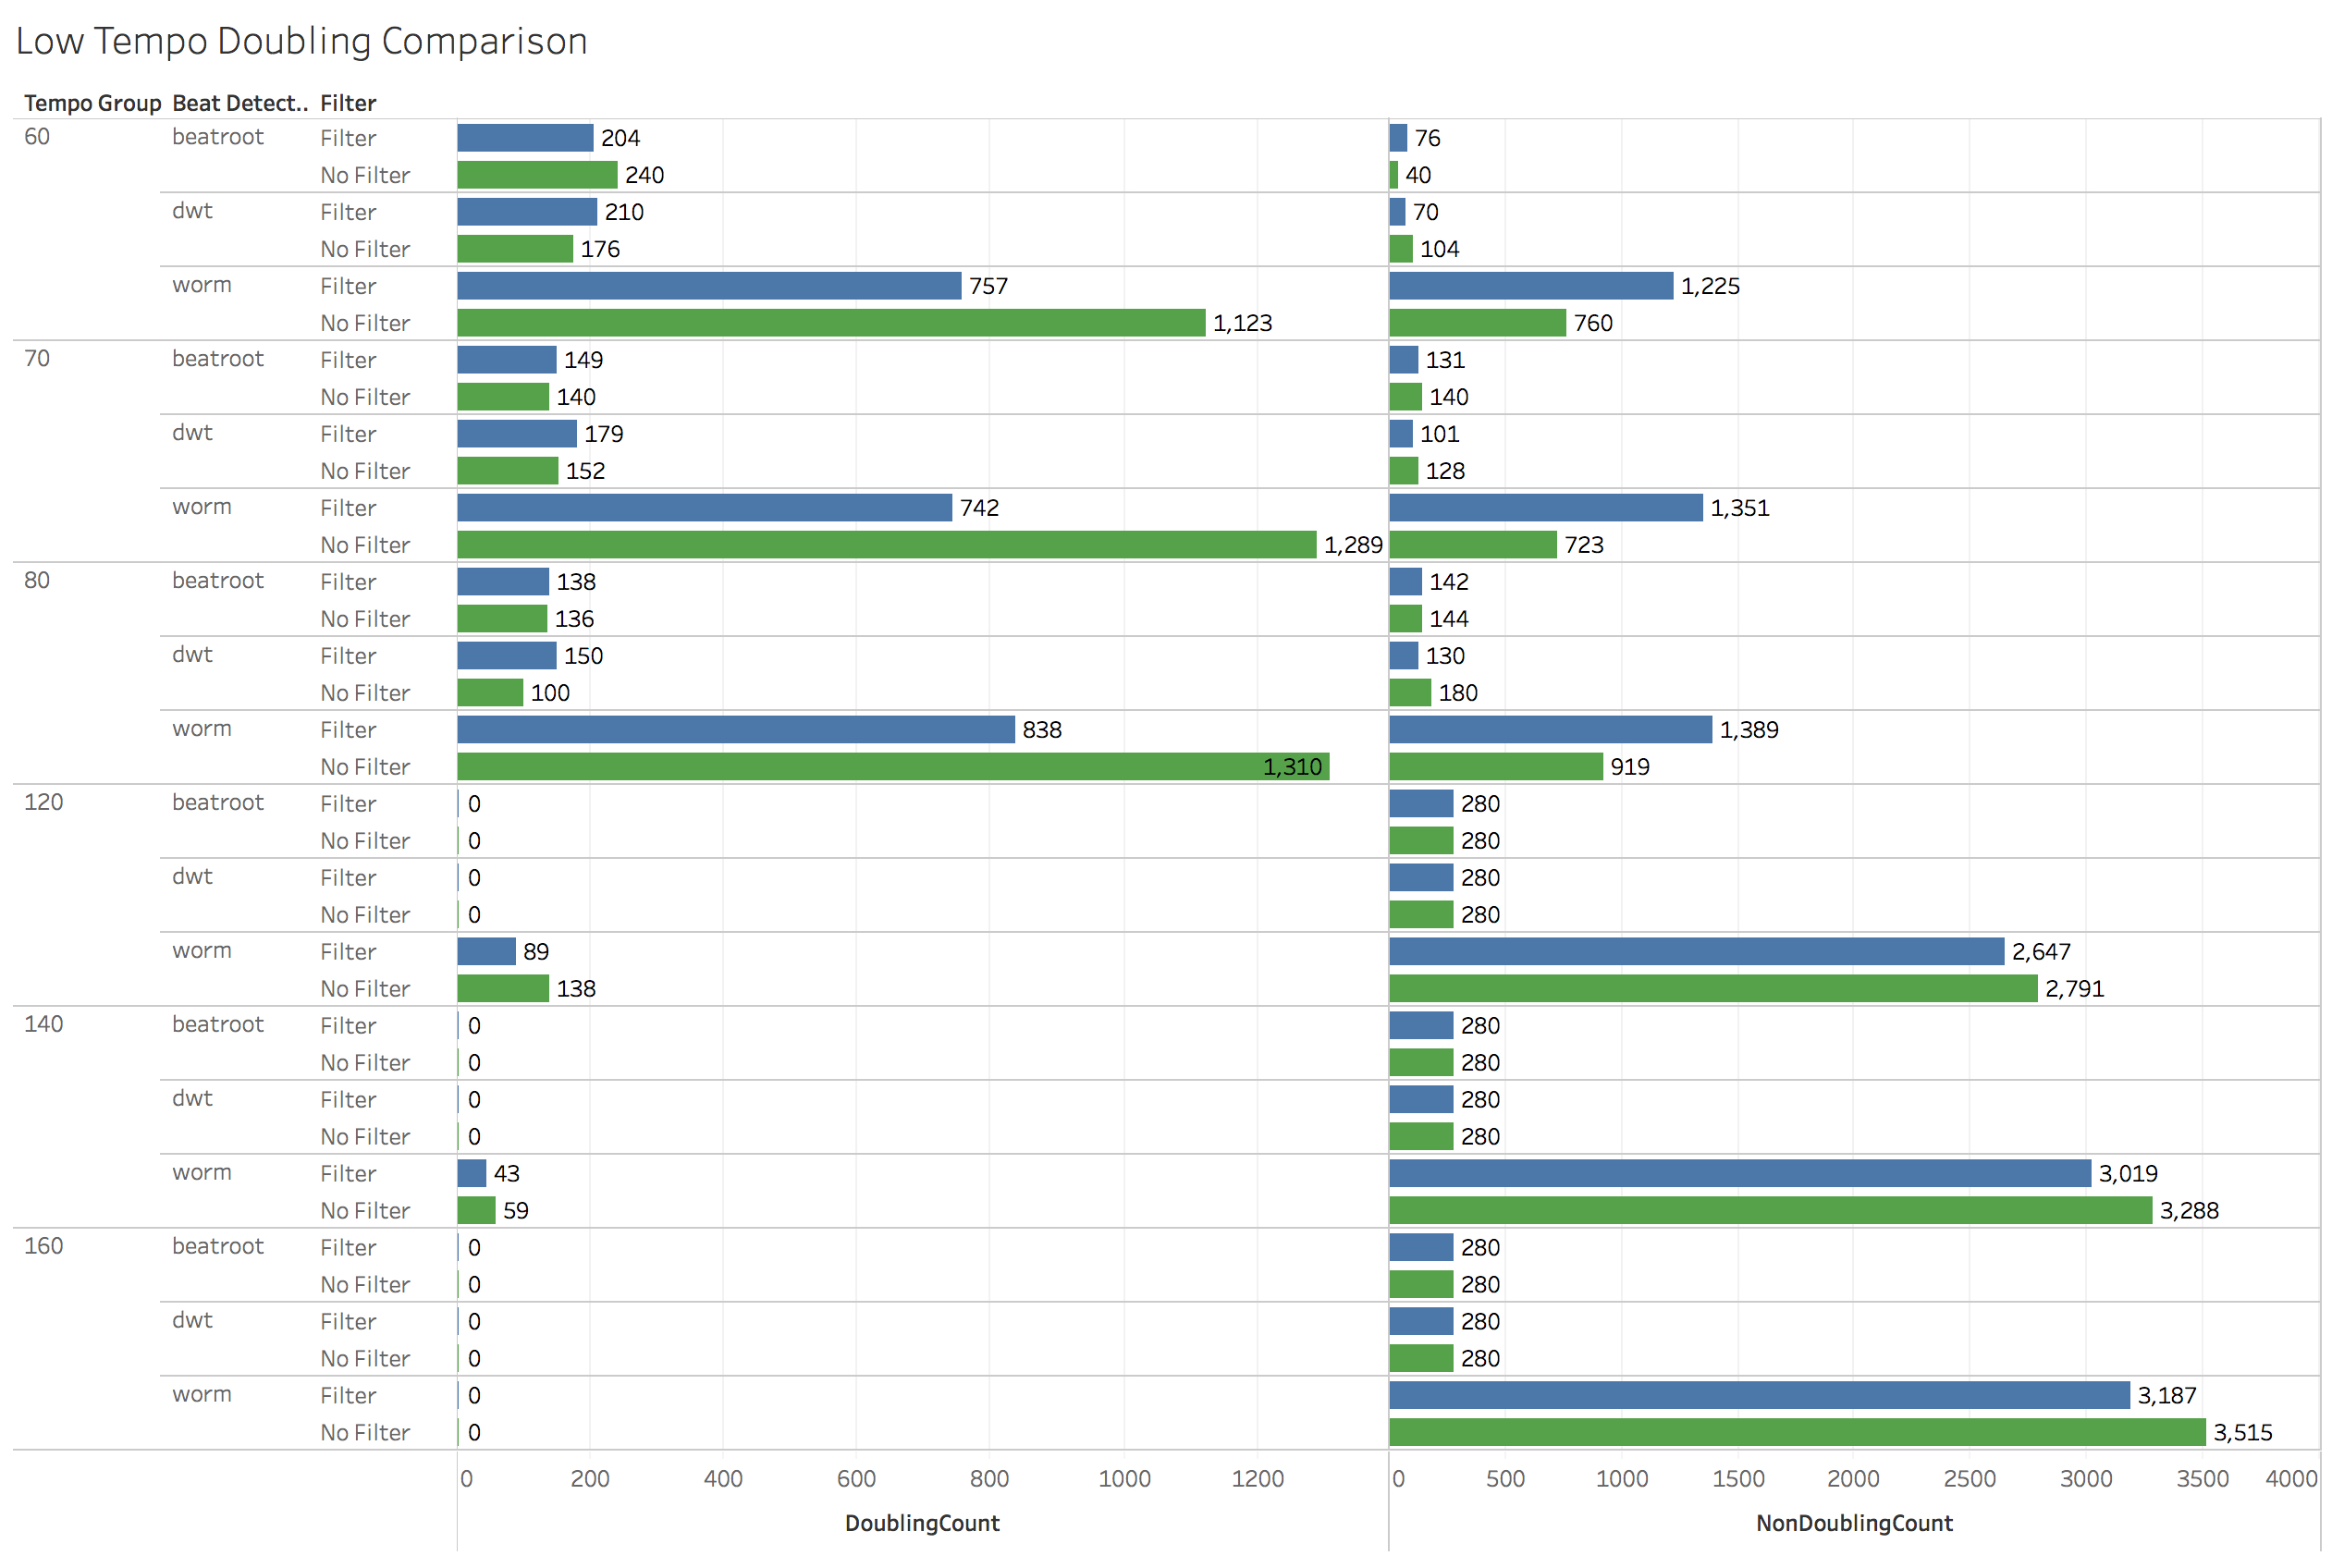
\includegraphics[scale=0.25]{images/LowDoubling.jpg}
\caption{Low tempo comparison}
\label{fig: lowTemCom}
\end{sidewaysfigure}

The results viewed in Figure~\ref{fig: lowTemCom}, confirm that the all three of the beat detection algorithms produce significantly less doubling when processing drum beats with higher tempos. If the style grouping is introduced (see Figure~\ref{fig: lowTemComStyle}, it is apparent that the doubling is most prevalent with the straight sample set. Out of the three algorithms, the PW returns the highest count of doubled results. Although, this is to be expected as the PW returns a larger number of tempo values per sample.

\begin{sidewaysfigure}[htbp]
\centering
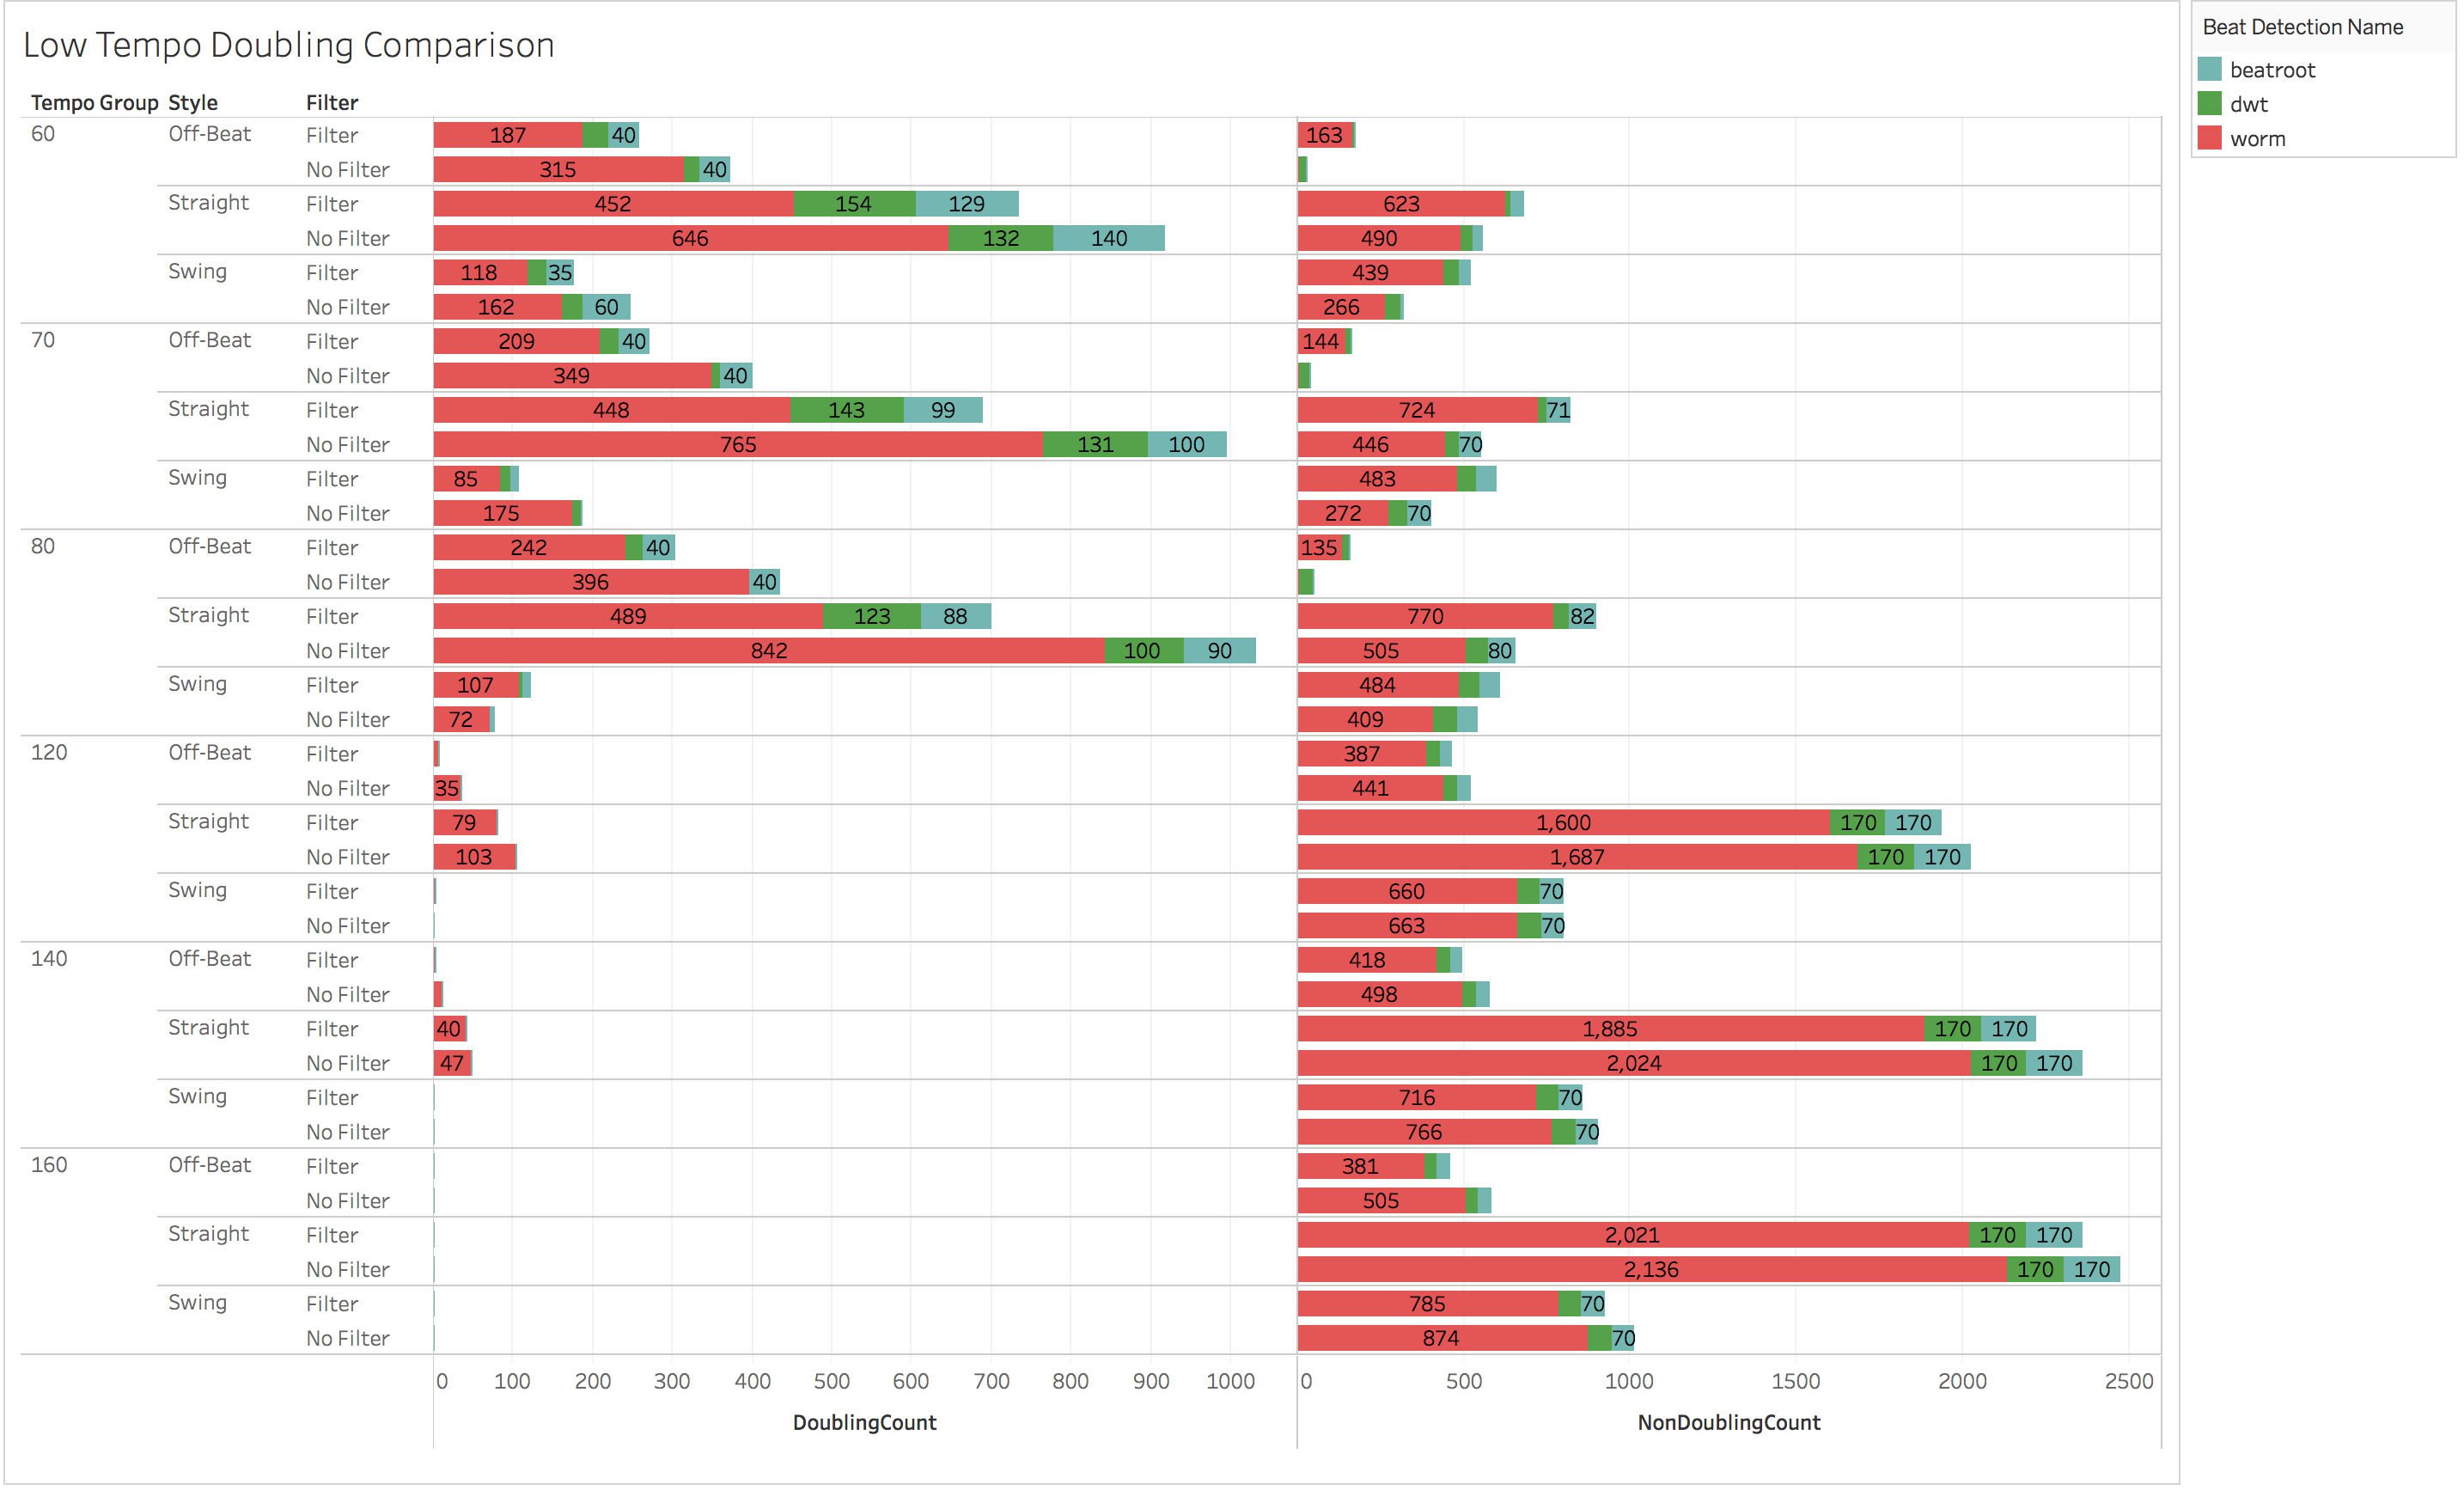
\includegraphics[scale=0.25]{images/lowStyle.jpg}
\caption{Low tempo comparison with style groupings}
\label{fig: lowTemComStyle}
\end{sidewaysfigure}

\subsection{Beat Detection Response Time}
Due to the smaller window size utilised by the PW it is expected to perform the best within this comparison. The response time was recorded by the RTT\_Analyser when the first returned tempo was plus or minus one bpm from the expected tempo result. 

Before this could be calculated the all of the tempo results produced by the PW for expected tempos of seventy five were removed. As the PW's first result returned regardless of expected tempo was always seventy five. Despite this and as expected the PW returned the fastest tempo value (see Figure~\ref{fig: resTime}). Returning a tempo within the margin of error for the straight KSH2 beat within 0.675 seconds when processing through the low-pass filter. Then without a filter a tempo was produced in 0.660 seconds. 

\begin{figure}
\centering
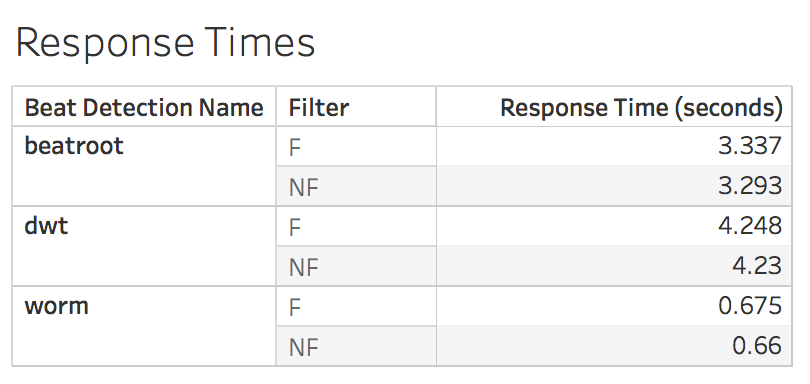
\includegraphics[scale=0.3]{images/ResponseTime.jpg}
\caption{Fastest response times recorded by the RTT\_Analyser}
\label{fig: resTime}
\end{figure}

\subsection{Overall Tempo Accuracy}
The overall tempo accuracy was calculated by counting the number of tempo results that were plus or minus one bpm away from the expected tempo. The results for the three beat detection methods with and without a filter were then compared. A corrected value was also included to show the possible level of accuracy if the issue of doubling was not present (Figure~\ref{fig: OTA}).

\begin{figure}[htbp]
\centering
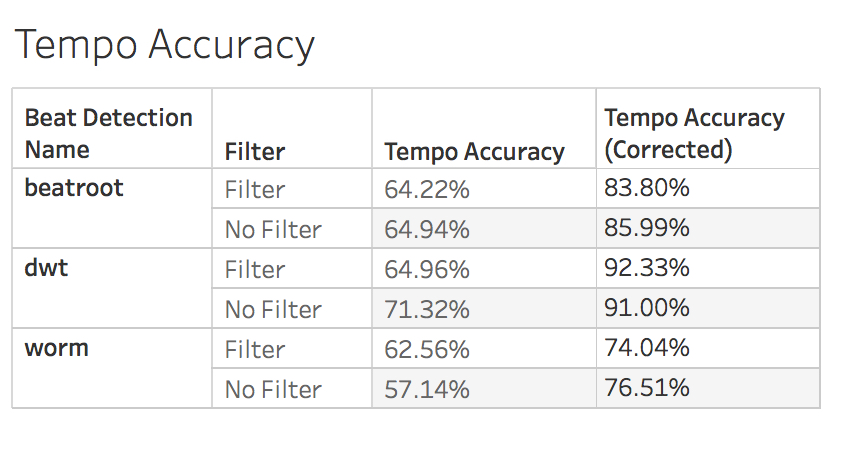
\includegraphics[scale=0.35]{images/TempoAcc.jpg}
\caption{Overall tempo accuracy}
\label{fig: OTA}
\end{figure}

Unsurprisingly, the Tzanetakis \textit{et al}'s \cite{tzane1} DWT method performed with the highest level of accuracy. Interestingly, without the corrected values all three systems produced a consistent level of accuracy when using the low-pass filter. Without the filter though, the DWT method produced the highest overall accuracy of 71.32\% and the PW produced the least of 57.12\%.\par

The corrected results show that there is a clear distinction between the accuracy of the three methods. With the DWT method exhibiting the most potential followed by the Beatroot system and then the PW. The effectiveness of the low-pass filter is hard to ascertain from these results alone. However, based on the five percent increase to the overall tempo accuracy, it can be said that the PW benefited the most from the inclusion of the filter.

\subsection{Filter/Non-Filter Comparison}
To ascertain the effectiveness of the low-pass filter applied to the RTT\_Analyser, the number of uncorrected tempo records within one bpm were collated for the sample sets with and without a filter. The number of records that fell within this accuracy margin and the percentage of the total number of tempo records can be seen in Figure~\ref{fig: allFilAcc}. 

\begin{figure}[htbp]
\centering
\vspace{-1in}
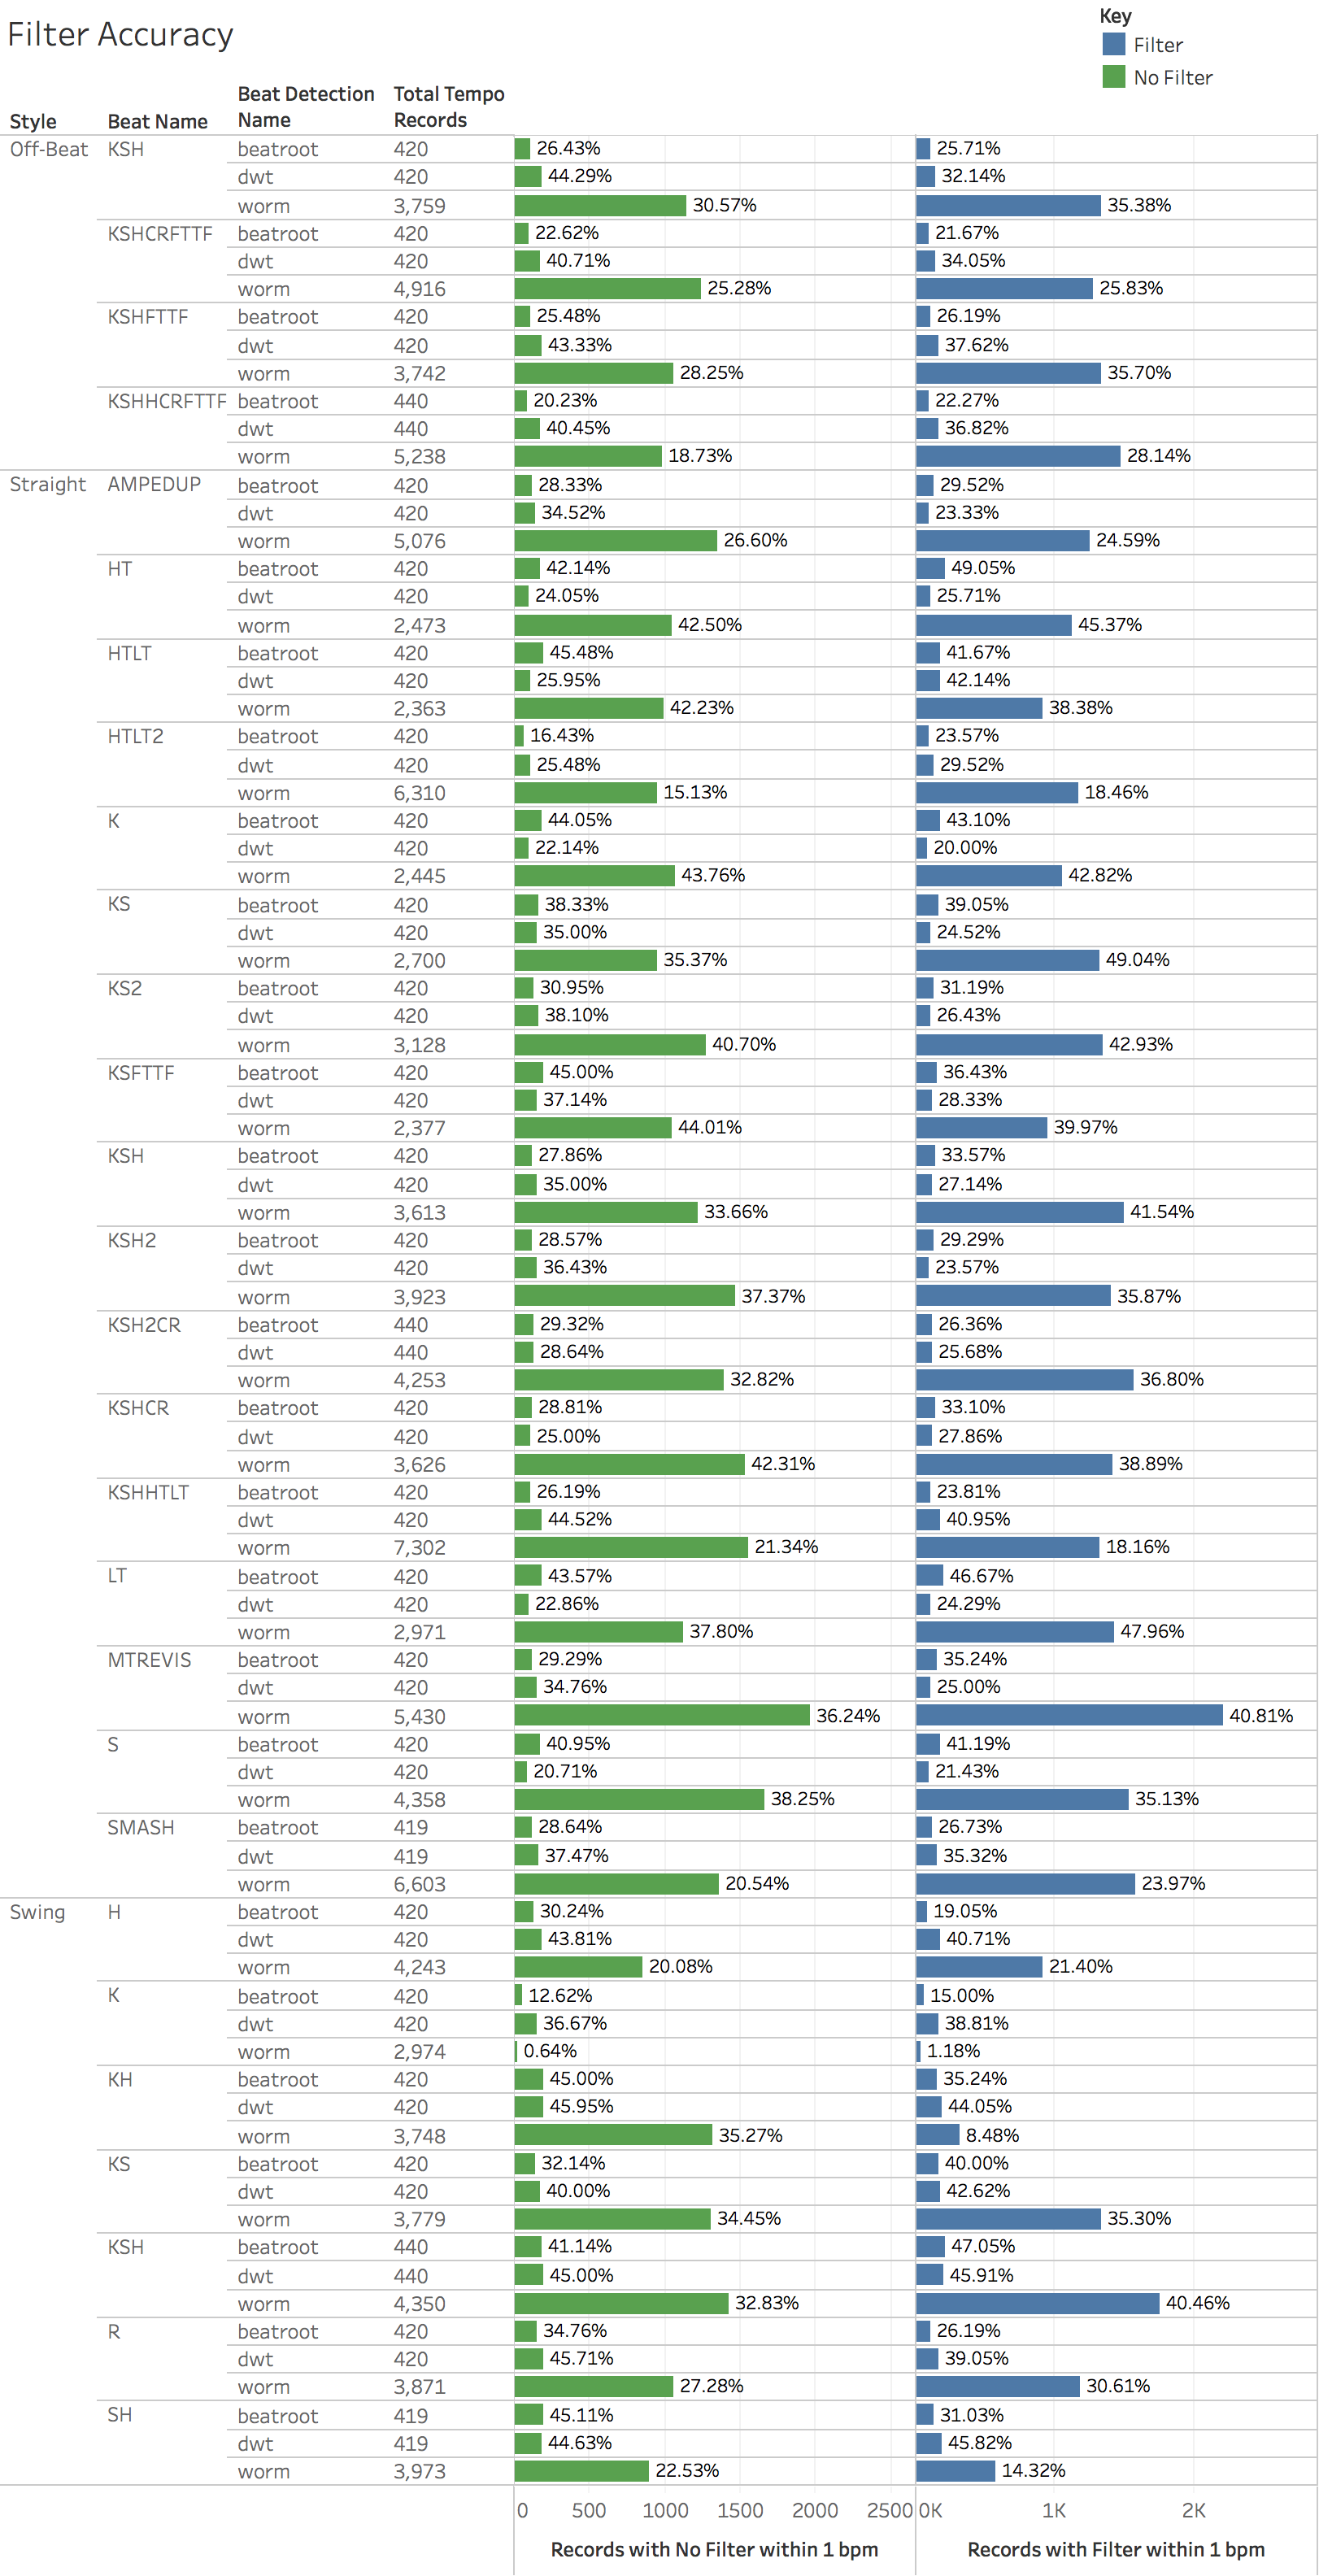
\includegraphics[scale=0.3]{images/filterAcc.png}
\caption{Filter/No Filter Accuracy Comparison, split by style and sample set}
\label{fig: allFilAcc}
\end{figure}

The results show a slightly higher level of accuracy is provided for the sample set which used a low-pass filter but it is very marginal. The overall comparison of the total number of records can be seen in Figure~\ref{fig: overFilAcc}, which further highlights the slight increase in accuracy offered by the introduction of a low-pass filter. 

\begin{figure}[htbp]
\centering
\vspace{-1in}
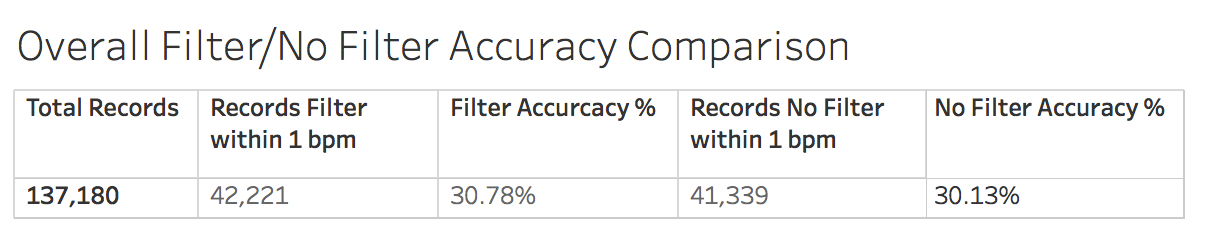
\includegraphics[scale=0.3]{images/OverFilAc.jpg}
\caption{Filter/No Filter Accuracy Comparison of total records}
\label{fig: overFilAcc}
\end{figure}

\clearpage
\maketitle \section{Evaluation and Discussion}

\subsection{Project Successes}

A key success of the project was during the live audio testing phase of the project, where the RTT\_Analyser processed just under ten hours of audio without an issue, producing well over 130,000 different tempo records.

By collecting a large data set, it was possible to confidently assess whether any of the three beat detection algorithms were suitable to be implemented as part of a training tool for drummers. From the data set, it is clear that the Tzanetakis \textit{et al}'s \cite{tzane1} DWT method offers the highest level of accuracy, with the potential of even higher if the issue of doubling is resolved. However, the response time of the Tzanetakis \textit{et al}'s \cite{tzane1} DWT method might be an issue. \par 

Another success was the actor system used in the RTT\_Analyser. The development of this system was straightforward and intuitive, it provided a reliable parallel processing and no failures were recorded during the beat detection testing process. 

\subsection{Project Challenges}

One challenge experienced during the development of the RTT\_Analyser, was that the adaption of the Beatroot system to work with live audio took longer than anticipated. This was mainly due to the difficulty of working with a large pre-existing code base. To overcome this, the mitigation protocol set out in the project proposal was followed and an alternative system was sourced; the Performance Worm. This ensured that the project did not fall any further behind schedule.\par 

The delay in development caused by this issue, led to insufficient time for the author to implement the Tzanetakis \textit{et al}'s \cite{tzane1} beat detection algorithm. Although, there was a mitigation protocol in place, there was insufficent time to implement this, so a different course of action was chosen. A preexisting Scala implementation of the Tzanetakis \textit{et al}'s \cite{tzane1} DWT method by Marco Ziccard\cite{marcoZin} was used. Using this implementation, allowed for the regaining of the time lost during the initial failed attempt to adapt the Beatroot system. This ensured the project not only remained on schedule, but there was also sufficient time to try adapting the Beatroot system again. This was completed successfully on the second attempt.\par

One unforeseen challenge was presented by the original decision to use JSON files for data storage. Due to the inclusion of the PW beat detection algorithm in the RTT\_Analyser and the decision to run tests with a low-pass filter and without, the number of records recorded by the RTT\_Analyser increased significantly. The original estimate was for approximately 700 files each holding approximately ten results per beat detection method. The final number of results collection was 130,000 plus. JSON is more than adequate for holding this much data, an issue arose when the data visualisation software package, Tableau\cite{tableau} was used. As Tableau does not work with JSON files, the data would need to be converted to another format. Due to limited time the data was converted to an Excel\cite{excel} file. This required a large amount of data manipulation to be carried out. A number of Visual Basic for Applications (VBA) macros were written to perform the data manipulation, and once the data was in the required format it was connected to Tableau where any further manipulation and analysis of the data could be performed much more efficiently. 


\subsection{Future Work}
There are a number of possible routes to consider with regard to the future development of the RTT\_Analyser, including, further investigations into the doubling issue, user interface improvements, adaption of the data storage method, and converting the RTT\_Analyser into a mobile training tool application.\par

A key improvement to the RTT\_Analyser would be to alleviate the doubling issue presented during this project. To do this, a function to log the frequencies detected by the beat detection algorithms during live audio capture could be added to the RTT\_Analyser. This could be achieved by logging the data produced by the parts of the Beatroot and Tzanetakis \textit{et al}'s \cite{tzane1} DWT method that perform the original signal processing. This data can be examined to see if any particular frequencies are the cause of this issue.\par

Alternatively, the analysis could be performed on the drum beat samples before they are processed by the RTT\_Analyser. The goal of this analysis would be to produce a frequency map of the samples. This data could then be compared with the output of the RTT\_Analyser in an attempt to discover if there are particular frequencies for which doubling occurs.\par

The user interface utilised by the RTT\_Analyser is intended to be basic, however, if a some new features were added to it it could provide an improved user expereince. One such feature could be a visualisation of the audio as it is being captured, which could assist the frequency map function in determining the cause of the doubling issue.

If further drum beat testing is to be carried out, then adapting the data storage method of the RTT\_Analyser from JSON files to a relational database should be considered. One option is to set up a MongoDB\cite{mongo} database to hold the RTT\_Analyser's data. An advantage of this is that the data structure used by MongoDB is very similar to structure of JSON objects. This would enable the existing data structures used by the RTT\_Analyser to be maintained. Alternatively, the RTT\_Analyser could be adapted to work with an SQL database, which could be the easier option, due to the author's familiarity with SQL.\par  

Although, the accuracy of the beat detection algorithms used in the RTT\_Analyser is not on the same level as the midi training tools, they could still provide a useful tool for a drummer. One possible route would be to develop an application for mobile devices which combines a metronome with the RTT\_Analyser. A drummer could then use this application to aid their practice session by using the metronome to set the tempo. After a predetermined amount of time the metronome would stop and the drummer continues to play. While doing so, the application would report as to whether they have remained at the same tempo as the metronome or if their tempo has fluctuated. Such a tool would definitely provide a useful training aid to any drummer wanting to work on their timing.







\newpage
\begin{thebibliography}{99}
\bibitem{midi}
\textit{http://www.instructables.com/id/What-is-MIDI/}
\bibitem{oxford-comp}
Alison Latham\\
\textit{The Oxford Companion to Music, 2002, Oxford University Press}
\bibitem{brit-metro} 
\textit{https://www.britannica.com/art/metronome}
\bibitem{drum-bible}
Mick Berry and Jason Gianni\\
\textit{The Drummer's Bible: How to Play Every Drum Style from Afro-Cuban to Zydeco, Second Edition, 2004, See Sharp Press}
\bibitem{drum-note}
\textit{http://www.drummagazine.com/lessons/post/drumkey/}
\bibitem{allen-danneburg}
Paul E. Allen and Roger B. Dannenberg\\
\textit{Tracking Musical Beats in Real Time, International Computer Music Conference, International Computer Music Association, 1990, pp. 140-143}
\bibitem{longeut1}
H. C Longuet-Higgins\\
\textit{Perception of melodies, Nature Vol. 263, 1976, pp. 646-653}
\bibitem{dixon1}
Simon Dixon\\
\textit{Automatic Extraction of Tempo and Beat from Expressive Performances. Journal of New Music Research, 30 (1), 2001, pp 39-58}
\bibitem{dixon2}
Simon Dixon\\
\textit{Onset Detection Revisited, Proceedings of the 9th International Conference on Digital Audio Effects, Montreal, September 2006, pp 133-137}
\bibitem{dixon3}
Simon Dixon\\
\textit{On the Analysis of Musical Expression in Audio Signals. Storage and Retrieval for Media Databases, SPIE-IS\&T Electronic Imaging, SPIE Vol. 5021, 2003 pp 122-132}
\bibitem{mirex-onset}
\textit{http://www.music-ir.org/mirex/wiki/2016:Audio\_Onset\_Detection}
\bibitem{sonic}
\textit{http://www.ieor.berkeley.edu/~ieor170/sp15/files/Intro-to\_Sonic\_Events\_Campion.pdf}
\bibitem{onset-tut}
Juan Pablo Bello, Laurent Daudet, Samer Abdallah, Chris Duxbury, Mike Davies, and Mark B. Sandler 
\textit{A Tutorial on Onset Detection in Music Signals, IEEE TRANSACTIONS ON SPEECH AND AUDIO PROCESSING, VOL. 13, NO. 5, 2005, pp. 1035 - 1047}
\bibitem{mirex-main}
\textit{http://www.music-ir.org/mirex/wiki/2005:Main\_Page}
\bibitem{tzane1}
George Tzanetakis, Georg Essl and Perry Cook\\
\textit{Audio Analysis using the Discrete Wavelet Transform, Proc. WSES International Conference on Acoustics and Music: Theory and Applications (AMTA), 2001}
\bibitem{mirex-06}
\textit{http://www.music-ir.org/mirex/wiki/2006:Audio\_Beat\_Tracking\_Results}
\bibitem{dixon4}
Simon Dixon\\
\textit{Evaluation of the Audio Beat Tracking System BeatRoot. Journal of New Music Research, 36, 1, 2007, pp 39-50}
\bibitem{polikapt2}
\textit{http://users.rowan.edu/ polikar/WAVELETS/WTpart2.html}
\bibitem{lyons}
Richard G. Lyons\\
\textit{Understanding Digital Signal Processing, Third Edition, Prentice Hall, 2010}
\bibitem{tzane2}
Tao Li, Mitsunori Ogihara, George Tzanetakis\\
\textit{Music Data Mining, CRC Press, 2002, pp 45-53}
\bibitem{tzane3}
George Tzanetakis and Perry Cook\\
\textit{Musical Genre Classification of Audio Signals, IEEE TRANSACTIONS ON SPEECH AND AUDIO PROCESSING, VOL. 10, NO. 5, JULY 2002}
\bibitem{smith}
Steven W. Smith\\
\textit{The Scientist and Engineer's Guide to Digital Signal Processing, California Technical Publishing, 2011, Chapter 3}
\bibitem{pallas}
Ramón Pallás-Areny and John G. Webster\\
\textit{Analog Signal Processing, Wiley, 199, pp. 231}
\bibitem{dixonGoeblWidmer}
Simon Dixon, Werner Goebl and Gerhard Widmer\\
\textit{The Performance Worm: Real Time Visualisation of Expression based on Langner’s Tempo-Loudness Animation, International Computer Music Conference, 16 - 21 September 2002, Göteborg, Sweden, pp 361-364.}
\bibitem{pulseWag}
Bill Waggener\\
\textit{Pulse Code Modulation Techniques}
\bibitem{soundTrail}
Oracle\\
\textit{https://docs.oracle.com/javase/tutorial/sound/}
\bibitem{akkaActors}
Akka\\
\textit{http://doc.akka.io/docs/akka/2.4.9/scala/actors.html}
\bibitem{reactMan}
Jonas Bonér, Dave Farley, Roland Kuhn, and Martin Thompson\\
\textit{Reactive Manifesto, http://www.reactivemanifesto.org/}
\bibitem{acotrsys}
Akka\\
\textit{http://doc.akka.io/docs/akka/2.4.9/general/actor-systems.html}
\bibitem{sbt}
Josh Suereth and Matthew Farwell\\
\textit{SBT in Action: The simple Scala build tool, Manning Publications, 2015}
\bibitem{javasound}
Oracle\\
\textit{https://docs.oracle.com/javase/8/docs/technotes/guides/sound/programmer\_guide/contents.html}
\bibitem{desouze}
\textit{https://github.com/ederwander/Beat-Track}
\bibitem{marcoZin}
\textit{https://github.com/mziccard/scala-audio-file}
\bibitem{green}
Andrew Greensted
\textit{http://www.labbookpages.co.uk/audio/javaWavFiles.html}
\bibitem{mariusEr}
Marius Eriksen\\
\textit{Effective Scala, http://twitter.github.io/effectivescala/}
\bibitem{odesky}
Martin Odersky, Lex Spoon and Bill Venners\\
\textit{Programming in Scala, Second Edition, Artima Press, 2010}
\bibitem{play}
\textit{https://www.playframework.com/documentation/2.5.x/ScalaJson}
\bibitem{json}
\textit{http://www.json.org/}
\bibitem{play-writes}
\textit{https://www.playframework.com/documentation/2.5.x/api/scala/index.html\#play.api.libs.json.Writes}
\bibitem{scalafx}
\textit{http://www.scalafx.org/docs/home/}
\bibitem{tdd1}
\textit{http://www.agiledata.org/essays/tdd.html}
\bibitem{tdd2}
\textit{http://www.agiledata.org/essays/databaseRefactoring.html}
\bibitem{testingScala}
Daniel Hinojosa\\
\textit{Testing in Scala, O’Reilly Media, 2013}
\bibitem{garage}
\textit{http://www.apple.com/uk/mac/garageband/}
\bibitem{soundonsound}
\textit{http://www.soundonsound.com/sos/may02/articles/synthsecrets0502.asp}
\bibitem{pragmaticSig}
Tom O'Haver\\
\textit{A Pragmatic Introduction to Signal Processing with applications in scientific measurement, https://terpconnect.umd.edu/~toh/spectrum/, last update 2016}
\bibitem{rms}
\textit{https://csd.wisc.edu/vcd202/rms.html}
\bibitem{looseCouple}
Doug Kaye\\
\textit{Loosely Coupled: The Missing Pieces of Web Services, RDS Press, 2003}
\bibitem{applemvc}
\textit{https://developer.apple.com/library/mac/documentation/General/Conceptual/DevPedia-CocoaCore/MVC.html}
\bibitem{designPatterns}
Tony Bevis
\textit{Java Design Pattern Essentials, Ability First, 2012}
\bibitem{endiness}
\textit{http://www.cs.umd.edu/class/sum2003/cmsc311/Notes/Data/endian.html}
\bibitem{oracle2}
\textit{http://docs.oracle.com/javase/8/javafx/get\-started\-tutorial/jfx\-architecture.htm\#A1106328}
\bibitem{tableau}
\textit{http://www.tableau.com/}
\bibitem{cambdic}
B. S. Everitt and A. Skrondal
\textit{The Cambridge Dictionary of Statistics, Fourth Edition, Cambridge University Press, 2010}
\bibitem{excel}
\textit{https://products.office.com/en-gb/excel}
\bibitem{mongo}
\textit{https://www.mongodb.com/}
\bibitem{badlogic}
\textit{http://www.badlogicgames.com/wordpress/?p=161}
\bibitem{audioFormat}
\textit{http://www.jsresources.org/faq\_audio.html\#frame\_size}
\end{thebibliography}

\newpage

\appendix
\section{Drum Sample Beat Patterns}
Basic grid layout of the drum samples processed by the RTT\_Analyser.

\centering
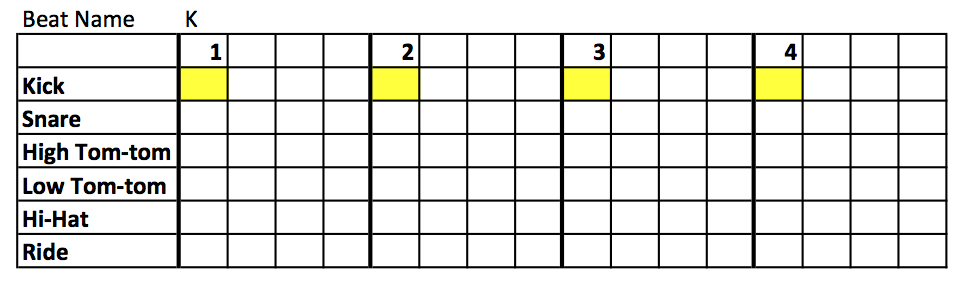
\includegraphics[scale=0.3]{images/K.jpg}\\
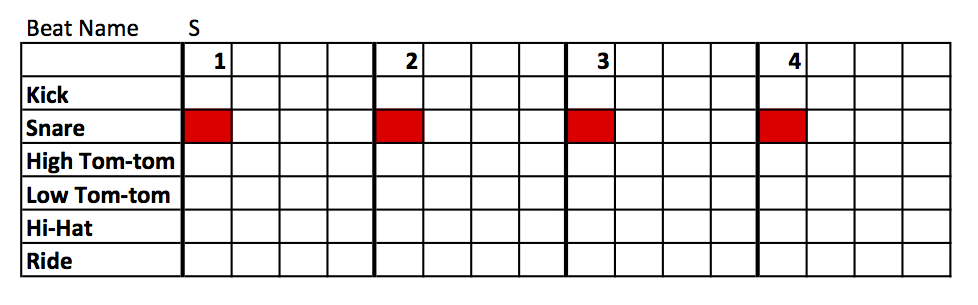
\includegraphics[scale=0.3]{images/S.jpg}\\
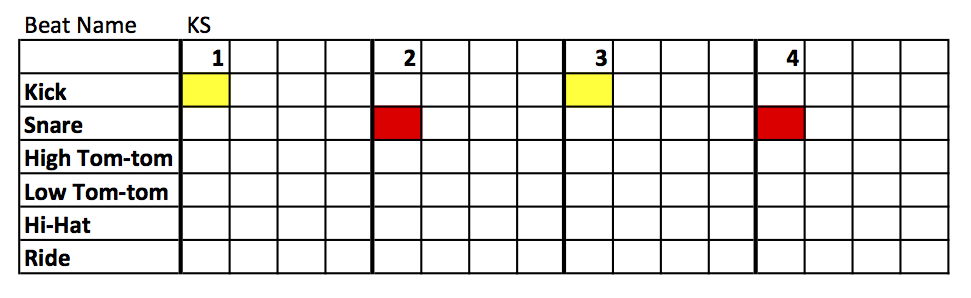
\includegraphics[scale=0.3]{images/KS.jpg}\\
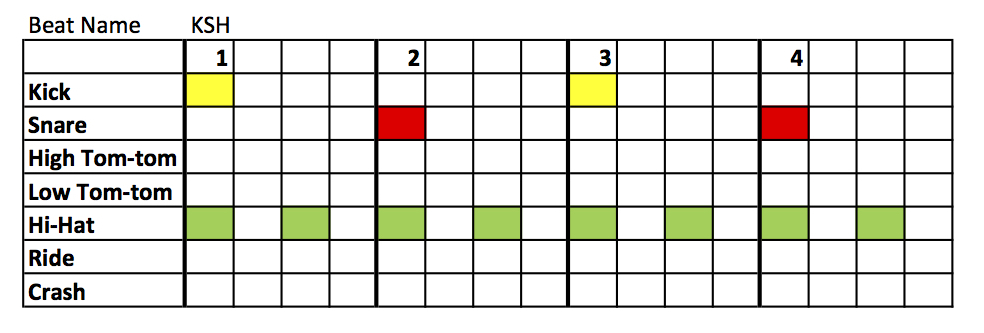
\includegraphics[scale=0.3]{images/KSH.jpg}\\
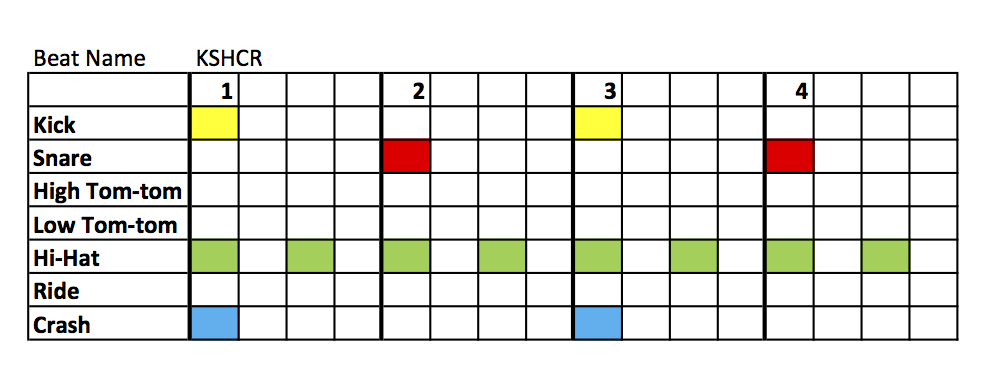
\includegraphics[scale=0.3]{images/KSHCR.jpg}\\
\includegraphics[scale=0.3]{images/HT.jpg}\\
\includegraphics[scale=0.3]{images/LT.jpg}\\
\includegraphics[scale=0.3]{images/HTLT.jpg}\\
\includegraphics[scale=0.3]{images/KSHHTLT.jpg}\\
\includegraphics[scale=0.25]{images/KS2.jpg}\\
\includegraphics[scale=0.25]{images/KSH2.jpg}\\
\includegraphics[scale=0.25]{images/KSH2CR.jpg}\\
\includegraphics[scale=0.3]{images/OFF-KSH.jpg}\\
\includegraphics[scale=0.3]{images/OFF-KSHFTTF.jpg}\\
\includegraphics[scale=0.3]{images/OFF-KSHCRFTTF.jpg}\\
\includegraphics[scale=0.25]{images/SW-K.jpg}\\
\includegraphics[scale=0.25]{images/SW-H.jpg}\\
\includegraphics[scale=0.25]{images/SW-R.jpg}\\
\includegraphics[scale=0.25]{images/SW-KH.jpg}\\
\includegraphics[scale=0.25]{images/SW-SH.jpg}\\
\includegraphics[scale=0.25]{images/SW-KSH.jpg}\\




\end{document}



